% Chapter 3

\chapter{A Convex Formulation for Multi-Task Learning} % Write in your own chapter title
\label{Chapter4}
\lhead{Chapter \ref{Chapter4}. 
\emph{A Convex Formulation for Multi-Task Learning}} % Write in your own chapter title to set the page header

{\bf \small{

}}

\section{Introduction}
% Multi-Task Learning paradigms can be divided in: Feature-Based, Parameter-Based, Joint-Learning
As we have seen in Chapter~\ref{Chapter3}, the \acrfull{mtl} proposals can be categorized as feature-based, parameter-based and combination-based approaches. Feature-based proposals have the strategy of finding a shared representation of the original features that is benefitial for all tasks. Parameter-based strategies typically use multi-task regularization schemes that, using specific regularizers, push together the parameters of the task-specialized models.
Finally, the combination-based strategies combine a common model and a task-specific one. 
%
In this chapter we will present a convex formulation for combination-based \acrshort{mtl}. With this formulation, a general task-specialized model is defined as
\begin{equation}
    \label{eq:convexmtl_general}
    \begin{aligned}
        h_r(\cdot)
       = \lambda_r g(\cdot) + (1 - \lambda_r) g_r(\cdot) .
    \end{aligned}    
\end{equation}
Here, we use the hyperparameters $\lambda_r \in [0, 1]$ to combine in a convex way the common part $g(\cdot)$ and specific parts $g_r(\cdot)$. This general formulation is very flexible, because we can use any family of functions to model $g(\cdot)$ or $g_r(\cdot)$. It is also easily interpretable, since $\lambda_r=1$ for all $r=1, \ldots, \ntasks$ results in a \acrfull{ctl} approach, while $\lambda_r=0$ leads to an \acrfull{itl} one. All the values $\lambda_r \in (0, 1)$ correspond to pure \acrshort{mtl} models, being closer to common model when $\lambda_r$ is close to $1$ and more specific when $\lambda_r$ is close to $0$.
%
Given an \acrshort{mtl} sample 
$$\bsample = \bigcup_{r=1}^\ntasks \{(x_1^r, y_1^r), \ldots, (x_{\npertask_r}^r, y_{\npertask_r}^r)\},$$
the \acrshort{mtl} regularized risk functional that corresponds to this convex formulation is 
\begin{equation}
    \label{eq:convexmtl_general_regrisk}
    \risk_{\bsample} ({g, g_1, \ldots, g_\ntasks}) = C\sum_{r=1}^{\ntasks} \sum_{i=1}^{\npertask_r} \lossf(\lambda_r g(x_i^r) + (1 - \lambda_r) g_r(x_i^r), y_i^r) + \Omega(g) + \sum_{r=1}^\ntasks \Omega_r(g_r) ,
\end{equation}
where $\Omega(g)$ and $\Omega_r(g_r)$ are the regularizers for the common and $r$-th task parts, respectively. Observe that, since the regularization is made independently for each part, no multi-task specific regularization scheme is needed. The task coupling is made directly in the definition of the model, which combines common and specific parts, and the risk $\risk_{\bsample}$ is optimized jointly in all parts.
This has some advantages, for example, no additional regularizations for coupling are needed, which usually are not convex, and there is no need to develop a new optimization procedure. In this chapter these characteristics will be presented in specific models using this convex \acrshort{mtl} formulation. We will propose convex \acrshort{mtl} formulations for kernel methods, such as the L1, L2 or LS-\acrfull{svm}, and also for \acrfull{nns}.
%

Moreover, we also present a natural alternative to convex \acrshort{mtl}, which is to combine independently trained models. That is, given a common model $g^*(\cdot)$ trained with data from all tasks, and task-specific models $g_r(\cdot)$ trained with only the data corresponding to their task, we can minimize 
\begin{equation}
    \label{eq:convexmtl_combination}
    \risk_{\bsample} (\lambda) = C\sum_{r=1}^{\ntasks} \sum_{i=1}^{\npertask_r} \lossf(\lambda_r g^*(x_i^r) + (1 - \lambda_r) g^*_r(x_i^r), y_i^r)  .
\end{equation}
Here, the models $g^*$ and $g^*_1, \ldots, g^*_\ntasks$ are fixed, and the goal is to select the optimal parameters $\lambda^*_r$ that minimize the training risk.

%
More specifically, in Section~\ref{sec:convexmlt_kernel} we present the convex \acrshort{mtl} formulation for kernel methods, and in Section~\ref{sec:convexmlt_network} we do it for \acrshort{nns}.
Finally, in Section~\ref{sec:optimal_comb} we present the alternative method of combining pre-trained models in a convex manner, proposing methods to select the optimal combination parameter for different loss functions.
%




%\section{Convex Multi-Task Learning with Kernel Methods}
\section{Convex Multi-Task Learning with Kernel Methods}
\label{sec:convexmlt_kernel}


% Kernel Methods are powerful: Kernel trick, high dimensionality representation
As explained in the previous chapters, kernel methods offer many good properties such as an implicit transformation to a possibly infinite-dimensional space and the convexity of the problems that have to be solved for the training process. With these models, such as the L1, L2 or LS-\acrshort{svm}, a regularized risk problem like the following one is solved,
% General formulation for a kernel model
%A general formulation of a training problem for kernel methods is 
\begin{equation}
    \label{eq:regrisk_kernel}
    \emprisk({w}) = \sum_{i=1}^{\nsamples} \lossf(\dotp{w}{\phi({x}_i)} + b, y_i) + \mu \Omega({w}) ,
\end{equation}
where $\sample$ is the sample $\{(x_1, y_1), \ldots, (x_\nsamples, y_\nsamples)\}$ and $\Omega(w)$ is a regularizer for ${w}$, typically the $L_2$ norm: $\norm{w}^2$. Observe that $b$, the bias term, is not regularized since it does not affect the capacity of the hypothesis space.
In~\eqref{eq:regrisk_kernel} $\phi$ is a fixed transformation function such that there exists a ``kernel trick'', that is a kernel function $k$ for which
\begin{equation}
    \nonumber
    \dotp{\phi(x)}{\phi(y)} = k(x, y).
\end{equation}
Here, $\phi$ is an element of an \acrshort{rkhs}, where $k$ is the reproducing kernel. 
The Representer Theorem~\citep*{ScholkopfHS01} states that the optimal solution of problem~\eqref{eq:regrisk_kernel} has the following form
\begin{equation}
    \nonumber
    w^* = \sum_{i=1}^\nsamples \alpha_i \phi(x_i) ,
\end{equation}
where $\alpha_i \in \reals$ are some coefficients. This means that our optimal solution $w^*$ is also an element of the same \acrshort{rkhs}.
These models embrace the Structural Risk Minimization paradigm by limiting the capacity of the space of hypothesis, which is done by penalizing the $L_2$ norm of $w$. This is equivalent to limiting our space of candidates to vectors inside a ball of some fixed radius.

% One of the first multi-task learning approach with kernel methods is Regularized \acrshort{mtl}
Multi-Task Learning with kernel methods require imposing some kind of coupling between the models for each task in the learning process. The feature learning or feature sharing approach, which is usually adopted with neural networks, is not feasible when using kernel methods, since the (implicit) transformation functions $\phi$ used are not learned but fixed, and determined by the choice of the kernel function. Therefore, other strategies have to be developed. 
One of the first approaches to \acrshort{mtl} with kernel methods was developed in~\cite{EvgeniouP04}, and later extended in~\citet{CaiC09, CaiC12}, where they use an L1-SVM formulation and the model for each task are defined as
\begin{equation}
    \nonumber
    {w}_r = {w} + {v}_r,
\end{equation} 
where $w$ is a common part, shared by all models, and $v_r$ is a task-specific part. With this approximation, the transfer of information is performed by the common part ${w}$.
The regularized risk that is minimized is then
\begin{equation}
    \label{eq:additive_regrisk}
    \risk_{\bsample} ({w, v_1, \ldots, v_\ntasks}) = C \sum_{r=1}^{\ntasks} \sum_{i=1}^{\npertask_r} \lossf(
        \dotp{w}{\phi({x}_i^r)} + \dotp{{v}_r^\intercal}{\phi_r({x}_i^r)} + b_r, y_i^r) + \mu \norm{{w}}^2 + \sum_{r=1}^\ntasks \norm{{v}_r}^2,
\end{equation}
where $\mu_c$ and $\mu_s$ are the hyperparameters to control the regularization of the common and specific parts, respectively. 
%Here $\bsample$ is an \acrshort{mtl} sample defined as $$\bsample = \bigcup_{r=1}^\ntasks \{(x_1^r, y_1^r), \ldots, (x_{\npertask_r}^r, y_{\npertask_r}^r)\}.$$
Observe also that in~\eqref{eq:additive_regrisk} different transformations are used: the transformation $\phi$ corresponds to the common part of the model, while $\phi_r$ is task-specific.
%
This is a joint learning approach that is developed for the L1-\acrshort{svm}, to which the authors give the name of \emph{Regularized \acrshort{mtl}}, but we will refer to it as the {additive} \acrshort{mtl} approach.
The influence of the hyperparameters $C$ and $\mu$ is not straightforward, and the behaviour of the solutions is asymptotical. For example, when $\mu \to \infty$, the common part $w$ disappears, and we end up with independent models for each task. Also, with $C$ and $\mu$ large enough, the result is the contrary, getting a common model for all tasks.
% %
% Observe that as $\frac{\mu_c}{\mu_s} \tendsto{}{\infty} $, we would have a common part ${w}$ that tends to zero, which would result in independent models for each task, i.e. ${w}_r \approx {v}_r$. On the contrary, when $\frac{\mu_c}{\mu_s} \tendsto{}{0} $, the task-specific parts tend to zero and every model is the common part, i.e. ${w}_r \approx {w}$.
% There are two asymptotical behaviours: the first one tends to an \acrfull{itl} approach, while the second one tends to a \acrfull{ctl} one. The \acrshort{mtl} formulation is a strategy that lies between those two approaches, \acrshort{ctl} and \acrshort{itl}, combining them to achieve a more flexible model.

% % General formulation for a convex \acrshort{mtl} Kernel 
% The asymptotical properties of this approach offer an interpretation to understand the influence of each hyperparameter, but they are not easily applicable in practice.
% We propose an alternative formulation for this joint learning approach in~\cite{RuizAD19}. The models for each task are defined as a convex combination of the common and task specific parts:
% \begin{equation}
%     \nonumber
%     {w}_r = \lambda {w} + (1 - \lambda) {v}_r,
% \end{equation}
% where $\lambda \in \left[0, 1\right]$ is a hyperparameter.
To obtain a more interpretable formulation, here we propose to use our convex \acrshort{mtl} framework of~\eqref{eq:convexmtl_general} and define the common part as $g(\cdot) =  {w}^\intercal {\phi(\cdot)} + b$ and the task-specific parts as $g_r(\cdot) = {v_r}^\intercal {\phi_r(\cdot)} + b_r$, so the \acrshort{mtl} models are
\begin{equation}
    \label{eq:convexmtl_modeldef}
    h_r(\cdot) = \lambda_r \left\lbrace {w}^\intercal {\phi(\cdot)} + b \right\rbrace + (1 - \lambda_r) \left\lbrace {v}_r^\intercal {\phi_r(\cdot)} + d_r \right\rbrace ,
\end{equation}
where $\lambda_r \in \left[0, 1\right]$ is a hyperparameter and the corresponding regularized risk is 
\begin{equation}
    \nonumber
    \begin{aligned}
        \risk_{\bsample} ({w, v_1, \ldots, v_\ntasks}) = &\sum_{r=1}^{\ntasks} \sum_{i=1}^{\npertask_r} \lossf(\lambda_r \left\lbrace {w}^\intercal {\phi(x_i^r)} + b \right\rbrace + (1 - \lambda_r) \left\lbrace {v}_r^\intercal {\phi_r(x_i^r)} + d_r \right\rbrace, y_i^r) \\ 
        &\qquad + \norm{{w}}^2 + \sum_{r=1}^\ntasks \norm{{v}_r}^2 .
    \end{aligned}
\end{equation}
We will name this approach {convex}, in contrast to the {additive} approach of the original formulation.
% Discussion?
Here, the interpretation of simpler. The model with $\lambda_r = 1$ for $r=1, \ldots, \ntasks$ is equivalent to learning a single common model for all tasks, that is ${w}_r = {w}$, while with $\lambda_r=0$, the models for each task are completely independent, i.e. ${w}_r = {v}_r$.
% The convex formulation also defines an \acrshort{mtl} model that is between a \acrshort{ctl} approach and an \acrshort{itl} one, but it presents an advantage over the additive one: the values of $\lambda$ that recover the \acrshort{ctl} and \acrshort{itl} approaches are known, and these values are attainable, that is, it is not an asymptotical behaviour as in the additive formulation. 
%

Moreover, we show that the two formulations, the {additive} and {convex}, are equivalent within an L1-\acrshort{svm} setting.
%
Finally, we also present extensions for L2 and LS-\acrshort{svm} setting in~\cite{RuizAD21}, where we apply the convex \acrshort{mtl} formulation.

%\subsection{L1-SVM and Equivalence Results}\label{subsec:cvx_l1-svm}
% The \acrfull{svm}, or L1-\acrshort{svm},~\citep{Vapnik00} is one of the most successful methods in \acrfull{ml}, since it provides a robust framework that offer good generalization properties. It is also the basis of the \acrshort{mtl} formulation in~\cite{EvgeniouP04}, where they present what we call the additive \acrshort{mtl} \acrshort{svm}, or, simply, the additive approach.
% We will present the development for the {additive} approach and for the {convex} one using an L1-\acrshort{svm} setting. Then, we will show the equivalence between the two approaches and discuss their differences.

\subsection{Additive Multi-Task Learning SVM}
%\paragraph*{{Additive} \acrshort{mtl} L1-\acrshort{svm}\\}
% Additive Approach
%   Primal
The {additive} \acrshort{mtl} primal problem formulation, presented in~\cite{EvgeniouP04} 
and extended for multiple kernel functions and task-specific biases in~\cite{CaiC12}, is the following one,
\begin{equation}\label{eq:svmmtl_primal_add}
    \begin{aligned}
    & \argmin_{w, \fv{v}, b, \fv{d}, \xi}
    & & {J({w}, \fv{v}, b, \fv{d}, \fv{\xi}) = C \sum_{r= 1}^T \sum_{i=1}^{m_r} {\xi_{i}^r} + \frac{1}{2} \sum_{r= 1}^T{\norm{{v}_r}^2} + \frac{\mu}{2} {\norm{{w}}}^2} \\
    & \text{s.t.}
    & & y_{i}^r (\dotp{w}{\phi(x_{i}^r)} + \dotp{v_r}{\phi_r(x_{i}^r)} + b_r) \geq p_{i}^r - \xi_{i}^r ,  \\
    & & & \xi_{i}^r \geq 0; \;  i=1 , \dotsc , m_r, \;  r= 1,\dotsc, T  . \\
    \end{aligned}
\end{equation}
Here, we are using the unified formulation of~\comm{TODO: Explicar formulación unificada.\\}
The prediction model is then 
\begin{equation}
    \nonumber
    h_r(\cdot) = \dotp{w}{\phi(\cdot)} + \dotp{{v}_r}{\phi_r(\cdot)} + b_r
\end{equation}
for regression and 
\begin{equation}
    \nonumber
    h_r(\cdot) = \sign{ \left(\dotp{w}{\phi(\cdot)} + \dotp{{v}_r}{\phi_r(\cdot)} + b_r \right)}
\end{equation}
for classification.
Observe again that the transformation $\phi$ is used for the common part, while the transformation $\phi_r$ is task-specific.

%
In~\eqref{eq:svmmtl_primal_add} there are two kind of hyperparameters: $C$ and $\mu$, which, in combination, balance the different parts of the objective function. 
%
Hyperparameter $C$ plays the same role than in the standard L1-\acrshort{svm}: it balances the tradeoff between the loss incurred by the model, represented by the slack variables $\xi_i^r$ and the complexity of the models, represented by the norms $\norm{{w}}$ and $\norm{{v}_r}$. Large values of $C$ highly penalize the loss, so the resulting models are more complex because they have to adapt to the training sample distribution, but these models tend to overfit. Small values of $C$ penalize more the norms of $w$ and $v_r$, hence the resulting models are simpler but not so dependent on the training sample.

%
The hyperparameter $\mu$, in combination with $C$, balances how common or specific the models are. 
Large values of $\mu$, penalize the common part, resulting in more specific models; while small values of $\mu$, alongside large values of $C$, result in a vanishing regularization of the specific parts which leads to common models.
We can distinguish the following cases:
\begin{itemize}
    \item Reduction to an \acrshort{itl} approach:
    $$\mu \tendsto{}{\infty} \implies h_r(\cdot) = \dotp{{v}_r}{\phi_r(\cdot)} + b_r .$$
    That is, the models are learned independently because the common part vanishes.
    \item Reduction to a \acrshort{ctl} approach (with task-specific biases): 
    $$C \tendsto{}{0}, \mu \tendsto{}{0} \implies h_r(\cdot) = \dotp{w}{\phi(\cdot)} + b_r .$$
    That is, the model is common for all tasks because the specific parts disappear.
    \item Pure \acrshort{mtl} approach:
    %$$ \mu_\text{inf} < \mu < \mu_\text{sup} \implies h_r(\cdot) =(\dotp{w}{\phi(\cdot)} ) + (\dotp{{v}_r}{\phi_r(\cdot)}) + b_r .$$
    $$ 0 < \mu < \infty \implies h_r(\cdot) =(\dotp{w}{\phi(\cdot)} ) + (\dotp{{v}_r}{\phi_r(\cdot)}) + b_r .$$
    There is a range of $\mu$, which depends on each specific problem, in which the models combine a common and task-specific parts.
\end{itemize}
%   Lagrangian/KKT

Observe that~\eqref{eq:svmmtl_primal_add} is a convex problem. As in the standard case of the L1-\acrshort{svm}, the corresponding dual problem is solved. To obtain the dual problem, it is necessary to express the Lagrangian of problem~\eqref{eq:svmmtl_primal_add},
\begin{equation}\label{eq:svmmtl_lagrangian_add}
    \begin{aligned}
        & \lagr({w}, \fv{v}, \fv{b}, \fv{\xi}, \fv{\alpha}, \fv{\beta}) \\
        &= C \sum_{r= 1}^T \sum_{i=1}^{m_r} {\xi_{i}^r} + \frac{1}{2} \sum_{r= 1}^T{\norm{{v}_r}^2} + \frac{\mu}{2} {\norm{{w}}}^2 \\
        &\quad -  \sum_{r= 1}^T \sum_{i=1}^{m_r} \alpha_i^r \left\lbrace y_{i}^r \left[ \dotp{w}{\phi(x_{i}^r)} + \dotp{{v}_r}{\phi_r(x_{i}^r)} + b_r \right] - p_{i}^r + \xi_{i}^r  \right\rbrace \\
        &\quad -  \sum_{r= 1}^T \sum_{i=1}^{m_r} \beta_i^r \xi_i^r ,
    \end{aligned}
\end{equation}
where $\alpha_i^r, \beta_i^r \geq 0$ are the Lagrange multipliers. Here $\fv{\xi}$ represents the vector $$(\xi_1^1, \ldots, \xi_{m_1}^1, \ldots, \xi_1^\ntasks, \ldots, \xi_{m_\ntasks}^\ntasks)^\intercal$$ and we define $\fv{\alpha}$ and $\fv{\beta}$ analogously. For compactness we also use
$$ \fv{v} = (v_1^\intercal, \ldots, v_\ntasks^\intercal)^\intercal,\; \fv{b} = (b_1, \ldots, b_\ntasks).$$
Recall that the dual objective function is defined as 
\begin{equation}\nonumber
    \begin{aligned}
         \Theta(\fv{\alpha}, \fv{\beta}) &=  \min_{{w}, \fv{v}, b, b_1, \ldots, b_\ntasks, \fv{\xi}} \lagr({w}, \fv{v}, \fv{b}, \fv{\xi}, \fv{\alpha}) \\
         &= \lagr(\optim{{w}}, \optim{\fv{v}}, \optim{\fv{b}}, \optim{\fv{\xi}}, \fv{\alpha}, \fv{\beta})
    \end{aligned}    
\end{equation}
Since $\lagr$ is convex with respect to the primal variables, it is just necessary to compute the corresponding gradients
\begin{align}
    \grad_{{w}} \lagr  = 0  &\implies \mu \optim{{w}} - \sum_{r= 1}^T \sum_{i=1}^{m_r} {\alpha_i^r} \left\lbrace y_i^r \phi(x_i^r) \right\rbrace = 0 , \label{eq:common_repr_add} \\
    \grad_{{v}_r} \lagr  = 0 &\implies \optim{{v}_r} - \sum_{i=1}^{m_r} {\alpha_i^r} \left\lbrace y_i^r \phi_r(x_i^r) \right\rbrace = 0 , \label{eq:specific_repr_add} \\
    % \grad_{b} \lagr  = 0  &\implies \sum_{r= 1}^T \sum_{i=1}^{m_r} {\alpha_i^r} y_i^r = 0 , \label{eq:common_eqconstr_add}  \\
    \grad_{b_r} \lagr  = 0 &\implies \sum_{i=1}^{m_r} {\alpha_i^r} y_i^r = 0 , \label{eq:specific_eqconstr_add} \\
    \grad_{\xi_i^r} \lagr  = 0 &\implies C - {\alpha_i^r} - {\beta_i^r} = 0 .\label{eq:xi_feas_add}
\end{align}
% \begin{align}
%     \grad_{{w}} \lagr \vert_{\optim{{w}}, \optim{\fv{v}}, \optim{b}, \optim{d_1}, \ldots, \optim{b_\ntasks}, \optim{\fv{\xi}}, \optim{\fv{\alpha}}, \optim{\fv{\beta}}} = 0  &\implies \mu \optim{{w}} - \sum_{r= 1}^T \sum_{i=1}^{m_r} \optim{\alpha_i^r} \left\lbrace y_i^r \phi(x_i^r) \right\rbrace = 0 \\
%     \grad_{{v}_r} \lagr \vert_{\optim{{w}}, \optim{\fv{v}}, \optim{b}, \optim{d_1}, \ldots, \optim{b_\ntasks}, \optim{\fv{\xi}}, \optim{\fv{\alpha}}, \optim{\fv{\beta}}} = 0 &\implies \optim{{v}_r} - \sum_{i=1}^{m_r} \optim{\alpha_i^r} \left\lbrace y_i^r \phi_r(x_i^r) \right\rbrace = 0 \\
%     \grad_{b} \lagr \vert_{\optim{{w}}, \optim{\fv{v}}, \optim{b}, \optim{d_1}, \ldots, \optim{b_\ntasks}, \optim{\fv{\xi}}, \optim{\fv{\alpha}}, \optim{\fv{\beta}}} = 0  &\implies \sum_{r= 1}^T \sum_{i=1}^{m_r} \optim{\alpha_i^r} y_i^r = 0  \\
%     \grad_{{v}_r} \lagr \vert_{\optim{{w}}, \optim{\fv{v}}, \optim{b}, \optim{d_1}, \ldots, \optim{b_\ntasks}, \optim{\fv{\xi}}, \optim{\fv{\alpha}}, \optim{\fv{\beta}}} = 0 &\implies \sum_{r= 1}^T \sum_{i=1}^{m_r} \optim{\alpha_i^r} y_i^r = 0 \\
%     \grad_{\xi_i^r} \lagr \vert_{\optim{{w}}, \optim{\fv{v}}, \optim{b}, \optim{d_1}, \ldots, \optim{b_\ntasks}, \optim{\fv{\xi}}, \optim{\fv{\alpha}}, \optim{\fv{\beta}}} = 0 &\implies C - \optim{\alpha_i^r} - \optim{\beta_i^r} = 0
% \end{align}

Using these results and substituting back in the Lagrangian we obtain
\begin{equation}\nonumber
    \begin{aligned}
        &  \lagr(\optim{{w}}, \optim{\fv{v}}, \optim{b_1}, \ldots, \optim{b_\ntasks}, \optim{\fv{\xi}}, \fv{\alpha}, \fv{\beta}) =\\
        &\quad =  \frac{1}{2} \sum_{r= 1}^T{\norm{\sum_{i=1}^{m_r} {\alpha_i^r} \left\lbrace y_i^r \phi_r({x}_i^r) \right\rbrace}^2} + \frac{\mu}{2} {\norm{ \frac{1}{\mu}\sum_{r= 1}^T \sum_{i=1}^{m_r} {\alpha_i^r} \left\lbrace y_i^r \phi({x}_i^r) \right\rbrace}}^2 \\
        &\qquad -  \sum_{r= 1}^T \sum_{i=1}^{m_r} \alpha_i^r \left\lbrace y_{i}^r \left[ \left(\frac{1}{\mu} \sum_{s= 1}^T \sum_{j=1}^{m_s} {\alpha_j^s} \left\lbrace y_j^s \phi({x}_j^s) \right\rbrace \right) \cdot \phi({x}_{i}^r) \right]  \right\rbrace \\
        &\qquad -  \sum_{r= 1}^T \sum_{i=1}^{m_r} \alpha_i^r \left\lbrace y_{i}^r \left[  \left( \sum_{j=1}^{m_r} {\alpha_j^r} \left\lbrace y_j^r \phi_r({x}_j^r) \right\rbrace \right) \cdot \phi_r({x}_{i}^r)  \right]  \right\rbrace \\
        &\qquad -  \sum_{r= 1}^T \sum_{i=1}^{m_r} \alpha_i^r \left\lbrace - p_{i}^r  \right\rbrace \\
        &\quad =  \frac{1}{2} \sum_{r= 1}^T{\dotp{\sum_{i=1}^{m_r} {\alpha_i^r} \left\lbrace y_i^r \phi_r({x}_i^r) \right\rbrace}{\sum_{i=1}^{m_r} {\alpha_i^r} \left\lbrace y_i^r \phi_r({x}_i^r) \right\rbrace}} \\
        &\qquad + \frac{\mu}{2} {\dotp{ \frac{1}{\mu}\sum_{r= 1}^T \sum_{i=1}^{m_r} {\alpha_i^r} \left\lbrace y_i^r \phi({x}_i^r) \right\rbrace}{ \frac{1}{\mu}\sum_{r= 1}^T \sum_{i=1}^{m_r} {\alpha_i^r} \left\lbrace y_i^r \phi({x}_i^r) \right\rbrace}} \\
        &\qquad - \frac{1}{\mu} \dotp{ \sum_{r= 1}^T \sum_{i=1}^{m_r} {\alpha_i^r} \left\lbrace y_i^r \phi({x}_i^r) \right\rbrace}{ \sum_{r= 1}^T \sum_{i=1}^{m_r} {\alpha_i^r} \left\lbrace y_i^r \phi({x}_i^r) \right\rbrace} \\
        &\qquad -  \sum_{r= 1}^T {\dotp{\sum_{i=1}^{m_r} {\alpha_i^r} \left\lbrace y_i^r \phi_r({x}_i^r) \right\rbrace}{\sum_{i=1}^{m_r} {\alpha_i^r} \left\lbrace y_i^r \phi_r({x}_i^r) \right\rbrace}} \\
        &\qquad -  \sum_{r= 1}^T \sum_{i=1}^{m_r} \alpha_i^r \left\lbrace - p_{i}^r  \right\rbrace \\
        &\quad = - \frac{1}{2\mu} \dotp{ \sum_{r= 1}^T \sum_{i=1}^{m_r} {\alpha_i^r} \left\lbrace y_i^r \phi({x}_i^r) \right\rbrace}{ \sum_{r= 1}^T \sum_{i=1}^{m_r} {\alpha_i^r} \left\lbrace y_i^r \phi({x}_i^r) \right\rbrace} \\
        &\qquad - \frac{1}{2} \sum_{r= 1}^T {\dotp{\sum_{i=1}^{m_r} {\alpha_i^r} \left\lbrace y_i^r \phi_r({x}_i^r) \right\rbrace}{\sum_{i=1}^{m_r} {\alpha_i^r} \left\lbrace y_i^r \phi_r({x}_i^r) \right\rbrace}} \\
        &\qquad +  \sum_{r= 1}^T \sum_{i=1}^{m_r} \alpha_i^r  p_{i}^r .
    \end{aligned}
\end{equation}
Observe that $\fv{\beta}$ has disappeared from the Lagrangian.
%   Dual
Then, the dual problem can be defined as $\min_{\fv{\alpha}} \Theta(\fv{\alpha})$ where 
$$ \Theta(\fv{\alpha}) = - \lagr(\optim{{w}}, \optim{\fv{v}}, \optim{b}, \optim{\fv{d}}, \optim{\fv{\xi}}, \fv{\alpha}, \fv{\beta}), $$
and $\fv{\alpha}$ must fulfill the KKT conditions, that is~\comm{TODO: Explicar KKT }. 
The condition~\eqref{eq:xi_feas_add}, using that $\alpha_i^r , \beta_i^r \geq 0$, implies $0 \leq \alpha_i^r \leq C$. Taking into account these KKT conditions, the dual problem can be expressed as
\begin{equation}\label{eq:svmmtl_dual_add}
    \begin{aligned}
    & \min_{\alpha} & \Theta(\alpha) &=  \frac{1}{2\mu} \dotp{ \sum_{r= 1}^T \sum_{i=1}^{m_r} {\alpha_i^r} \left\lbrace y_i^r \phi({x}_i^r) \right\rbrace}{ \sum_{r= 1}^T \sum_{i=1}^{m_r} {\alpha_i^r} \left\lbrace y_i^r \phi({x}_i^r) \right\rbrace} \\
    & & &\quad + \frac{1}{2} \sum_{r= 1}^T {\dotp{\sum_{i=1}^{m_r} {\alpha_i^r} \left\lbrace y_i^r \phi_r({x}_i^r) \right\rbrace}{\sum_{i=1}^{m_r} {\alpha_i^r} \left\lbrace y_i^r \phi_r({x}_i^r) \right\rbrace}}  - \sum_{r=1}^\ntasks \sum_{i=1}^{\npertask_r} \alpha_i^r p_i^r ,\\
    & \text{s.t.}
    & & 0 \leq \alpha_i^r \leq C ; \; i=1, \ldots, \npertask_r;\;\; r=1, \ldots, \ntasks \\
    & & & \sum_{i=1}^{m_r} \alpha_i^r y_i^r = 0;\;  r=1, \ldots, \ntasks , \\
    \end{aligned}
\end{equation}
where there are  task-specific equality constraints that have its origin in Equation~\eqref{eq:specific_eqconstr_add}.
Using the kernel trick, we can write the dual problem with a matrix formulation
\begin{equation}\label{eq:svmmtl_dualvec_add}
    \begin{aligned}
    & \min_{\alpha} && \Theta(\alpha) = \frac{1}{2} \fv{\alpha}^\intercal \left(\frac{1}{\mu} \fm{Q} + \fm{K} \right) \fv{\alpha} - \fv{p} \fv{\alpha} \\
    & \text{s.t.}
    & & 0 \leq \alpha_i^r \leq C ; \; i=1, \ldots, \npertask_r;\;\; r=1, \ldots, \ntasks ,\\
    & & & \sum_{i=1}^{m_r} \alpha_i^r y_i^r = 0;\;  r=1, \ldots, \ntasks . \\
    \end{aligned}
\end{equation}
Here $Q$ and $K$ are the common and specific kernel matrices, respectively.
The matrix $Q$ is generated using the common kernel, defined as 
\begin{equation}
    \nonumber
    k(x_i^r, x_j^s) = \dotp{\phi(x_i^r)}{\phi(x_j^s)} .
\end{equation}
and $K$ is the block-diagonal matrix built using the kernel
\begin{equation}
    \nonumber
    k_r(x_i^r, x_j^s) = \delta_{rs} \dotp{\phi_r(x_i^r)}{\phi_s(x_j^s)} ,
\end{equation}
that is,
\begin{equation}
    \nonumber
    \fm{Q} = 
    \begin{pmatrix}
    \underbrace{Q_{1, 1}}_{m_1 \times m_1} & \underbrace{\fm{Q}_{1, 2}}_{m_1 \times m_2} & \underbrace{\fm{Q}_{1, 3}}_{m_1 \times m_3} & \cdots & \underbrace{\fm{Q}_{1, T}}_{m_1 \times m_T} \\
    \underbrace{\fm{Q}_{2, 1}}_{m_2 \times m_1} & \underbrace{Q_{2, 2}}_{m_2 \times m_2} & \underbrace{\fm{Q}_{2, 1}}_{m_2 \times m_1} & \cdots & \underbrace{\fm{Q}_{2, T}}_{m_2 \times m_T} \\
    \vdots      & \vdots &\vdots    & \ddots & \vdots \\
    \underbrace{\fm{Q}_{T, 1}}_{m_T \times m_1} & \underbrace{\fm{Q}_{T, 2}}_{m_T \times m_2} & \underbrace{\fm{Q}_{T, 3}}_{m_T \times m_3} & \cdots & \underbrace{\fm{Q}_{\ntasks, \ntasks}}_{m_\ntasks \times m_\ntasks}
    \end{pmatrix} ,
\end{equation}
where each block $\fm{Q}_{r,s}$ is defined as
\begin{equation}
    \label{eq:kernelmatrix_common}
    \fm{Q}_{r, s} = \begin{pmatrix}
    y_1^r y_1^s k({x}_1^r, {x}_1^s) & y_1^r y_2^s k({x}_1^r, {x}_2^s) & \cdots & y_1^r y_{m_s}^s k({x}_1^r, {x}_{m_s}^s) \\
    y_2^r y_1^s k({x}_2^r, {x}_1^s) & y_2^r y_2^s k({x}_2^r, {x}_2^s) & \cdots & y_2^r y_{m_s}^s k({x}_2^r, {x}_{m_s}^s) \\
    \vdots & \vdots & \ddots & \vdots \\
    y_{m_r}^r y_1^s k({x}_{m_r}^r, {x}_1^s) & y_{m_r}^r y_2^s k({x}_{m_r}^r, {x}_2^s) & \cdots & y_{m_r}^r y_{m_s}^s k({x}_{m_r}^r, {x}_{m_s}^s) \\
    \end{pmatrix} ;
\end{equation}
and 
\begin{equation}
    \nonumber
    \fm{K} = 
    \begin{pmatrix}
    \underbrace{K_{1, 1}}_{m_1 \times m_1} & \underbrace{\fm{0}}_{m_1 \times m_2} & \underbrace{\fm{0}}_{m_1 \times m_3} & \cdots & \underbrace{\fm{0}}_{m_1 \times m_T} \\
    \underbrace{\fm{0}}_{m_2 \times m_1} & \underbrace{K_{2, 2}}_{m_2 \times m_2} & \underbrace{\fm{0}}_{m_2 \times m_1} & \cdots & \underbrace{\fm{0}}_{m_2 \times m_T} \\
    \vdots      & \vdots &\vdots    & \ddots & \vdots \\
    \underbrace{\fm{0}}_{m_T \times m_1} & \underbrace{\fm{0}}_{m_T \times m_2} & \underbrace{\fm{0}}_{m_T \times m_3} & \cdots & \underbrace{K_{\ntasks, \ntasks}}_{m_\ntasks \times \ntasks}
    \end{pmatrix} ,
\end{equation}
where each task block $\fm{K}_{r, r}$ is defined as
\begin{equation}
    \label{eq:kernelmatrix_specific}
    \fm{K}_{r, r} = \begin{pmatrix}
        y_1^r y_1^r k_r({x}_1^r, {x}_1^r) & y_1^r y_2^r k_r({x}_1^r, {x}_2^r) & \cdots & y_1^r y_{m_s}^r k_r({x}_1^r, {x}_{m_r}^r) \\
        y_2^r y_1^r k_r({x}_2^r, {x}_1^r) & y_2^r y_2^r k_r({x}_2^r, {x}_2^r) & \cdots & y_2^r y_{m_s}^r k_r({x}_2^r, {x}_{m_r}^r) \\
    \vdots & \vdots & \ddots & \vdots \\
    y_{m_r}^r y_1^r k_r({x}_{m_r}^r, {x}_1^r) & y_{m_r}^r y_2^r k_r({x}_{m_r}^r, {x}_2^r) & \cdots & y_{m_r}^r y_{m_s}^r k_r({x}_{m_r}^r, {x}_{m_r}^r) \\
    \end{pmatrix} .
\end{equation}
Combined, we have a multi-task kernel matrix $\widehat{\fm{Q}} = (1/\mu) \fm{Q} + \fm{K}$, whose corresponding multi-task kernel function can be expressed as 
\begin{equation}
    \nonumber
    \widehat{k}({x}_i^r, {x}_j^s) = \frac{1}{\mu} k({x}_i^r, {x}_j^s) + \delta_{rs} k_r({x}_i^r, {x}_j^s) .
\end{equation}
Here we are using two different kernels: a common one $k(x, \tilde{x})$ and a task-specific one $k_r(x, \tilde{x})$, each being the reproducing kernels for the common and task-specific transformations, respectively. That is,
$k(x, \tilde{x}) = \dotp{\phi(x)}{\phi(\tilde{x})}$ and $k_r(x, \tilde{x}) = \dotp{\phi_r(x)}{\phi_r(\tilde{x})}$.

%   Discussion: Primal vs Dual
The dual problem~\eqref{eq:svmmtl_dualvec_add} is very similar to the standard one \comm{TODO: poner referencia al estándar} but we have two major differences: the use of the multi-task kernel matrix $\widehat{\fm{Q}}$ and the multiple equality constraints. These constraints, which appear in~\eqref{eq:specific_eqconstr_add}, are consequence of the specific biases used in the primal problem~\eqref{eq:svmmtl_primal_add}. In~\cite{CaiC12} the authors develop a Generalized SMO algorithm to account for these multiple equality constraints.

Analyzing the hyperparameters influence in the dual problem, note that $C$ is an upper bound for the dual coefficients, as in the standard case, and the hyperparameter of interest for this \acrshort{mtl} formulation, which is $\mu$, scales the common matrix $\fm{Q}$. As with the primal formulation, we can define three different cases:
\begin{itemize}
    \item Reduction to an \acrshort{itl} approach:
    $$\mu \tendsto{}{\infty} \implies  h_r(\cdot) = \sum_{i=1}^{m_r} {\alpha_i^r} y_i^r \left\lbrace k_r(x_i^r, \cdot) \right\rbrace + b_r .$$
    Thus, the matrix is block-diagonal and optimizing the dual problem is equivalent to optimizing a specific dual problem for each task.
    \item Reduction to a \acrshort{ctl} approach (with task-specific biases): 
    $$C \tendsto{}{0}, \mu \tendsto{}{0} \implies  h_r(\cdot) = \sum_{r= 1}^T \sum_{i=1}^{m_r} {\alpha_i^r} y_i^r \left\lbrace k(x_i^r, \cdot) \right\rbrace + b_r.$$
    This is the standard dual objective function for \acrshort{ctl}.
    \item Pure \acrshort{mtl} approach:
    $$ 0 < \mu < \infty \implies h_r(\cdot) = \sum_{r= 1}^T \sum_{i=1}^{m_r} {\alpha_i^r} y_i^r \left\lbrace \frac{1}{\mu} k(x_i^r, \cdot) + k_r(x_i^r, \cdot) \right\rbrace + b_r. $$
    Here the kernel matrix combines the common and specific matrices.
\end{itemize}


\subsection{Convex Multi-Task Learning SVM}

% Convex Approach
%\paragraph*{{Convex} \acrshort{mtl} L1-\acrshort{svm}.\\}
% Additive Approach
%   Primal
We propose a convex formulation for the \acrshort{mtl} L1-\acrshort{svm}, which we have presented in~\cite{RuizAD19}. This formulation offers a better interpretability because the influence of the common and task-specific parts is more clear. 
%
The primal problem is
\begin{equation}\label{eq:svmmtl_primal_convex}
    \begin{aligned}
    & \argmin_{w, \fv{v}, b, \fv{d}, \fv{\xi}}
    & & {J({w}, \fv{v}, b, \fv{d}, \fv{\xi}) = C \sum_{r= 1}^T \sum_{i=1}^{m_r} {\xi_{i}^r} + \frac{1}{2} \sum_{r= 1}^T{\norm{{v}_r}^2} + \frac{1}{2} {\norm{{w}}}^2} \\
    & \text{s.t.}
    & & y_{i}^r \left(\lambda_r \left\lbrace \dotp{w}{\phi(x_{i}^r)} + b  \right\rbrace + (1 - \lambda_r) \left\lbrace \dotp{{v}_r}{\phi_r(x_{i}^r)} + d_r \right\rbrace  \right) \geq p_{i}^r - \xi_{i}^r ,  \\
    & & & \xi_{i}^r \geq 0; \;  i=1 , \dotsc , m_r, \;  r= 1,\dotsc, T  . \\
    \end{aligned}
\end{equation}
Here, the former hyperparameter $\mu$ used in the regularization is replaced by the hyperparameters $\lambda_r$, which are used in the model definition. The prediction model is then
\begin{equation}
    \nonumber
    h_r({\cdot}) = \lambda_r \left\lbrace \dotp{w}{\phi(\cdot)} + b  \right\rbrace + (1 - \lambda_r) \left\lbrace \dotp{{v}_r}{\phi_r(\cdot)} + d_r \right\rbrace
\end{equation}
for regression and 
\begin{equation}
    \nonumber
    h_r({\cdot}) = \sign{ \left(\lambda_r \left\lbrace \dotp{w}{\phi(\cdot)} + b  \right\rbrace + (1 - \lambda_r) \left\lbrace \dotp{{v}_r}{\phi_r(\cdot)} + d_r \right\rbrace \right)}
\end{equation}
for classification.
%

With this convex formulation, the roles of hyperparameters $C$ and $\lambda_r$ are independent. Hyperparameter $C$ regulates the trade-off between the loss and the margin size of each task-specialized model $h_r$, while $\lambda_r$ indicates how specific or common these models are in the range of $[0, 1]$. With $\lambda_r=0$ we have independent models for each task and for $\lambda_r=1$ we have a common model for all tasks. 
%
In~\eqref{eq:svmmtl_primal_convex}, depending on the value of hyperparameters $C$, $\lambda_1, \ldots, \lambda_\ntasks$, we can highlight the following situations:
%
\begin{itemize}
    \item Reduction to an \acrshort{itl} approach:
    $$\lambda_r = 0 ;\; r=1, \ldots, \ntasks \implies h_r(\cdot) = \dotp{{v}_r}{\phi_r(\cdot)} + d_r .$$
    \item Reduction to a \acrshort{ctl} approach: 
    $$ \lambda_r = 1 ;\; r=1, \ldots, \ntasks \implies h_r(\cdot) = \dotp{w}{\phi(\cdot)} + b .$$
    \item Pure \acrshort{mtl} approach:
    $$ 0 < \lambda_r < 1 ;\; r=1, \ldots, \ntasks \implies h_r(\cdot) = \lambda_r (\dotp{w}{\phi(\cdot)} + b ) + (1 - \lambda_r) (\dotp{{v}_r}{\phi_r(\cdot)} + d_r) .$$
\end{itemize}
Observe that now the cases are not unbounded but have attainable values, 0 for \acrshort{itl} and 1 for \acrshort{ctl}, while all the values in the open $(0, 1)$ yield pure \acrshort{mtl} models. Also, the parameter $C$ no longer interferes with these cases and only the $\lambda_r$ calibrate the specifity of the models.
%   Lagrangian/KKT
 The Lagrangian of problem~\eqref{eq:svmmtl_primal_convex} is
\begin{equation}\label{eq:svmmtl_lagrangian_convex}
    \begin{aligned}
        & \lagr({w}, \fv{v}, b, \fv{d}, \fv{\xi}, \fv{\alpha}, \fv{\beta}) \\
        &=  C \sum_{r= 1}^T \sum_{i=1}^{m_r} {\xi_{i}^r} + \frac{1}{2} \sum_{r= 1}^T{\norm{{v}_r}^2} + \frac{1}{2} {\norm{{w}}}^2 \\
        &\quad -  \sum_{r= 1}^T \sum_{i=1}^{m_r} \alpha_i^r \left\lbrace y_{i}^r  \left(\lambda_r \left\lbrace \dotp{w}{\phi(x_{i}^r)} + b  \right\rbrace + (1 - \lambda_r) \left\lbrace \dotp{{v}_r}{\phi_r(x_{i}^r)} + d_r \right\rbrace  \right) - p_{i}^r + \xi_{i}^r  \right\rbrace \\
        &\quad -  \sum_{r= 1}^T \sum_{i=1}^{m_r} \beta_i^r \xi_i^r ,
    \end{aligned}
\end{equation}
where $\alpha_i^r, \beta_i^r \geq 0$ are the Lagrange multipliers. Again, $\fv{\xi}$ represents the vector $$(\xi_1^1, \ldots, \xi_{m_1}^1, \ldots, \xi_1^\ntasks, \ldots, \xi_{m_\ntasks}^\ntasks)^\intercal$$ and analogously for $\fv{\alpha}$ and $\fv{\beta}$.
We also use 
$$ \fv{v} = (v_1^\intercal, \ldots, v_\ntasks^\intercal)^\intercal,\; \fv{d} = (d_1, \ldots, d_\ntasks).$$
The dual objective function is defined as 
\begin{equation}\nonumber
    \begin{aligned}
         \Theta(\fv{\alpha}, \fv{\beta}) &=  \min_{{w}, \fv{v}, b, \fv{d}, \fv{\xi}} \lagr({w}, \fv{v}, b, \fv{d}, \fv{\xi}, \fv{\alpha}, \fv{\beta}) \\
         &= \lagr(\optim{{w}}, \optim{\fv{v}}, \optim{b}, \optim{\fv{d}}, \optim{\fv{\xi}}, \fv{\alpha}, \fv{\beta})
    \end{aligned}    
\end{equation}
The gradients with respect to the primal variables are
\begin{align}
    \grad_{{w}} \lagr  = 0  &\implies \optim{{w}} - \sum_{r= 1}^\ntasks \lambda_r \sum_{i=1}^{m_r} {\alpha_i^r} \left\lbrace y_i^r \phi(x_i^r) \right\rbrace = 0 , \label{eq:common_repr_conv} \\
    \grad_{{v}_r} \lagr  = 0 &\implies \optim{{v}_r} - (1 - \lambda_r) \sum_{i=1}^{m_r} {\alpha_i^r} \left\lbrace y_i^r \phi_r(x_i^r) \right\rbrace = 0 , \label{eq:specific_repr_conv} \\
    \grad_{b} \lagr  = 0  &\implies \sum_{r= 1}^T \sum_{i=1}^{m_r} {\alpha_i^r} y_i^r = 0 , \label{eq:specific_eqconstr_conv}  \\
    \grad_{{d}_r} \lagr  = 0 &\implies \sum_{i=1}^{m_r} {\alpha_i^r} y_i^r = 0 , \label{eq:common_eqconstr_conv} \\
    \grad_{\xi_i^r} \lagr  = 0 &\implies C - {\alpha_i^r} - {\beta_i^r} = 0 . \label{eq:xi_feas_conv}
\end{align}
% \begin{align}
%     \grad_{{w}} \lagr \vert_{\optim{{w}}, \optim{\fv{v}}, \optim{b}, \optim{\fv{d}}, \optim{\fv{\xi}}, \optim{\fv{\alpha}}, \optim{\fv{\beta}}} = 0  &\implies \mu \optim{{w}} - \sum_{r= 1}^T \sum_{i=1}^{m_r} \optim{\alpha_i^r} \left\lbrace y_i^r \phi(x_i^r) \right\rbrace = 0 \\
%     \grad_{{v}_r} \lagr \vert_{\optim{{w}}, \optim{\fv{v}}, \optim{b}, \optim{\fv{d}}, \optim{\fv{\xi}}, \optim{\fv{\alpha}}, \optim{\fv{\beta}}} = 0 &\implies \optim{{v}_r} - \sum_{i=1}^{m_r} \optim{\alpha_i^r} \left\lbrace y_i^r \phi_r(x_i^r) \right\rbrace = 0 \\
%     \grad_{b} \lagr \vert_{\optim{{w}}, \optim{\fv{v}}, \optim{b}, \optim{\fv{d}}, \optim{\fv{\xi}}, \optim{\fv{\alpha}}, \optim{\fv{\beta}}} = 0  &\implies \sum_{r= 1}^T \sum_{i=1}^{m_r} \optim{\alpha_i^r} y_i^r = 0  \\
%     \grad_{{v}_r} \lagr \vert_{\optim{{w}}, \optim{\fv{v}}, \optim{b}, \optim{\fv{d}}, \optim{\fv{\xi}}, \optim{\fv{\alpha}}, \optim{\fv{\beta}}} = 0 &\implies \sum_{r= 1}^T \sum_{i=1}^{m_r} \optim{\alpha_i^r} y_i^r = 0 \\
%     \grad_{\xi_i^r} \lagr \vert_{\optim{{w}}, \optim{\fv{v}}, \optim{b}, \optim{\fv{d}}, \optim{\fv{\xi}}, \optim{\fv{\alpha}}, \optim{\fv{\beta}}} = 0 &\implies C - \optim{\alpha_i^r} - \optim{\beta_i^r} = 0
% \end{align}

Using these results and substituting back in the Lagrangian we obtain
\begin{equation}\nonumber
    \begin{aligned}
        & \lagr(\optim{{w}}, \optim{\fv{v}}, \optim{b}, \optim{\fv{d}}, \optim{\fv{\xi}}, \fv{\alpha}, \fv{\beta})\\
        &\quad=  \frac{1}{2} \sum_{r= 1}^T{\norm{ (1 - \lambda_r) \sum_{i=1}^{m_r}  {\alpha_i^r} \left\lbrace y_i^r \phi_r({x}_i^r) \right\rbrace}^2} + \frac{1}{2} {\norm{\sum_{r= 1}^T \lambda_r \sum_{i=1}^{m_r} {\alpha_i^r} \left\lbrace y_i^r \phi({x}_i^r) \right\rbrace}}^2 \\
        &\qquad - \sum_{r= 1}^T \lambda_r \sum_{i=1}^{m_r} \alpha_i^r \left\lbrace y_{i}^r \left[ \left(\sum_{s= 1}^T \lambda_r \sum_{j=1}^{m_s} {\alpha_j^s} \left\lbrace y_j^s \phi({x}_j^s) \right\rbrace \right) \cdot \phi({x}_{i}^r) \right]  \right\rbrace \\
        &\qquad -  \sum_{r= 1}^T (1-\lambda_r) \sum_{i=1}^{m_r} \alpha_i^r \left\lbrace y_{i}^r \left[  \left((1-\lambda_r) \sum_{j=1}^{m_r} {\alpha_j^r} \left\lbrace y_j^r \phi_r({x}_j^r) \right\rbrace \right) \cdot \phi_r({x}_{i}^r)  \right]  \right\rbrace \\
        &\qquad -  \sum_{r= 1}^T \sum_{i=1}^{m_r} \alpha_i^r \left\lbrace - p_{i}^r  \right\rbrace \\
        &\quad=  \frac{1}{2} \sum_{r= 1}^T{\dotp{(1-\lambda_r)\sum_{i=1}^{m_r} {\alpha_i^r} \left\lbrace y_i^r \phi_r({x}_i^r) \right\rbrace}{(1-\lambda_r)\sum_{i=1}^{m_r} {\alpha_i^r} \left\lbrace y_i^r \phi_r({x}_i^r) \right\rbrace}} \\
        &\qquad + \frac{1}{2} {\dotp{\sum_{r= 1}^\ntasks \lambda_r \sum_{i=1}^{m_r} {\alpha_i^r} \left\lbrace y_i^r \phi({x}_i^r) \right\rbrace}{\sum_{r= 1}^\ntasks \lambda_r \sum_{i=1}^{m_r} {\alpha_i^r} \left\lbrace y_i^r \phi({x}_i^r) \right\rbrace}} \\
        &\qquad - \dotp{ \sum_{r= 1}^T \lambda_r \sum_{i=1}^{m_r} {\alpha_i^r} \left\lbrace y_i^r \phi({x}_i^r) \right\rbrace}{ \sum_{r= 1}^T \lambda_r \sum_{i=1}^{m_r} {\alpha_i^r} \left\lbrace y_i^r \phi({x}_i^r) \right\rbrace} \\
        &\qquad -  \sum_{r= 1}^T {\dotp{(1-\lambda_r) \sum_{i=1}^{m_r} {\alpha_i^r} \left\lbrace y_i^r \phi_r({x}_i^r) \right\rbrace}{(1-\lambda_r) \sum_{i=1}^{m_r} {\alpha_i^r} \left\lbrace y_i^r \phi_r({x}_i^r) \right\rbrace}} \\
        &\qquad -  \sum_{r= 1}^T \sum_{i=1}^{m_r} \alpha_i^r \left\lbrace - p_{i}^r  \right\rbrace \\
        &\quad= - \frac{1}{2} \dotp{ \sum_{r= 1}^T  \lambda_r \sum_{i=1}^{m_r} {\alpha_i^r} \left\lbrace y_i^r \phi({x}_i^r) \right\rbrace}{ \sum_{r= 1}^T \lambda_r \sum_{i=1}^{m_r} {\alpha_i^r} \left\lbrace y_i^r \phi({x}_i^r) \right\rbrace} \\
        &\qquad - \frac{1}{2} \sum_{r= 1}^T {(1-\lambda_r) \dotp{\sum_{i=1}^{m_r} {\alpha_i^r} \left\lbrace y_i^r \phi_r({x}_i^r) \right\rbrace}{(1-\lambda_r) \sum_{i=1}^{m_r} {\alpha_i^r} \left\lbrace y_i^r \phi_r({x}_i^r) \right\rbrace}} \\
        &\qquad +  \sum_{r= 1}^T \sum_{i=1}^{m_r} \alpha_i^r  p_{i}^r .
    \end{aligned}
\end{equation}
%   Dual
As with the additive formulation, the dual problem can then be defined as 
\begin{equation}\label{eq:svmmtl_dual_conv}
    \begin{aligned}
    & \min_{\alpha} & \Theta(\alpha) &=  \frac{1}{2} \dotp{\sum_{r= 1}^\ntasks \lambda_r \sum_{i=1}^{m_r} {\alpha_i^r} \left\lbrace y_i^r \phi({x}_i^r) \right\rbrace}{\sum_{r= 1}^\ntasks \lambda_r \sum_{i=1}^{m_r} {\alpha_i^r} \left\lbrace y_i^r \phi({x}_i^r) \right\rbrace} \\
    & & &\quad + \frac{1}{2} \sum_{r= 1}^T {\dotp{(1 - \lambda_r)\sum_{i=1}^{m_r} {\alpha_i^r} \left\lbrace y_i^r \phi_r({x}_i^r) \right\rbrace}{(1 - \lambda_r) \sum_{i=1}^{m_r} {\alpha_i^r} \left\lbrace y_i^r \phi_r({x}_i^r) \right\rbrace}} \\
    & & &\quad - \sum_{r=1}^\ntasks \sum_{i=1}^{\npertask_r} \alpha_i^r p_i^r   \\
    & \text{s.t.}
    & & 0 \leq \alpha_i^r \leq C ; \; i=1, \ldots, \npertask_r;\;\; r=1, \ldots, \ntasks , \\
    & & & \sum_{i=1}^{m_r} \alpha_i^r y_i^r = 0;\;  r=1, \ldots, \ntasks . \\
    \end{aligned}
\end{equation}
And the matrix formulation using the kernel matrices is
\begin{equation}\label{eq:svmmtl_dualvec_conv}
    \begin{aligned}
    & \min_{\alpha} && \Theta(\alpha) = \frac{1}{2} \fv{\alpha}^\intercal \left(\Lambda \fm{Q} \Lambda + \left(\fm{I}_{\nsamples} - \Lambda \right) \fm{K} \left(\fm{I}_{\nsamples} - \Lambda \right) \right) \fv{\alpha} - \fv{p} \fv{\alpha} \\
    & \text{s.t.}
    & & 0 \leq \alpha_i^r \leq C ; \; i=1, \ldots, \npertask_r;\;\; r=1, \ldots, \ntasks ,\\
    & & & \sum_{i=1}^{m_r} \alpha_i^r y_i^r = 0;\;  r=1, \ldots, \ntasks , \\
    \end{aligned}
\end{equation}
where
\begin{equation}\label{eq:lambdamatrix_def}
    \Lambda = \Diag(\overbrace{\lambda_1, \ldots, \lambda_1}^{\npertask_1}, \ldots, \overbrace{\lambda_\ntasks, \ldots, \lambda_\ntasks}^{\npertask_\ntasks})
\end{equation}
and $\fm{I}_{\nsamples}$ is the $\nsamples \times \nsamples$ identity matrix;
here $Q$ and $K$ are the common and specific kernel matrices, respectively.
Combined, we have a multi-task kernel matrix 
\begin{equation}
    \label{eq:conv_mtl_kernel_matrix}
    \widehat{\fm{Q}} = \Lambda \fm{Q} \Lambda + \left(\fm{I}_{\nsamples} - \Lambda \right) \fm{K} \left(\fm{I}_{\nsamples} - \Lambda \right),
\end{equation}
whose corresponding multi-task kernel function can be expressed as 
\begin{equation}
    \label{eq:conv_mtl_kernel_fun}
    \widehat{k}({x}_i^r, {x}_j^s) = \lambda_r \lambda_s k({x}_i^r, {x}_j^s) +  \delta_{rs} (1-\lambda_r) (1 - \lambda_s) k_r({x}_i^r, {x}_j^s) ,
\end{equation}
where again we are using the common kernel $k(x, \tilde{x}) = \dotp{\phi(x)}{\phi(\tilde{x})}$ and the task-specific kernels $k_r(x, \tilde{x}) = \dotp{\phi_r(x)}{\phi_r(\tilde{x})}$ for $r=1, \ldots, \ntasks$.
% Then, we can define the kernel matrix as 
% \begin{equation}
%     \nonumber
%     \widehat{\fm{Q}} = 
%     \begin{pmatrix}
%         y_1^1 y_1^1 \widehat{k}(x_1^1, x_1^1) & y_1^1 y_2^1 \widehat{k}(x_1^1, x_2^1)  & \ldots & y_1^1 y_{\npertask_\ntasks}^\ntasks \widehat{k}(x_1^1, x_{\npertask_\ntasks}^\ntasks) \\
%         y_2^1 y_1^1 \widehat{k}(x_2^1, x_1^1) & y_2^1 y_2^1 \widehat{k}(x_2^1, x_2^1) & \ldots & y_2^1 y_{\npertask_\ntasks}^\ntasks \widehat{k}(x_2^1, x_{\npertask_\ntasks}^\ntasks) \\
%         \vdots & \vdots & \ddots & \vdots \\
%         y_{\npertask_\ntasks}^\ntasks y_1^1 \widehat{k}(x_{\npertask_\ntasks}^\ntasks, x_{1}^1) & y_{\npertask_\ntasks}^\ntasks y_{2}^1 \widehat{k}(x_{\npertask_\ntasks}^\ntasks, x_{2}^1) & \ldots & y_{\npertask_\ntasks}^\ntasks y_{\npertask_\ntasks}^\ntasks \widehat{k}(x_{\npertask_\ntasks}^\ntasks, x_{\npertask_\ntasks}^\ntasks) \\
%     \end{pmatrix} .
% \end{equation}

%   Discussion: Primal vs Dual
This dual problem is very similar to the one shown in~\eqref{eq:svmmtl_dualvec_add} where there are also $\ntasks$ equality constraints, but the multi-task kernel matrix $\widehat{\fm{Q}}$ is defined differently, dropping the $\mu$ hyperparameter and incorporating the $\lambda_r$ ones.
Studying the influence of $\lambda_r$ hyperparameters in the dual problem we can describe the following cases:
\begin{itemize}
    \item Reduction to an \acrshort{itl} approach:
    $$\lambda_r = 0;\; r=1, \ldots, \ntasks  \implies  h_r(\hat{x}) = \sum_{r= 1}^T \sum_{i=1}^{m_r} {\alpha_i^r} y_i^r \left\lbrace k_r(x_i^r, \hat{x}) \right\rbrace  + d_r .$$
    \item Reduction to a \acrshort{ctl} approach: 
    $$\lambda_r = 1;\; r=1, \ldots, \ntasks \implies  h_r(\hat{x}) = \sum_{r= 1}^T \sum_{i=1}^{m_r} {\alpha_i^r} y_i^r \left\lbrace k(x_i^r, \hat{x})  \right\rbrace + b .$$
    \item Pure \acrshort{mtl} approach:
    \begin{align*}
        &0 < \lambda_r < 1;\; r=1, \ldots, \ntasks \implies \\
        &\quad h_r(\hat{x}) = \sum_{r= 1}^T \sum_{i=1}^{m_r} {\alpha_i^r} y_i^r \left\lbrace \lambda_r^2 k(x_i^r, \hat{x}) + (1 - \lambda_r)^2 k_r(x_i^r, \hat{x}) \right\rbrace + \lambda_r b + (1-\lambda_r)d_r.
    \end{align*}
\end{itemize}
The properties that are found in the primal formulation are also present in the dual one. All the values of $\lambda_r$ in the open interval $(0, 1)$ correspond to pure \acrshort{mtl} approaches while the extreme values $\lambda_r=1$ and $\lambda_r=0$ correspond to \acrshort{ctl} and \acrshort{itl} approaches, respectively.



\subsection{Equivalence between Convex and Additive MTL SVM}\label{subsec:equiv}

% \paragraph*{Equivalence Results.\\}
% Equivalence results
Both the {additive} and {convex} \acrshort{mtl} \acrshort{svm} approaches solve a similar problem, but there is a change in the formulation to get rid of a regularization hyperparameter $\mu$ in favor of those defining convex combination of models, hyperparameters $\lambda_r$.
Both approaches offer similar properties: allowing the value of their hyperparameters to go from completely common to completely independent models, and passing through pure multi-task models.
However, it is not obvious what is the relation between those two approaches.
% Lemmas
In~\cite{RuizAD19} we provide two propositions to show the equivalence between {additive} and {convex} \acrshort{mtl} \acrshort{svm} formulations where a common $\lambda$ is used.
\begin{prop}\label{prop:add_conv_equiv}
    The {additive} \acrshort{mtl}-\acrshort{svm} primal problem with parameters $C_\text{add}$ and $\mu$ (and possibly $\epsilon$), that is,
    \begin{equation}\label{eq:svmmtl_primal_add_equiv}
        \begin{aligned}
        & \argmin_{w, \fv{v}, b, \fv{d}, \xi}
        & & {J({w}, \fv{v}, b, \fv{d}, \fv{\xi}) = C_\text{add} \sum_{r= 1}^T \sum_{i=1}^{m_r} {\xi_{i}^r} + \frac{1}{2} \sum_{r= 1}^T{\norm{{v}_r}^2} + \frac{\mu}{2} {\norm{{w}}}^2} \\
        & \text{s.t.}
        & & y_{i}^r (\dotp{w}{\phi(x_{i}^r)}  + \dotp{{v}_r}{\phi_r(x_{i}^r)} + b_r) \geq p_{i}^r - \xi_{i}^r ,  \\
        & & & \xi_{i}^r \geq 0; \;  i=1 , \dotsc , m_r, \;  r= 1,\dotsc, T  , \\
        \end{aligned}
    \end{equation}
    and the {convex} \acrshort{mtl}-\acrshort{svm} primal problem with parameters $C_\text{conv}$ and $\lambda_1=\ldots=\lambda_\ntasks = \lambda$ (and possibly $\epsilon$), that is,
    \begin{equation}\label{eq:svmmtl_primal_convex_equiv}
        \begin{aligned}
        & \argmin_{u, {u}_r, \xi}
        & & {J({u}, {u}_r, \xi) = C_\text{conv} \sum_{r= 1}^T \sum_{i=1}^{m_r} {\xi_{i}^r} + \frac{1}{2} \sum_{r= 1}^T{\norm{{u}_r}^2} + \frac{1}{2} {\norm{{u}}}^2} \\
        & \text{s.t.}
        & & y_{i}^r \left(\lambda \left\lbrace \dotp{u}{\phi(x_{i}^r)} + \hat{b} \right\rbrace + (1 - \lambda) \left\lbrace \dotp{{u}_r}{\phi_r(x_{i}^r)} + \hat{d}_r \right\rbrace  \right) \geq p_{i}^r - \xi_{i}^r ,  \\
        & & & \xi_{i}^r \geq 0; \;  i=1 , \dotsc , m_r, \;  r= 1,\dotsc, T  , \\
        \end{aligned}
    \end{equation}
    with $\lambda \in (0, 1)$, are equivalent when $C_\text{add} = (1 - \lambda)^2 C_\text{conv}$ and $\mu = (1 - \lambda)^2 / \lambda^2$.
    \label{thm_equiv}
\end{prop}
\begin{proof}
    Making the change of variables $w = \lambda u$, $v_r = (1 - \lambda)u_r$ and $b_r = \lambda \hat{b} + (1 - \lambda) \hat{d_r}$ in the convex primal problem~\eqref{eq:svmmtl_primal_convex_equiv}, we can write it as 
        \begin{equation*}
            \begin{aligned}
            & \argmin_{w, v_r, \xi}
            & & {J(w, v_r, \xi) = C_\text{conv} \sum_{t= 1}^T \sum_{i=1}^{m_r}{\xi_{i}^r} + \frac{1}{2 (1-\lambda)^2} \sum_{t= 1}^T{\norm{v_r}^2} + \frac{1}{2 \lambda^2} {\norm{w}}^2} \\
            & \text{s.t.}
            & & y_{i}^r (\dotp{w}{\phi(x_{i}^r)}  + \dotp{v_r}{\phi_r(x_{i}^r)} + b_r) \geq p_{i}^r - \xi_{i}^r , \\
            & & & \xi_{i}^r \geq 0,  \\
            & & & i=1,\dotsc,m_r, \;  t= 1,\dotsc,T .
            \end{aligned}
        \end{equation*}
    Multiplying now the objective function by $(1 - \lambda)^2$ we obtain the additive \acrshort{mtl}-\acrshort{svm} primal problem~\eqref{eq:svmmtl_primal_add_equiv} with $\mu =(1 - \lambda)^2 / \lambda^2$ and $C_\text{add} = (1-\lambda)^2 C_\text{conv}$.
    Conversely, we can start at the primal additive problem and make the inverse changes to arrive now to the primal convex problem.
\end{proof}

The previous proposition shows the equivalence between the primal problems, but this result can also be obtained from the dual ones. 
Consider the dual problem of the convex formulation when $\lambda_1 = \ldots = \lambda_\ntasks = \lambda$; multiplying the objective function by $\frac{1}{(1 - \lambda)^2} > 0$ we get
\begin{equation}\label{eq:svmmtl_dualvec_conv_equiv}
    \begin{aligned}
    & \min_{\fv{\alpha}} && \Theta(\fv{\alpha}) = \frac{1}{2} \fv{\alpha}^\intercal \left(\frac{\lambda^2}{(1 - \lambda)^2} \fm{Q} + \frac{(1 - \lambda)^2}{(1 - \lambda)^2} \fm{K} \right) \fv{\alpha} - \frac{1}{(1 - \lambda)^2} \fv{p} \fv{\alpha} \\
    & \text{s.t.}
    & & 0 \leq \alpha_i^r \leq C_\text{conv} ; \; i=1, \ldots, \npertask_r;\;\; r=1, \ldots, \ntasks \\
    & & & \sum_{i=1}^{m_r} \alpha_i^r y_i^r = 0;\;  r=1, \ldots, \ntasks . \\
    \end{aligned}
\end{equation}
Now consider the change of variables 
$ \fv{\beta} = (1 - \lambda)^2 \fv{\alpha}$; then we obtain the problem
\begin{equation}\nonumber
    \begin{aligned}
    & \min_{\fv{\beta}} && \Theta(\fv{\beta}) = \frac{1}{2} \frac{1}{(1 - \lambda)^2}\fv{\beta}^\intercal \left(\frac{\lambda^2}{(1 - \lambda)^2} \fm{Q} + \frac{(1 - \lambda)^2}{(1 - \lambda)^2} \fm{K} \right) \frac{1}{(1 - \lambda)^2} \fv{\beta} - \frac{1}{(1 - \lambda)^4} \fv{p}  \fv{\beta} \\
    & \text{s.t.}
    & & 0 \leq \beta_i^r \leq (1 - \lambda)^2 C_\text{conv} ; \; i=1, \ldots, \npertask_r;\;\; r=1, \ldots, \ntasks ,\\
    & & & \sum_{i=1}^{m_r} \alpha_i^r y_i^r = 0;\;  r=1, \ldots, \ntasks . \\
    \end{aligned}
\end{equation}
If we consider again $\mu =(1 - \lambda)^2 / \lambda^2$ and $C_\text{add} = (1-\lambda)^2 C_\text{conv}$ and multiply the objective function by $(1 - \lambda)^4$, we get the equivalent problem
% Experiments
\begin{equation}\nonumber
    \begin{aligned}
    & \min_{\fv{\beta}} && \Theta(\fv{\beta}) = \frac{1}{2} \fv{\beta}^\intercal \left(\frac{1}{\mu} \fm{Q} + \fm{K} \right) \fv{\beta} - \fv{p}  \fv{\beta} \\
    & \text{s.t.}
    & & 0 \leq \beta_i^r \leq  C_\text{add} ; \; i=1, \ldots, \npertask_r;\;\; r=1, \ldots, \ntasks \\
    & & & \sum_{i=1}^{m_r} \alpha_i^r y_i^r = 0;\;  r=1, \ldots, \ntasks , \\
    \end{aligned}
\end{equation}
which is the dual problem of the additive formulation.

Finally, observe that the results in Proposition~\ref{prop:add_conv_equiv} are only valid for $\lambda$ in the open set $(0, 1)$. 
%The results in the extremes of the interval, i.e. $\lambda=0, 1$, have been already exposed. 
When $\lambda=0$, we obtain an \acrshort{itl} approach, where an independent model is learned for each task. When $\lambda=1$, the convex formulation is equivalent to a \acrshort{ctl} approach, where a single, common model is trained using all tasks.


% TODO: Equivalence results for \lambda=0,1

%\section{Convex Multi-Task Learning with Kernel Methods}



\subsection{Convex Multi-Task Learning L2-SVM}
The L2-\acrshort{svm}~\citep{Burges98} is a variant of the standard \acrshort{svm} where the hinge loss is replaced by the squared hinge loss in the case of a classification setting, and the epsilon-insensitive loss by the corresponding squared version in the case of regression problems. In both settings a margin where the errors are not penalized is kept, but the errors which are larger than such margin are penalized using its squared value.

% Convex Approach
%\paragraph*{{Convex} \acrshort{mtl} L2-\acrshort{svm}.\\}
% Additive Approach
%   Primal
The primal problem for the convex \acrshort{mtl} L2-\acrshort{svm}, presented in~\cite{RuizAD21}, is
\begin{equation}\label{eq:svmmtl_primal_convex_l2}
    \begin{aligned}
    & \argmin_{w, \fv{v}, b, \fv{d}, \xi}
    & & {J({w}, \fv{v}, b, \fv{d}, \fv{\xi}) = \frac{C}{2} \sum_{r= 1}^T \sum_{i=1}^{m_r} {\xi_{i}^r}^2 + \frac{1}{2} \sum_{r= 1}^T{\norm{{v}_r}^2} + \frac{1}{2} {\norm{{w}}}^2} \\
    & \text{s.t.}
    & & y_{i}^r \left(\lambda_r \left\lbrace \dotp{w}{\phi(x_{i}^r)} + b  \right\rbrace + (1 - \lambda_r) \left\lbrace \dotp{{v}_r}{\phi_r(x_{i}^r)} + d_r \right\rbrace  \right) \geq p_{i}^r - \xi_{i}^r .  \\
    \end{aligned}
\end{equation}
The prediction model is again
\begin{equation}
    \nonumber
    h_r(\cdot) = \lambda_r \left\lbrace \dotp{w}{\phi(\cdot)} + b  \right\rbrace + (1 - \lambda_r) \left\lbrace \dotp{{v}_r}{\phi_r(\cdot)} + d_r \right\rbrace
\end{equation}
for regression and 
\begin{equation}
    \nonumber
    h_r(\cdot) = \sign{ \left(\lambda_r \left\lbrace \dotp{w}{\phi(\cdot)} + b  \right\rbrace + (1 - \lambda_r) \left\lbrace \dotp{{v}_r}{\phi_r(\cdot)} + d_r \right\rbrace \right)}
\end{equation}
for classification.
%

As in the standard variant, hyperparameter $C$ regulates the trade-off between the loss and the margin size of each task-specialized model $h_r$, while $\lambda_r$ indicates how specific or common these models are in the range of $[0, 1]$. With $\lambda_1, \ldots, \lambda_\ntasks=0$ we have independent models for each task and for $\lambda_1, \ldots, \lambda_\ntasks=1$ we have a common model for all tasks. 
 


%   Lagrangian/KKT
 To obtain the dual problem the Lagrangian of problem~\eqref{eq:svmmtl_primal_convex_l2}:
\begin{equation}\label{eq:svmmtl_lagrangian_convex_l2}
    \begin{aligned}
        & \lagr({w}, \fv{v}, b, \fv{d}, \fv{\xi}, \fv{\alpha}) \\
        &=  \frac{C}{2} \sum_{r= 1}^T \sum_{i=1}^{m_r} ({\xi_{i}^r})^2 + \frac{1}{2} \sum_{r= 1}^T{\norm{{v}_r}^2} + \frac{1}{2} {\norm{{w}}}^2 \\
        &\quad -  \sum_{r= 1}^T \sum_{i=1}^{m_r} \alpha_i^r \left\lbrace y_{i}^r  \left(\lambda_r \left\lbrace \dotp{w}{\phi(x_{i}^r)} + b  \right\rbrace + (1 - \lambda_r) \left\lbrace \dotp{{v}_r}{\phi_r(x_{i}^r)} + d_r \right\rbrace  \right) - p_{i}^r + \xi_{i}^r  \right\rbrace ,
    \end{aligned}
\end{equation}
where $\alpha_i^r \geq 0$ are the Lagrange multipliers. Again, $\fv{\xi}$ represents the vector $$(\xi_1^1, \ldots, \xi_{m_1}^1, \ldots, \xi_1^\ntasks, \ldots, \xi_{m_\ntasks}^\ntasks)^\intercal$$ and analogously for $\fv{\alpha}$. The dual objective function is defined as 
\begin{equation}\nonumber
    \begin{aligned}
         \Theta(\fv{\alpha}) &=  \min_{{w}, \fv{v}, b, \fv{d}, \fv{\xi}} \lagr({w}, \fv{v}, b, \fv{d}, \fv{\xi}, \fv{\alpha}) \\
         &= \lagr(\optim{{w}}, \optim{\fv{v}}, \optim{b}, \optim{\fv{d}}, \optim{\fv{\xi}}, \fv{\alpha})
    \end{aligned}    
\end{equation}
The gradients with respect to the primal variables are
\begin{align}
    \grad_{{w}} \lagr = 0  &\implies \optim{{w}} - \sum_{r= 1}^\ntasks \lambda_r \sum_{i=1}^{m_r} {\alpha_i^r} \left\lbrace y_i^r \phi(x_i^r) \right\rbrace = 0 , \label{eq:common_repr_conv_l2} \\
    \grad_{{v}_r} \lagr = 0 &\implies \optim{{v}_r} - (1 - \lambda_r) \sum_{i=1}^{m_r} {\alpha_i^r} \left\lbrace y_i^r \phi_r(x_i^r) \right\rbrace = 0 , \label{eq:specific_repr_conv_l2} \\
    \grad_{b} \lagr = 0  &\implies \sum_{r= 1}^T \sum_{i=1}^{m_r} {\alpha_i^r} y_i^r = 0 , \label{eq:specific_eqconstr_conv_l2}  \\
    \grad_{{d}_r} \lagr = 0 &\implies \sum_{i=1}^{m_r} {\alpha_i^r} y_i^r = 0 , \label{eq:common_eqconstr_conv_l2} \\
    \grad_{\xi_i^r} \lagr = 0 &\implies C \xi_i^r - {\alpha_i^r} = 0 . \label{eq:xi_feas_conv_l2}
\end{align}
% \begin{align}
%     \grad_{{w}} \lagr \vert_{\optim{{w}}, \optim{\fv{v}}, \optim{b}, \optim{\fv{d}}, \optim{\fv{\xi}}, \optim{\fv{\alpha}}, \optim{\fv{\beta}}} = 0  &\implies \mu \optim{{w}} - \sum_{r= 1}^T \sum_{i=1}^{m_r} \optim{\alpha_i^r} \left\lbrace y_i^r \phi(x_i^r) \right\rbrace = 0 \\
%     \grad_{{v}_r} \lagr \vert_{\optim{{w}}, \optim{\fv{v}}, \optim{b}, \optim{\fv{d}}, \optim{\fv{\xi}}, \optim{\fv{\alpha}}, \optim{\fv{\beta}}} = 0 &\implies \optim{{v}_r} - \sum_{i=1}^{m_r} \optim{\alpha_i^r} \left\lbrace y_i^r \phi_r(x_i^r) \right\rbrace = 0 \\
%     \grad_{b} \lagr \vert_{\optim{{w}}, \optim{\fv{v}}, \optim{b}, \optim{\fv{d}}, \optim{\fv{\xi}}, \optim{\fv{\alpha}}, \optim{\fv{\beta}}} = 0  &\implies \sum_{r= 1}^T \sum_{i=1}^{m_r} \optim{\alpha_i^r} y_i^r = 0  \\
%     \grad_{{v}_r} \lagr \vert_{\optim{{w}}, \optim{\fv{v}}, \optim{b}, \optim{\fv{d}}, \optim{\fv{\xi}}, \optim{\fv{\alpha}}, \optim{\fv{\beta}}} = 0 &\implies \sum_{r= 1}^T \sum_{i=1}^{m_r} \optim{\alpha_i^r} y_i^r = 0 \\
%     \grad_{\xi_i^r} \lagr \vert_{\optim{{w}}, \optim{\fv{v}}, \optim{b}, \optim{\fv{d}}, \optim{\fv{\xi}}, \optim{\fv{\alpha}}, \optim{\fv{\beta}}} = 0 &\implies C - \optim{\alpha_i^r} - \optim{\beta_i^r} = 0
% \end{align}
Using these results and substituting back in the Lagrangian we obtain
\begin{equation}\nonumber
    \begin{aligned}
         &\lagr(\optim{{w}}, \optim{\fv{v}}, \optim{b}, \optim{\fv{d}}, \optim{\fv{\xi}}, \fv{\alpha}) \\
        &\quad= \frac{C}{2} \frac{1}{C^2} \sum_{r=1}^\ntasks \sum_{i=1}^{\npertask_r} (\alpha_i^r)^2  \\
        &\qquad +  \frac{1}{2} \sum_{r= 1}^T{\norm{ (1 - \lambda_r) \sum_{i=1}^{m_r}  {\alpha_i^r} - \left\lbrace y_i^r \phi_r({x}_i^r) \right\rbrace}^2} + \frac{1}{2} {\norm{\sum_{r= 1}^T \lambda_r \sum_{i=1}^{m_r} {\alpha_i^r} \left\lbrace y_i^r \phi({x}_i^r) \right\rbrace}}^2 \\
        &\qquad - \sum_{r= 1}^T \lambda_r \sum_{i=1}^{m_r} \alpha_i^r \left\lbrace y_{i}^r \left[ \left(\sum_{s= 1}^T \lambda_r \sum_{j=1}^{m_s} {\alpha_j^s} \left\lbrace y_j^s \phi({x}_j^s) \right\rbrace \right) \cdot \phi({x}_{i}^r) \right]  \right\rbrace \\
        &\qquad -  \sum_{r= 1}^T (1-\lambda_r) \sum_{i=1}^{m_r} \alpha_i^r \left\lbrace y_{i}^r \left[  \left((1-\lambda_r) \sum_{j=1}^{m_r} {\alpha_j^r} \left\lbrace y_j^r \phi_r({x}_j^r) \right\rbrace \right) \cdot \phi_r({x}_{i}^r)  \right]  \right\rbrace \\
        &\qquad -  \sum_{r= 1}^T \sum_{i=1}^{m_r} \alpha_i^r \left\lbrace - p_{i}^r  \right\rbrace - \frac{1}{C} \sum_{r=1}^\ntasks \sum_{i=1}^{\npertask_r} (\alpha_i^r)^2  ,\\
    \end{aligned}
\end{equation}
which is equal to
\begin{equation}\nonumber
    \begin{aligned}
        & \frac{1}{2} \sum_{r= 1}^T{\dotp{(1-\lambda_r)\sum_{i=1}^{m_r} {\alpha_i^r} \left\lbrace y_i^r \phi_r({x}_i^r) \right\rbrace}{(1-\lambda_r)\sum_{i=1}^{m_r} {\alpha_i^r} \left\lbrace y_i^r \phi_r({x}_i^r) \right\rbrace}}  \\
        &\qquad + \frac{1}{2} {\dotp{\sum_{r= 1}^\ntasks \lambda_r \sum_{i=1}^{m_r} {\alpha_i^r} \left\lbrace y_i^r \phi({x}_i^r) \right\rbrace}{\sum_{r= 1}^\ntasks \lambda_r \sum_{i=1}^{m_r} {\alpha_i^r} \left\lbrace y_i^r \phi({x}_i^r) \right\rbrace}} \\
        &\qquad - \dotp{ \sum_{r= 1}^T \lambda_r \sum_{i=1}^{m_r} {\alpha_i^r} \left\lbrace y_i^r \phi({x}_i^r) \right\rbrace}{ \sum_{r= 1}^T \lambda_r \sum_{i=1}^{m_r} {\alpha_i^r} \left\lbrace y_i^r \phi({x}_i^r) \right\rbrace} \\
        &\qquad -  \sum_{r= 1}^T {\dotp{(1-\lambda_r) \sum_{i=1}^{m_r} {\alpha_i^r} \left\lbrace y_i^r \phi_r({x}_i^r) \right\rbrace}{(1-\lambda_r) \sum_{i=1}^{m_r} {\alpha_i^r} \left\lbrace y_i^r \phi_r({x}_i^r) \right\rbrace}} \\
        &\qquad - \frac{1}{2C} \sum_{r=1}^\ntasks \sum_{i=1}^{\npertask_r} (\alpha_i^r)^2 -  \sum_{r= 1}^T \sum_{i=1}^{m_r} \alpha_i^r \left\lbrace - p_{i}^r  \right\rbrace  \\
        &\quad= - \frac{1}{2} \dotp{ \sum_{r= 1}^T  \lambda_r \sum_{i=1}^{m_r} {\alpha_i^r} \left\lbrace y_i^r \phi({x}_i^r) \right\rbrace}{ \sum_{r= 1}^T \lambda_r \sum_{i=1}^{m_r} {\alpha_i^r} \left\lbrace y_i^r \phi({x}_i^r) \right\rbrace} \\
        &\qquad - \frac{1}{2} \sum_{r= 1}^T {(1-\lambda_r) \dotp{\sum_{i=1}^{m_r} {\alpha_i^r} \left\lbrace y_i^r \phi_r({x}_i^r) \right\rbrace}{(1-\lambda_r) \sum_{i=1}^{m_r} {\alpha_i^r} \left\lbrace y_i^r \phi_r({x}_i^r) \right\rbrace}} \\
        &\qquad - \frac{1}{2C} \sum_{r=1}^\ntasks \sum_{i=1}^{\npertask_r} (\alpha_i^r)^2  +  \sum_{r= 1}^T \sum_{i=1}^{m_r} \alpha_i^r  p_{i}^r .
    \end{aligned}
\end{equation}
%   Dual
The corresponding dual problem can be then expressed as
\begin{equation}\label{eq:svmmtl_dual_conv_l2}
    \begin{aligned}
    & \min_{\fv{\alpha}} & \Theta(\fv{\alpha}) &= \frac{1}{2} \frac{1}{C} \sum_{r=1}^\ntasks \sum_{i=1}^{\npertask_r} (\alpha_i^r)^2 \\
    & & &\quad+\frac{1}{2} \dotp{\sum_{r= 1}^\ntasks \lambda_r \sum_{i=1}^{m_r} {\alpha_i^r} \left\lbrace y_i^r \phi({x}_i^r) \right\rbrace}{\sum_{r= 1}^\ntasks \lambda_r \sum_{i=1}^{m_r} {\alpha_i^r} \left\lbrace y_i^r \phi({x}_i^r) \right\rbrace} \\
    & & &\quad+  \frac{1}{2} \sum_{r= 1}^T {\dotp{(1 - \lambda_r)\sum_{i=1}^{m_r} {\alpha_i^r} \left\lbrace y_i^r \phi_r({x}_i^r) \right\rbrace}{(1 - \lambda_r) \sum_{i=1}^{m_r} {\alpha_i^r} \left\lbrace y_i^r \phi_r({x}_i^r) \right\rbrace}} \\
    & & &\quad - \sum_{r=1}^\ntasks \sum_{i=1}^{\npertask_r} \alpha_i^r p_i^r \\
    & \text{s.t.}
    & & 0 \leq \alpha_i^r ; \; i=1, \ldots, \npertask_r;\;\; r=1, \ldots, \ntasks ,\\
    & & & \sum_{i=1}^{m_r} \alpha_i^r y_i^r = 0;\;  r=1, \ldots, \ntasks . \\
    \end{aligned}
\end{equation}
Using the kernel trick, we can write the dual problem using a matrix formulation in the following way:
\begin{equation}\label{eq:svmmtl_dualvec_conv_l2}
    \begin{aligned}
    & \min_{\alpha} && \Theta(\alpha) = \frac{1}{2} \fv{\alpha}^\intercal \left( \left\lbrace \Lambda \fm{Q} \Lambda + \left(\fm{I}_{\nsamples} - \Lambda \right) \fm{K} \left(\fm{I}_{\nsamples} - \Lambda \right) \right\rbrace + \frac{1}{C} \fm{I} \right) \fv{\alpha} - \fv{p} \fv{\alpha} \\
    & \text{s.t.}
    & & 0 \leq \alpha_i^r ; \; i=1, \ldots, \npertask_r;\;\; r=1, \ldots, \ntasks, \\
    & & & \sum_{i=1}^{m_r} \alpha_i^r y_i^r = 0;\;  r=1, \ldots, \ntasks . \\
    \end{aligned}
\end{equation}
As in the convex \acrshort{mtl} L1-\acrshort{svm}, we are using the matrix
\begin{equation}\nonumber%\label{eq:lambdamatrix_def_chapgl}
    \Lambda = \Diag(\overbrace{\lambda_1, \ldots, \lambda_1}^{\npertask_1}, \ldots, \overbrace{\lambda_\ntasks, \ldots, \lambda_\ntasks}^{\npertask_\ntasks}) ,
\end{equation} 
and the $\nsamples \times \nsamples$ identity matrix $\fm{I}_{\nsamples}$.
%
Note that instead of having the box constraints for the dual coefficients $\alpha_i^r$ we add a diagonal term to the \acrshort{mtl} kernel matrix $\widehat{\fm{Q}}$, as defined in~\eqref{eq:conv_mtl_kernel_matrix}, so we use the matrix $\widehat{Q} + \frac{1}{C} \fm{I}_{\nsamples}$.

%   Discussion: Primal vs Dual
The difference between the convex \acrshort{mtl} based on the L1-\acrshort{svm} and this one, based on the L2-\acrshort{svm}, can be seen in the primal formulation, where the square of the errors is penalized, and, therefore, the variables $\xi_i^r$ do not need to be non-negative. This is reflected in the dual problem, where there is no longer an upper bound for the dual coefficients, but a diagonal term is added to the kernel matrix, which acts as a soft constraint for the size of these dual coefficients.


\subsection{Convex Multi-Task Learning LS-SVM}
The LS-\acrshort{svm}~\citep{SuykensV99} is another variant of the standard \acrshort{svm} where the epsilon-insensitive loss is replaced by the squared loss in the case of regression problems, and for classification a regression is made for the  negative and positive classes.

% Convex Approach
%\paragraph*{{Convex} \acrshort{mtl} LS-\acrshort{svm}.\\}
% Additive Approach
%   Primal
The primal problem for the convex \acrshort{mtl} LS-\acrshort{svm}, presented in~\cite{RuizAD21}, is
\begin{equation}\label{eq:svmmtl_primal_convex_ls}
    \begin{aligned}
    & \argmin_{w, \fv{v}, b, \fv{d}, \xi}
    & & {J({w}, \fv{v}, b, \fv{d}, \fv{\xi}) = \frac{C}{2} \sum_{r= 1}^T \sum_{i=1}^{m_r} \left({\xi_{i}^r}\right)^2 + \frac{1}{2} \sum_{r= 1}^T{\norm{{v}_r}^2} + \frac{1}{2} {\norm{{w}}}^2} \\
    & \text{s.t.}
    & & y_{i}^r \left(\lambda_r \left\lbrace \dotp{w}{\phi(x_{i}^r)} + b  \right\rbrace + (1 - \lambda_r) \left\lbrace \dotp{{v}_r}{\phi_r(x_{i}^r)} + d_r \right\rbrace  \right) = p_{i}^r - \xi_{i}^r .  \\
    \end{aligned}
\end{equation}
Observe that it differs with the L1-\acrshort{svm} from~\eqref{eq:svmmtl_primal_convex} and L2-\acrshort{svm} from~\eqref{eq:svmmtl_primal_convex_l2}
The prediction model is again
\begin{equation}
    \nonumber
    h_r(\cdot) = \lambda_r \left\lbrace \dotp{w}{\phi(\cdot)} + b  \right\rbrace + (1 - \lambda_r) \left\lbrace \dotp{{v}_r}{\phi_r(\cdot)} + d_r \right\rbrace
\end{equation}
for regression and 
\begin{equation}
    \nonumber
    h_r(\cdot) = \sign{ \left(\lambda_r \left\lbrace \dotp{w}{\phi(\cdot)} + b  \right\rbrace + (1 - \lambda_r) \left\lbrace \dotp{{v}_r}{\phi_r(\cdot)} + d_r \right\rbrace \right)}
\end{equation}
for classification.
%

As in the standard variant, the hyperparameter $C$ regulates the trade-off between the loss and the margin size, while $\lambda_r$, in the range $[0, 1]$, indicates how specific or common the model is. With $\lambda_1, \ldots, \lambda_\ntasks=0$, we have independent models for each task and for $\lambda_1, \ldots, \lambda_\ntasks=1$, we have a common model for all tasks. 
 


%   Lagrangian/KKT
The Lagrangian of problem~\eqref{eq:svmmtl_primal_convex_ls} is
\begin{equation}\label{eq:svmmtl_lagrangian_convex_ls}
    \begin{aligned}
        & \lagr({w}, \fv{v}, b, \fv{d}, \fv{\xi}, \fv{\alpha}) \\
        &=  \frac{C}{2} \sum_{r= 1}^T \sum_{i=1}^{m_r} ({\xi_{i}^r})^2 + \frac{1}{2} \sum_{r= 1}^T{\norm{{v}_r}^2} + \frac{1}{2} {\norm{{w}}}^2 \\
        &\quad -  \sum_{r= 1}^T \sum_{i=1}^{m_r} \alpha_i^r \left\lbrace y_{i}^r  \left(\lambda_r \left\lbrace \dotp{w}{\phi(x_{i}^r)} + b  \right\rbrace + (1 - \lambda_r) \left\lbrace \dotp{{v}_r}{\phi_r(x_{i}^r)} + d_r \right\rbrace  \right) - p_{i}^r + \xi_{i}^r  \right\rbrace ,
    \end{aligned}
\end{equation}
where $\alpha_i^r \in \reals$ are the Lagrange multipliers. Observe that, although the Lagrangian is identical to the one of the L2-\acrshort{svm}, the non-negativity condition is no longer required for the dual coefficients.  Again, $\fv{\xi}$ represents the vector $$(\xi_1^1, \ldots, \xi_{m_1}^1, \ldots, \xi_1^\ntasks, \ldots, \xi_{m_\ntasks}^\ntasks)^\intercal,$$ and analogously for $\fv{\alpha}$. The dual objective function is defined as 
\begin{equation}\nonumber
    \begin{aligned}
          &  \min_{{w}, \fv{v}, b, \fv{d}, \fv{\xi}} \lagr({w}, \fv{v}, b, \fv{d}, \fv{\xi}, \fv{\alpha}) \\
         &\quad = \lagr(\optim{{w}}, \optim{\fv{v}}, \optim{b}, \optim{\fv{d}}, \optim{\fv{\xi}}, \fv{\alpha})
    \end{aligned}    
\end{equation}
The gradients with respect to the primal variables are
\begin{align}
    \grad_{{w}} \lagr = 0  &\implies \optim{{w}} - \sum_{r= 1}^\ntasks \lambda_r \sum_{i=1}^{m_r} {\alpha_i^r} \left\lbrace y_i^r \phi(x_i^r) \right\rbrace = 0 , \label{eq:common_repr_conv_ls} \\
    \grad_{{v}_r} \lagr = 0 &\implies \optim{{v}_r} - (1 - \lambda_r) \sum_{i=1}^{m_r} {\alpha_i^r} \left\lbrace y_i^r \phi_r(x_i^r) \right\rbrace = 0 , \label{eq:specific_repr_conv_ls} \\
    \grad_{b} \lagr = 0  &\implies \sum_{r= 1}^T \sum_{i=1}^{m_r} {\alpha_i^r} y_i^r = 0 , \label{eq:specific_eqconstr_conv_ls}  \\
    \grad_{{d}_r} \lagr = 0 &\implies \sum_{i=1}^{m_r} {\alpha_i^r} y_i^r = 0 , \label{eq:common_eqconstr_conv_ls} \\
    \grad_{\xi_i^r} \lagr = 0 &\implies C \xi_i^r - {\alpha_i^r} = 0 . \label{eq:xi_feas_conv_ls}
\end{align}
Since all $\alpha_i^r \in \reals$ are feasible, we can also write the corresponding KKT conditions as
\begin{equation}
    \nonumber
    \diffp{\lagr}{\alpha_i^r} = 0 \implies y_{i}^r \left(\lambda_r \left\lbrace \dotp{w}{\phi(x_{i}^r)} + b  \right\rbrace + (1 - \lambda_r) \left\lbrace \dotp{{v}_r}{\phi_r(x_{i}^r)} + d_r \right\rbrace  \right) = p_{i}^r - \xi_{i}^r  ,
\end{equation}
and, using Equations~\eqref{eq:common_repr_conv_ls} and~\eqref{eq:specific_repr_conv_ls} to substitute $w$ and $v_r$, and~\eqref{eq:xi_feas_conv_ls} to replace $\xi_i^r$, we can express this condition as 
\begin{equation}
    \begin{aligned}
        &y_{i}^r \left(\lambda_r \left\lbrace \left\langle\sum_{s= 1}^\ntasks \lambda_s \sum_{j=1}^{m_s} {\alpha_j^s} y_j^s \phi(x_j^s) , \phi(x_{i}^r) \right\rangle  \right\rbrace \right) \\
        &\qquad+ y_{i}^r \left( (1 - \lambda_r) \left\lbrace \left\langle (1 - \lambda_r) \sum_{j=1}^{m_r} {\alpha_j^r}  y_j^r \phi_r(x_j^r) , \phi_r(x_{i}^r) \right\rangle + d_r \right\rbrace  \right) = p_{i}^r - \frac{1}{C}\alpha_{i}^r  \\
    \end{aligned}
\end{equation}
and hence
\begin{equation}
    \begin{aligned}
        &\left(\lambda_r \left\lbrace \sum_{s= 1}^\ntasks \lambda_s \sum_{j=1}^{m_s} {\alpha_j^s} y_{i}^r y_j^s k(x_j^s, x_{i}^r)  + y_i^r b \right\rbrace \right) \\
        &\qquad+  \left( (1 - \lambda_r) \left\lbrace (1 - \lambda_r) \sum_{j=1}^{m_r} {\alpha_j^r} y_{i}^r  y_j^r k_r(x_j^r, x_{i}^r)  + y_i^r d_r \right\rbrace  \right) + \frac{1}{C}\alpha_{i}^r  = p_{i}^r .
    \end{aligned}
\end{equation}

% The corresponding system of equations can be written as
% \begin{equation}
%     \nonumber
%     \left\lbrace \Lambda \fm{Q} \Lambda + \left(\fm{I}_{\nsamples} - \Lambda \right) \fm{K} \left(\fm{I}_{\nsamples} - \Lambda \right) \right\rbrace \fv{\alpha} + \fv{d} + \frac{1}{C} \fm{I}_{\nsamples} \fv{\alpha}   = \fv{p} 
% \end{equation}
These equations, alongside those corresponding to the conditions~\eqref{eq:specific_eqconstr_conv_ls} can be expressed as the following system of equations
\begin{equation}
    \begin{aligned}
    \left[
    \begin{array}{c|c|c}
    0 & \fv{0}_\ntasks^\intercal & \fv{y}^\intercal \\
    \hline
    \fv{0}_\ntasks & \fm{0}_{\ntasks \times \ntasks} & \fm{A}^\intercal \fm{y}\\
    \hline
    \fv{y} & \fm{y} \fm{A} & \widehat{\fm{Q}} + \frac{1}{C} \fm{I}_\nsamples
    \end{array}
    \right] 
    \begin{pmatrix}
        b \\
        d_1 \\
        \vdots \\
        d_\ntasks \\
        \fv{\alpha}
    \end{pmatrix}
    = 
    \begin{pmatrix}
        0 \\
        \fv{0}_\ntasks \\
        \fv{p}
    \end{pmatrix}, 
    \end{aligned}
\end{equation}
where $\fv{0}_\ntasks$ is the zero vector of length $\ntasks$, $\fm{0}_{\ntasks \times \ntasks}$ is the $\ntasks \times \ntasks$ zero matrix, and we use the matrices
\begin{equation}
    \nonumber
    \underset{\ntasks \times N}{\fm{A}^\intercal} =
    \begin{pmatrix}
      \overbrace{1  \ldots 1}^{\npertask_1} & \ldots & \overbrace{0 \ldots 0}^{\npertask_\ntasks} \\
       \ddots   & \ddots & \ddots \\
      0 \ldots 0 & \ldots &  1  \ldots 1
    \end{pmatrix} , \;
    \underset{N \times N}{\fm{Y}} =
    \begin{pmatrix}
        y_1^1 & 0 & \ldots & 0 \\
        0 & y_2^1 & \ldots & 0 \\
        \vdots & \vdots & \ddots & \vdots \\
        0 & 0 & \ldots & y_{\npertask_\ntasks}^\ntasks
    \end{pmatrix} .
\end{equation}
Again, $\widehat{\fm{Q}}$ is the convex \acrshort{mtl} kernel matrix defined in~\eqref{eq:conv_mtl_kernel_matrix} and, as in the L2-\acrshort{svm}, a diagonal term $\frac{1}{C} \fm{I}_\nsamples$ is added.



%   Discussion: Primal vs Dual
In contrast to the L1 and L2-\acrshort{svm}, here, in the primal problem the inequalities are replaced by equalities, which removes the bounds of the dual coefficients, thus leading to a problem that can be solved as a linear system of equations.










































\section{Convex Multi-Task Learning with Neural Networks}\label{sec:convexmlt_network}
The convex \acrshort{mtl} formulation is easily applicable and interpretable, so it has good properties not only for kernel methods, but also for a broader class of learning models.
However, although kernel methods have some very useful properties, they present some important limitations. The main one is the computation effort necessary to solve the optimization problems related with these methods, which grows in a superquadratic way with the number of patterns. This make it unfeasible to use these models for very large datasets. Moreover, it is difficult to develop specific kernel methods for data where there is a spatial or temporal dependency, such as images.
%
Neural networks, however, are models that are well suited for this kind of challenges
Deep \acrshort{nn}s have had a massive success in multiple applications. Moreover, they are very flexible models whose architecture can be adapted to fulfill different goals. In this section we show how to use our convex formulation for \acrshort{mtl} with neural networks.

%
In Chapter~\ref{Chapter3} we have reviewed the taxonomy for \acrshort{mtl} methods, and the approaches can be broadly grouped in three categories: feature-based, parameter-based and combination-based. 
We also give in Section~\ref{sec:deep_mtl} some of the most relevant approaches to \acrshort{mtl} with neural networks. Most of these approaches can fit in the feature-based category, where the shared layers are fully or partially shared to obtain a latent representation that is useful for all tasks, as shown in Figure~\ref{fig:hardsharing_nn}; see for example~\cite{Caruana97, MisraSGH16,RuderBAS17}. Some approaches rely also on a parameter-based view, where the parameters of each task-specific network are regularized together so that they are close in some sense, see~\cite{Long015a, YangH17a}.
However, to the best of our knowledge, we presented the first purely combination-based approach to \acrshort{mtl} with neural networks in~\cite{RuizAD22_hais}, where we use a convex combination of neural networks.

\begin{figure}[t!]
    \centering
    \begin{tikzpicture}
 
        % Input Layer
        \foreach \i in {1,...,\inputnum}
        {
            \node[circle, 
                minimum size = 6mm,
                fill=orange!30] (Input-\i) at (0,-\i) {};
        }
         
        
        % Hidden Layer 1
        \foreach \i in {1,...,\hiddennumhs}
        {
            \node[circle, 
                minimum size = 6mm,
                fill=teal!50,
                yshift=(\hiddennumhs-\inputnum)*5 mm
            ] (Hidden1-\i) at (2.5,-\i) {};
        }
        
        % Hidden Layer 2
        \foreach \i in {1,...,\hiddennumhs}
        {
            \node[circle, 
                minimum size = 6mm,
                fill=teal!50,
                yshift=(\hiddennumhs-\inputnum)*5 mm
            ] (Hidden2-\i) at (5,-\i) {};
        }
         
        % Output Layer
        \foreach \i in {1,...,\outputnum}
        {
            \node[circle, 
                minimum size = 6mm,
                fill=purple!50,
                yshift=(\outputnum-\inputnum)*5 mm
            ] (Output-\i) at (7.5,-\i) {};
        }
         
        % Connect neurons In-Hidden
        \foreach \i in {1,...,\inputnum}
        {
            \foreach \j in {1,...,\hiddennumhs}
            {
                \draw[->, shorten >=1pt, red!80!black, densely dashdotted] (Input-\i) -- (Hidden1-\j);   
            }
        }

        % Connect neurons Hidden-Hidden
        \foreach \i in {1,...,\hiddennumhs}
        {
            \foreach \j in {1,...,\hiddennumhs}
            {
                \draw[->, shorten >=1pt, red!80!black, densely dashdotted] (Hidden1-\i) -- (Hidden2-\j);   
            }
        }
         
        % Connect neurons Hidden-Out
        \foreach \i in {1,...,\hiddennumhs}
        {
            \foreach \j in {1}
            {
                \draw[->, shorten >=1pt, blue!80!black, dashed] (Hidden2-\i) -- (Output-\j);
            }
        }

        \foreach \i in {1,...,\hiddennumhs}
        {
            \foreach \j in {2,...,\outputnum}
            {
                \draw[->, shorten >=1pt] (Hidden2-\i) -- (Output-\j);
            }
        }
         
        % Inputs
        \foreach \i in {1,...,\inputnum}
        {            
            \draw[<-, shorten <=1pt] (Input-\i) -- ++(-1,0)
                node[left]{};
        }
         
        % Outputs
        \foreach \i in {1,...,\outputnum}
        {            
            \draw[->, shorten <=1pt] (Output-\i) -- ++(1,0)
                node[right]{$h_{\i}(\fv{x})$};
        }
         
    \end{tikzpicture}
    \caption{\emph{Hard Sharing} Neural Network for two tasks and a two-dimensional input. Assuming a sample belonging to task $1$ is used, the updated shared weights are represented in red, and in blue the updated specific weights. 
    The input neurons are shown in yellow, the hidden ones in cyan and the output ones in magenta.
    }
    \label{fig:hardsharing_nn}
\end{figure}

\subsection{Model Definition}
Using the formulation of~\eqref{eq:convexmtl_general}, we use neural networks to model the common part 
$$ g(\cdot; w, \Theta) = w^\intercal f(\cdot; \Theta) + b,$$
and task-specific parts
$$ g_r(\cdot; w_r, \Theta_r) =  w_r^\intercal f_r(\cdot; \Theta_r) + d_r.$$
Here $\Theta$ and $\Theta_r$ are the sets of hidden weights, $w$, $w_r$ are the output weights of the common and specific networks, respectively, and $b$ and $b_r$ the output biases.
Observe that the feature transformations $ f(\cdot; \Theta)$ and $f_r(\cdot; \Theta_r)$ are not fixed like the transformations $\phi(\cdot)$ and $\phi_r(\cdot)$ in the kernel methods; instead, here, they are automatically learned in the training process.
The full \acrshort{mtl} models are then
\begin{equation}
    \label{eq:convexmtl_nn}
    \begin{aligned}
        h_r(\cdot) &= \lambda g(\cdot; w, \Theta) + (1 - \lambda) g_r(\cdot; w_r, \Theta_r)
       \\&= \lambda \lbrace w^\intercal f(\cdot; \Theta) + b \rbrace + (1 - \lambda) \lbrace w_r^\intercal f_r(\cdot; \Theta_r) + d_r \rbrace.
    \end{aligned}    
\end{equation}

This formulation offers multiple combinations since we can model each common or independent function using different architectures for $f(\cdot; \Theta)$ or $f_r(\cdot; \Theta_r)$.
%
For example, we can use a network with a larger number of parameters for the common part, since it will be fed with more data, and simpler networks for the task-specific parts.
%
Even different types of neural networks, such as fully connected and convolutional, can be combined depending on the characteristics of each task.
% Connection with LUPI
This combination of neural networks can also be interpreted as an implementation of the \acrfull{lupi} paradigm~\citep{VapnikI15a} presented in Section~\ref{sec:ch3_lupi}, i.e., the common network captures the privileged information for each of the tasks, since it can learn from more sources.
%

%
\subsection{Training Procedure}
The regularized risk corresponding to the convex \acrshort{mtl} neural networks is
\begin{equation}
    \label{eq:regrisk_convex_nn}
    \begin{aligned}
        \risk_{\bsample} = \sum_{r=1}^\ntasks \sum_{i=1}^{m_r} \lossf(h_r(x_i^r), y_i^r) + \frac{\mu}{2} \left( \norm{w}^2 + \sum_{r=1}^\ntasks \norm{w_r}^2 + \Omega(\Theta) + \Omega(\Theta_r)\right) .
    \end{aligned}
\end{equation}
Here, $h_r$ is defined as in equation~\eqref{eq:convexmtl_nn}, and $\Omega(\Theta)$ and $\Omega(\Theta_r)$ represents the $L_2$ regularization of the set of hidden weights of the common and specific networks, respectively.
Given a loss function $\lossf(\hat{y}, y)$ and a pair $(x_i^t, y_i^t)$ from task $t$, we use the chain rule to compute the gradient of the loss function with respect to some parameters $\mathcal{P}$:
\begin{equation}\label{eq:gradient_p}
    \nabla_\mathcal{P} \lossf(h_t(x_i^t), y_i^t) = 
    \frac{\partial}{\partial \hat{y}_i^t} \lossf(\hat{y}_i^t, y_i^t) \vert_{\hat{y}_i^t = h_t(x_i^t)} \nabla_\mathcal{P} h_t(x_i^t) .
\end{equation}
Recall that we are using the formulation presented in~\eqref{eq:convexmtl_nn},
where we make a distinction between output weights $w, w_t$ and hidden parameters $\Theta, \Theta_t$.
Then, the corresponding gradients of $h_t$ needed to compute the loss gradients are
\begin{equation}\label{eq:gradients_losses} 
    \begin{aligned}       
        &\nabla_{w} h_t(x_i^t)  
        = \lambda \lbrace f(x_i^t, \Theta) \rbrace ,
        &&\nabla_{\Theta} h_t(x_i^t)  
        = \lambda \lbrace w^\intercal \nabla_\Theta f(x_i^t, \Theta)\rbrace ; \\
        &\nabla_{w_t} h_t(x_i^t)  
        = (1 - \lambda) \lbrace f_t(x_i^t, \Theta) \rbrace ,
        &&\nabla_{\Theta_t} h_t(x_i^t)  
        = (1 - \lambda) \lbrace  w^\intercal \nabla_{\Theta_t} f_t(x_i^t, \Theta_t)\rbrace ; \\
        &\nabla_{w_r} h_t(x_i^t)  
        =  0 , 
        &&\nabla_{\Theta_r} h_t(x_i^t)  
        =  0 , \text{ for } r \neq t .\\
    \end{aligned}    
\end{equation}
Putting all together, the gradient of the loss with respect to $w$, for example, is 
$$  \nabla_w \lossf(h_t(x_i^t), y_i^t)  =\lossf(\hat{y}_i^t, y_i^t) \vert_{\hat{y}_i^t = h_t(x_i^t)} \lambda \lbrace f(x_i^t, \Theta) \rbrace $$
and the same for the rest of parameters.
%
Observe that the convex combination information is transferred in the back-propagation as the loss gradients with respect to the common parameters are scaled by $\lambda$, while those of the task-specific parameters are scaled by $(1 - \lambda)$.
%
Moreover, the regularization of each set of parameters, i.e., $\set{w}, \Theta$ and $\set{w_r}, \Theta_r$, is done independently, so their gradients can be computed in the standard way.
%
During the back propagation procedure, we only update the parameters that have been used in the forward pass, with possibly different learning rates for each network. 
That is, given an example $(x_i^t, y_i^t)$, when using vanilla \acrfull{sgd} the update rules for the common network parameters would be
\begin{equation}\label{eq:convexmtl_nn_commonupdate}
    \begin{aligned}
        w^{\tau + 1} &\gets w^\tau + \eta \left[  \frac{\partial}{\partial \hat{y}_i^t}  \lossf(\hat{y}_i^t, y_i^t) \vert_{\hat{y}_i^t = h_t(x_i^t)} \lambda \lbrace f(x_i^t, \Theta) \rbrace + \mu w^\tau \right], \\
        \Theta^{\tau + 1} &\gets \Theta^\tau + \eta \left[ \frac{\partial}{\partial \hat{y}_i^t}  \lossf(\hat{y}_i^t, y_i^t) \vert_{\hat{y}_i^t = h_t(x_i^t)}  \lambda \lbrace w^\intercal \nabla_\Theta f(x_i^t, \Theta)\rbrace + \mu \lbrace \nabla_\Theta \Omega( \Theta)  \rbrace \right],
    \end{aligned}
\end{equation}
while the update rules for $t$-th task network parameters would be
\begin{equation}\label{eq:convexmtl_nn_specificupdate}
    \begin{aligned}
        w_t^{\tau + 1} &\gets w_t^\tau + \eta_t \left[  \frac{\partial}{\partial \hat{y}_i^t}  \lossf(\hat{y}_i^t, y_i^t) \vert_{\hat{y}_i^t = h_t(x_i^t)} (1 - \lambda) \lbrace f(x_i^t, \Theta) \rbrace + \mu w_t^\tau \right], \\
        \Theta_t^{\tau + 1} &\gets \Theta_t^\tau + \eta_t \left[ \frac{\partial}{\partial \hat{y}_i^t}  \lossf(\hat{y}_i^t, y_i^t) \vert_{\hat{y}_i^t = h_t(x_i^t)}  (1 - \lambda) \lbrace w^\intercal \nabla_{\Theta_t} f(x_i^t, \Theta_t)\rbrace + \mu \lbrace \nabla_{\Theta_t} \Omega( \Theta_t) \rbrace \right],
    \end{aligned}
\end{equation}
and the parameters from the rest of task-specific networks are not updated.
%
That is, no specific algorithm has to be developed for training the convex \acrshort{mtl} \acrshort{nn}. In~\eqref{eq:convexmtl_nn_commonupdate} and~\eqref{eq:convexmtl_nn_specificupdate} we have shown the update rules for vanilla SGD, but any other algorithm, e.g., Adam, can be used scaling properly the loss gradients.

\begin{figure}[t!]
    \centering
    \begin{tikzpicture}

        % Input Layer
        \foreach \i in {1,...,\inputnum}
        {
            \node[circle, 
                minimum size = \minnodesize,
                fill=orange!30] (Input_common-\i) at (0,-\i- \hiddennum) {};
        }

        \node[circle, 
            minimum size = \minnodesize,
            fill=purple!30] (Pred1) at (8,-1.2 * \hiddennum) {};

        \node[circle, 
        minimum size = \minnodesize,
        fill=purple!30] (Pred2) at (8,-2.2 * \hiddennum) {};

        \draw[->, shorten <=1pt] (Pred1) -- ++(1,0)
            node[right]{$h_1(\fv{x})$};

        \draw[->, shorten <=1pt] (Pred2) -- ++(1,0)
        node[right]{$h_2(\fv{x})$};

        %%%%%%%%%%%%%%%%%%%% Specific NN 1 %%%%%%%%%%%%%%%%%%%%%%%%%%
    %     % Input Layer
    % \foreach \i in {1,...,\inputnum}
    % {
    %     \node[circle, 
    %         minimum size = \minnodesize,
    %         fill=orange!30] (Input_sp1-\i) at (0,-\i) {};
    % }
     
    
    % Hidden Layer 1
    \foreach \i in {1,...,\hiddennum}
    {
        \node[circle, 
            minimum size = \minnodesize,
            fill=teal!50,
            yshift=(\hiddennum-\inputnum)*5 mm
        ] (Hidden1_sp1-\i) at (2,-\i) {};
    }
    
    % Hidden Layer 2
    \foreach \i in {1,...,\hiddennum}
    {
        \node[circle, 
            minimum size = \minnodesize,
            fill=teal!50,
            yshift=(\hiddennum-\inputnum)*5 mm
        ] (Hidden2_sp1-\i) at (4,-\i) {};
    }
     
    % Output Layer
    \foreach \i in {1,...,1}
    {
        \node[circle, 
            minimum size = \minnodesize,
            fill=black!50,
            yshift=(1-\inputnum)*5 mm
        ] (Output_sp1-\i) at (6,-\i) {$g_1(\fv{x})$};
    }
     
    % Connect neurons In-Hidden
    \foreach \i in {1,...,\inputnum}
    {
        \foreach \j in {1,...,\hiddennum}
        {
            \draw[->, shorten >=1pt,blue!80!black, dashed] (Input_common-\i) -- (Hidden1_sp1-\j);   
        }
    }


    % Connect neurons Hidden-Hidden
    \foreach \i in {1,...,\hiddennum}
    {
        \foreach \j in {1,...,\hiddennum}
        {
            \draw[->, shorten >=1pt,blue!80!black, dashed] (Hidden1_sp1-\i) -- (Hidden2_sp1-\j);   
        }
    }
     
    % Connect neurons Hidden-Out
    \foreach \i in {1,...,\hiddennum}
    {
        \foreach \j in {1,...,1}
        {
            \draw[->, shorten >=1pt,blue!80!black, dashed] (Hidden2_sp1-\i) -- (Output_sp1-\j);
        }
    }
     
    % % Inputs
    % \foreach \i in {1,...,\inputnum}
    % {            
    %     \draw[<-, shorten <=1pt] (Input_sp1-\i) -- ++(-1,0)
    %         node[left]{$x_{\i}$};
    % }
     
    % Outputs
    % \foreach \i in {1,...,1}
    % {            
    %     \draw[->, shorten <=1pt] (Output_sp1-\i) -- ++(2,0)
    %         node[right]{$g_1(x)$};
    % }

    \draw[->, ultra thick] (Output_sp1-1) -- (Pred1) node [midway, fill=white] {$1 - \lambda$};

    
    
    \draw[thick]     ($(Hidden1_sp1-1.north west)+(-0.5,0.15)$) rectangle ($(Output_sp1-1.south east)+(0.3,-0.45)$);
    
    
    %%%%%%%%%%%%%%%%%% Common NN %%%%%%%%%%%%%%%%%%%%%%%%%%%%%%%%%%%

    
     
    
    % Hidden Layer 1
    \foreach \i in {1,...,\hiddennum}
    {
        \node[circle, 
            minimum size = \minnodesize,
            fill=teal!50,
            yshift=(\hiddennum-\inputnum)*5 mm
        ] (Hidden1_common-\i) at (2,-\i- \hiddennum) {};
    }
    
    % Hidden Layer 2
    \foreach \i in {1,...,\hiddennum}
    {
        \node[circle, 
            minimum size = \minnodesize,
            fill=teal!50,
            yshift=(\hiddennum-\inputnum)*5 mm
        ] (Hidden2_common-\i) at (4,-\i- \hiddennum) {};
    }
     
    % Output Layer
    \foreach \i in {1,...,1}
    {
        \node[circle, 
            minimum size = \minnodesize,
            fill=black!50,
            yshift=(1-\inputnum)*5 mm
        ] (Output_common-\i) at (6,-\i- \hiddennum) {$g(\fv{x})$};
    }
     
    % Connect neurons In-Hidden
    \foreach \i in {1,...,\inputnum}
    {
        \foreach \j in {1,...,\hiddennum}
        {
            \draw[->, shorten >=1pt,red!80!black, densely dashdotted] (Input_common-\i) -- (Hidden1_common-\j);   
        }
    }

    % Connect neurons In-Hidden
    \foreach \i in {1,...,\hiddennum}
    {
        \foreach \j in {1,...,\hiddennum}
        {
            \draw[->, shorten >=1pt,red!80!black, densely dashdotted] (Hidden1_common-\i) -- (Hidden2_common-\j);   
        }
    }
     
    % Connect neurons Hidden-Out
    \foreach \i in {1,...,\hiddennum}
    {
        \foreach \j in {1,...,1}
        {
            \draw[->, shorten >=1pt,red!80!black, densely dashdotted] (Hidden2_common-\i) -- (Output_common-\j);
        }
    }
     
    % Inputs
    \foreach \i in {1,...,\inputnum}
    {            
        \draw[<-, shorten <=1pt] (Input_common-\i) -- ++(-1,0)
            node[left]{};
    }
     
    % % Outputs
    % \foreach \i in {1,...,1}
    % {            
    %     \draw[->, shorten <=1pt] (Output_common-\i) -- ++(2,0)
    %         node[right]{$g(x)$};
    % }

    \draw[->, ultra thick] (Output_common-1) -- (Pred1) node [midway, fill=white] {$\lambda$};
    \draw[->, ultra thick] (Output_common-1) -- (Pred2) node [midway, fill=white] {$\lambda$};


    \draw[thick,blue,dotted]     ($(Hidden1_common-1.north west)+(-0.5,0.15)$) rectangle ($(Output_common-1.south east)+(0.3,-0.45)$);

    %%%%%%%%%%%%%%%%%%%% Specific NN 2 %%%%%%%%%%%%%%%%%%%%%%%%%%
        % % Input Layer
        % \foreach \i in {1,...,\inputnum}
        % {
        %     \node[circle, 
        %         minimum size = \minnodesize,
        %         fill=orange!30] (Input_sp2-\i) at (0,-\i- 2*\hiddennum) {};
        % }
         
        
        % Hidden Layer 1
        \foreach \i in {1,...,\hiddennum}
        {
            \node[circle, 
                minimum size = \minnodesize,
                fill=teal!50,
                yshift=(\hiddennum-\inputnum)*5 mm
            ] (Hidden1_sp2-\i) at (2,-\i- 2*\hiddennum) {};
        }
        
        % Hidden Layer 2
        \foreach \i in {1,...,\hiddennum}
        {
            \node[circle, 
                minimum size = \minnodesize,
                fill=teal!50,
                yshift=(\hiddennum-\inputnum)*5 mm
            ] (Hidden2_sp2-\i) at (4,-\i- 2*\hiddennum) {};
        }
         
        % Output Layer
        \foreach \i in {1,...,1}
        {
            \node[circle, 
                minimum size = \minnodesize,
                fill=black!50,
                yshift=(1-\inputnum)*5 mm
            ] (Output_sp2-\i) at (6,-\i- 2*\hiddennum) {$g_2(\fv{x})$};
        }
         
        % Connect neurons In-Hidden
        \foreach \i in {1,...,\inputnum}
        {
            \foreach \j in {1,...,\hiddennum}
            {
                \draw[->, shorten >=1pt] (Input_common-\i) -- (Hidden1_sp2-\j);   
            }
        }
    
        % Connect neurons In-Hidden
        \foreach \i in {1,...,\hiddennum}
        {
            \foreach \j in {1,...,\hiddennum}
            {
                \draw[->, shorten >=1pt] (Hidden1_sp2-\i) -- (Hidden2_sp2-\j);   
            }
        }
         
        % Connect neurons Hidden-Out
        \foreach \i in {1,...,\hiddennum}
        {
            \foreach \j in {1,...,1}
            {
                \draw[->, shorten >=1pt] (Hidden2_sp2-\i) -- (Output_sp2-\j);
            }
        }
         
        % % Inputs
        % \foreach \i in {1,...,\inputnum}
        % {            
        %     \draw[<-, shorten <=1pt] (Input_sp2-\i) -- ++(-1,0)
        %         node[left]{$x_{\i}$};
        % }
         
        % Outputs
        % \foreach \i in {1,...,1}
        % {            
        %     \draw[->, shorten <=1pt] (Output_sp2-\i) -- ++(2,0)
        %         node[right]{$g_2(x)$};
        % }

        \draw  [->, ultra thick] (Output_sp2-1) -- (Pred2) node [midway, fill=white] {$1 - \lambda$};
         
        \draw[thick]     ($(Hidden1_sp2-1.north west)+(-0.5,0.15)$) rectangle ($(Output_sp2-1.south east)+(0.3,-0.45)$);

    \end{tikzpicture}
    \caption[Convex \acrshort{mtl} neural network for two tasks and a two-dimensional input.]{Convex \acrshort{mtl} neural network for two tasks and a two-dimensional input.
    Assuming a sample belonging to task $1$ is used, the updated shared weights are represented in red, and in blue the updated specific weights. 
    Specific networks are framed in black boxes and the common one in a blue box.
    The input neurons are shown in yellow, the hidden ones in cyan (except those in grey), and the output ones in magenta. 
    We use the grey color for hidden neurons containing the intermediate functions that will be combined for the final output: $g_1(\fv{x})$, $g_2(\fv{x})$ and $g(\fv{x})$.
    The thick lines are the hyperparameters $\lambda$ and $1-\lambda$ of the convex combination. 
	}
    \label{fig:convexmtl_nn}
\end{figure}



% In Figure~\ref{fig:convexmtl_nn}, a Convex \acrshort{mtl} NN is shown. % in the gradient update step.
%     In particular, the updated shared weights are represented in red, and in blue the updated specific weights. 
%     Specific networks are framed in black boxes and the common one in a blue box.
%     The input neurons are shown in yellow, the hidden ones in cyan (except those in grey), and the output ones in magenta. 
%     We use the grey color for hidden neurons containing the intermediate functions that will be combined for the final output: $g_1({x})$, $g_2({x})$ and $g({x})$.
%     The thick lines are the hyperparameters $\lambda$ and $1-\lambda$ of the convex combination.

\subsection{Implementation Details}
\begin{algorithm}[!t]
    \caption{Forward pass for Convex \acrshort{mtl} neural network.}
    \label{alg:forward}
    \DontPrintSemicolon
      
      \KwInput{$X_\text{mb}, t_\text{mb}$ \tcp*{Minibatch data and task labels}}
      \KwOutput{$f$ \tcp*{Forward pass for the minibatch}}
      \KwData{$\lambda$ \tcp*{Parameter of convex combination}}
      \KwData{$g; g_1, \ldots, g_\ntasks$ \tcp*{Modules of the common and specific networks}}      
      \For{$x_i, t_i \in(X_\text{mb}, t_\text{mb}) $}    
            { 
                $f_i \gets \lambda g(x_i) + (1 - \lambda) g_{t_i}(x_i)$   \tcp*{Convex combination}

            }
\end{algorithm}
% Task-batches of minibatches
% Automatic differentiation

Our implementation of the convex \acrshort{mtl} neural network is based on \texttt{PyTorch}~\citep{PyTorch}.
Although we include the gradients expressions in equation~\eqref{eq:gradients_losses}, the \texttt{PyTorch} package implements automatic differentiation, so the gradients are not explicitly implemented.
Instead, we implement each network, common or specific, using (possibly different) \texttt{PyTorch} modules.
In the forward pass of the network, the output for an example $x_i^r$ from task $r$ is computed using a pass of the common module and the corresponding specific module, and combining both passes with the convex formulation to obtain the final output $h_r(x_i^r)$.
In the training phase, in which minibatches are used, the full minibatch is passed through the common model, but the minibatch is task-partitioned, where each partition is passed through its corresponding specific module.
By doing this, when using examples from the $r$-th task only the parameters corresponding to the common module and its corresponding specific one are updated.
Moreover, as mentioned above, with the adequate forward pass, the \texttt{PyTorch} package automatically computes the scaled gradients in the training phase.
Our implementation is a general framework to combine in a convex manner any   \texttt{Pytorch} modules and select which ones should be used and updated in each training iteration, as well as using the corresponding modules for the prediction stage.
\comm{TODO: ponerlo en github}

{In Algorithm~\ref{alg:forward} we show the pseudocode of the forward pass of the convex \acrshort{mtl} neural network. Here, $g$ and $g_1, \ldots, g_\ntasks$ are the common and task-specific modules, whose outputs are combined. We do not show the backward pass because we rely on PyTorch automatic differentiation.}



















\section{Optimal Convex Combination of Pre-trained Models}\label{sec:optimal_comb}
% A natural alternative to convexMTL is to direclty combine models
A natural alternative to the convex \acrshort{mtl} formulation that we have developed is to directly combine pre-trained models in a convex manner. That is, given a model $g(\cdot)$ trained with the data from all tasks, and task-specific models $g_r(\cdot)$ that have been trained with only the data from the corresponding task, for each task $r=1,\ldots,\ntasks$ we can define the combination
\begin{equation}
    \nonumber
    h_r(\cdot) = \lambda_r g(\cdot) + (1 - \lambda_r) g_r(\cdot) .
\end{equation}
These are models that combine a common and task-specific models that have been trained separately. Since both $g(\cdot)$ and $g_r(\cdot)$ are fixed functions, the training phase only involves the process of learning the parameters $\lambda_r, r=1, \ldots, \ntasks$. The goal is to select the parameters $\lambda_r$ that minimize the training error
\begin{equation}
    \nonumber
    \mathcal{E}(\lambda_1, \ldots, \lambda_\ntasks) = \sum_{r=1}^\ntasks \sum_{i=1}^{\npertask_r} \lossf(\lambda_r g(x_i^r) + (1 - \lambda_r) g_r(x_i^r), y_i^r) ,
\end{equation}
which depends on the choice of the loss function $\ell$. 
In~\cite{RuizAD21} we consider the training error with four popular loss functions:
\begin{itemize}
    \item Hinge loss (classification)
    \begin{equation}
        \label{eq:hingeloss_emprisk}
        \mathcal{E}(\lambda_1, \ldots, \lambda_\ntasks) = \sum_{r=1}^\ntasks \sum_{i=1}^{\npertask_r} \pospart{1 - y_i^r \left\lbrace\lambda_r g(x_i^r) + (1 - \lambda_r) g_r(x_i^r) \right \rbrace} .
    \end{equation}
    \item Squared hinge loss (classification)
    \begin{equation}
        \label{eq:sqhingeloss_emprisk}
        \mathcal{E}(\lambda_1, \ldots, \lambda_\ntasks) = \sum_{r=1}^\ntasks \sum_{i=1}^{\npertask_r} \pospart{1 - y_i^r \left\lbrace\lambda_r g(x_i^r) + (1 - \lambda_r) g_r(x_i^r) \right \rbrace}^2 .
    \end{equation}
    \item Absolute loss (regression)
    \begin{equation}
        \label{eq:absloss_emprisk}
        \mathcal{E}(\lambda_1, \ldots, \lambda_\ntasks) = \sum_{r=1}^\ntasks \sum_{i=1}^{\npertask_r} \abs{y_i^r - \left\lbrace\lambda_r g(x_i^r) + (1 - \lambda_r) g_r(x_i^r) \right \rbrace} .
    \end{equation}
    \item Squared loss (regression)
    \begin{equation}
        \label{eq:sqloss_emprisk}
        \mathcal{E}(\lambda_1, \ldots, \lambda_\ntasks) = \sum_{r=1}^\ntasks \sum_{i=1}^{\npertask_r} \left( {y_i^r - \left\lbrace\lambda_r g(x_i^r) + (1 - \lambda_r) g_r(x_i^r) \right \rbrace} \right)^2 .
    \end{equation}
\end{itemize}
% Here,
% apart from the squared function, we use three piece-wise functions: the positive part function 
% \begin{equation}
%     \nonumber
%     \begin{aligned}
%         \left[x \right]_+ = 
%         \begin{cases}
%             0 &, x  \leq 0 \\
%             x &, x  > 0 \\
%         \end{cases} \; ,
%     \end{aligned}
% \end{equation}
% the squared positive part function
% \begin{equation}
%     \nonumber
%     \begin{aligned}
%         \left[x \right]_+ = 
%         \begin{cases}
%             0 &, x  \leq 0 \\
%             x^2 &, x  > 0 \\
%         \end{cases} \; ,
%     \end{aligned}
% \end{equation}
% and the absolute value function
% \begin{equation}
%     \nonumber
%     \begin{aligned}
%         \abs{x} = 
%         \begin{cases}
%             -x &, x  \leq 0 \\
%             x &, x  > 0 \\
%         \end{cases} \; .
%     \end{aligned}
% \end{equation}
Observe that using these training errors we can cover the kernel methods that we have considered. The L1-\acrshort{svm} uses the hinge loss for the classification error and the absolute error can be seen as a special case of the $\epsilon$-insensitive loss, which is the regression error of the L1-\acrshort{svm}, when $\epsilon = 0$. The L2-\acrshort{svm} used the squared hinge loss for classification and, again, the squared loss is a special case of the regression error when $\epsilon=0$. Finally, the squared loss function is used in the LS-\acrshort{svm} for both regression and classification.

\subsection{Unified Formulation}
Observe that in the classification errors, with the hinge loss one in~\eqref{eq:hingeloss_emprisk} and with the squared hinge loss one in~\eqref{eq:sqhingeloss_emprisk}, each term of the sum has the form
\begin{equation}
    \nonumber
    u\left(1 - \left\{\lambda_r g(x_i^r) + (1-\lambda_r) g_r(x_i^r)  \right\} y_i^r\right)
\end{equation}
with $u$ being either the positive part $u(\cdot)=\pospart{\cdot}$, or squared positive part $u(\cdot)=\pospart{\cdot}^2$.
With some algebra, these terms can also be expressed as
\begin{equation}
    \nonumber
    u\left(\lambda_r \left\{ y_i^r (g_r(x_i^r) - g(x_i^r)) \right\} +  1 - y_i^r g_r(x_i^r) \right).
\end{equation}
In the case of regression errors, that is, the one with the absolute loss of~\eqref{eq:absloss_emprisk} and with the squared loss in~\eqref{eq:sqloss_emprisk}, the terms in the sum are
\begin{equation}
    \nonumber
    u\left(\lambda_r g(x_i^r) + (1-\lambda_r)g_r(x_i^r) - y_i^r\right)
\end{equation}
with $u(\cdot)=\abs{\cdot}$ and $u=(\cdot)^2$ for the absolute and squared loss, respectively. Again, these terms can be expressed as 
\begin{equation}
    \nonumber
    u\left(\lambda_r \left\{ y_i^r (g_r(x_i^r) - g(x_i^r)) \right\} +  1 - y_i^r g_r(x_i^r) \right)
\end{equation}
Then, in both regression and classification settings, the error can be expressed as
\begin{equation}
    \nonumber
    \sum_{r=1}^\ntasks \sum_{i=1}^{\npertask_r} u(\lambda_r c_i^r + d_i^r),
\end{equation}
where for the classification setting we use
\begin{equation}
    \label{eq:changevar_clas}
    c_i^r =  y_i^r (g_r(x_i^r) - g(x_i^r))  , \;  d_i^r =  1 - y_i^r g_r(x_i^r) ,
\end{equation}
and for the regression one\begin{equation}
    \label{eq:changevar_reg}
    c_i^r = g(x_i^r) - g_r(x_i^r)  , \;  d_i^r =  g_r(x_i^r) - y_i^r .
\end{equation}

% For simplicity, we consider the following renaming of error terms in the classification errors, that is those using hinge and squared hinge loss,
% \begin{equation}\nonumber
%     1 - \left\{\lambda_r g(x_i^r) + (1-\lambda_r) g_r(x_i^r)  \right\} y_i^r = \lambda_r \left\{ y_i^r (g_r(x_i^r) - g(x_i^r)) \right\} +  1 - y_i^r g_r(x_i^r) 
%      = \lambda_r c_i^r + d_i^r ,
% \end{equation}
% where we are using the variables
% \begin{equation}
%     \label{eq:changevar_clas}
%     c_i^r =  y_i^r (g_r(x_i^r) - g(x_i^r))  , \;  d_i^r =  1 - y_i^r g_r(x_i^r) .
% \end{equation}
% Also, for regression, where the absolute and squared losses are used,
% \begin{equation}\nonumber
%     \lambda_r g(x_i^r) + (1-\lambda_r)g_r(x_i^r) - y_i^r = \lambda_r \left\{g(x_i^r) - g_r(x_i^r) \right\} + \left\{g_r(x_i^r) - y_i^r \right\} 
%     = \lambda_r c_i^r + d_i^r,
% \end{equation}
% where we are using the change of variables
% \begin{equation}
%     \label{eq:changevar_reg}
%     c_i^r = g(x_i^r) - g_r(x_i^r)  , \;  d_i^r =  g_r(x_i^r) - y_i^r .
% \end{equation}
Recall that the functions $g(\cdot)$ and $g_r(\cdot)$ are fixed, and we want to learn the optimal parameters $\lambda_1^*, \ldots, \lambda_\ntasks^*$. Also, observe that each particular $\lambda_r$ is only present in the training error terms concerning task $r$. That is, using the change of variables~\eqref{eq:changevar_clas} and~\eqref{eq:changevar_reg}, we can consider the for each task $r=1, \ldots, \ntasks$ the problem
\begin{equation}
    \nonumber
    \argmin_{\lambda_r \in [0, 1]} \mathcal{J}(\lambda_r) = \sum_{i=1}^{\npertask_r} u(\lambda_r c_i^r + d_i^r),
\end{equation}
where, for a simpler formulation, we remove the task index, that is 
\begin{equation}
    \label{eq:subproblem_lambda}
    \argmin_{\lambda \in [0, 1]} \mathcal{J}(\lambda) = \sum_{i=1}^{\npertask} u(\lambda c_i + d_i),
\end{equation}
where $u$ can be different functions depending on the selected loss: the positive part for the hinge loss, the squared positive part for the squared hinge loss, and the absolute and squared functions for their corresponding regression losses.

%
These functions, except for the squared loss, are not differentiable in their entire domain, but piece-wise differentiable, so we will use the subdifferential when necessary.  In particular, let ${\lambda}_{(1)} < \ldots < {\lambda}_{(p)}$ be the sorted list of points where $\mathcal{J}$ is not differentiable, we will refer to these points as elbows.
To find the optimal parameters $\lambda_r^*$ we will consider the subdifferential of $\mathcal{J}(\lambda)$ in the elbows, that is, the set $\partial \mathcal{J}(\lambda) = \{c \in \mathbb{R}, \mathcal{J}(z)-\mathcal{J}(\lambda) \leq c (z - \lambda)\;  \forall z \}$.
% Here $c_i^r, d_i^r$ are the variables described in~\eqref{eq:changevar_clas} when using the hinge or squared hinge loss, or those described in~\eqref{eq:changevar_reg} when using the absolute or squared loss.
%
Using the Fermat rule~\citep{BauschkeC11}, we have
\begin{equation}
    \nonumber
    \lambda^* = \argmin_{0 \leq \lambda \leq 1} \mathcal{J}(\lambda) \iff (0 \in \partial \mathcal{J}(\lambda^*) \text{ and } \lambda^* \in (0, 1) ) \text{ or } \lambda^*=0 \text{ or } \lambda^*=1 .
\end{equation}
To compute $\partial \mathcal{J}(\lambda)$ we use that all functions $u(\lambda c_i + d_i)$ share the domain, that is, $\lambda \in [0, 1]$, and therefore the subdifferential of the sum is the sum of the subdifferentials.
%

% Moreover, we present in~\citet[Proposition 1]{RuizAD21} the following result that is common for the linear loss functions: hinge and absolute losses.
% \begin{prop}\label{prop:elbows_neurocom2020}
%     For the absolute value and hinge losses, $\partial J(\lambda)$ is single valued and constant between the elbows $\lambda_j$.
%     Moreover, if $\partial J(\lambda) = J'(\lambda) = \gamma$ for some $\lambda$ between two consecutive distinct elbows, i.e., $\lambda_{(j)} < \lambda < \lambda_{(j+1)}$, then $\gamma \in \partial J(\lambda_{(j)})$ and $\gamma \in \partial J(\lambda_{(j+1)})$. 
% \end{prop}
% This proposition states that in the case when the linear losses are considered, absolute and hinge losses, we find the optimal value $\lambda^*$ in the elbows.
% In the following subsections, we show how to select the optimal parameters $\lambda_r^*$, i.e. those minimizing the training error, for each of the losses considered.

%\subsection{Optimal Convex Parameter Selection}
\subsection{Squared Loss}
\begin{figure}[t!]
    \centering
    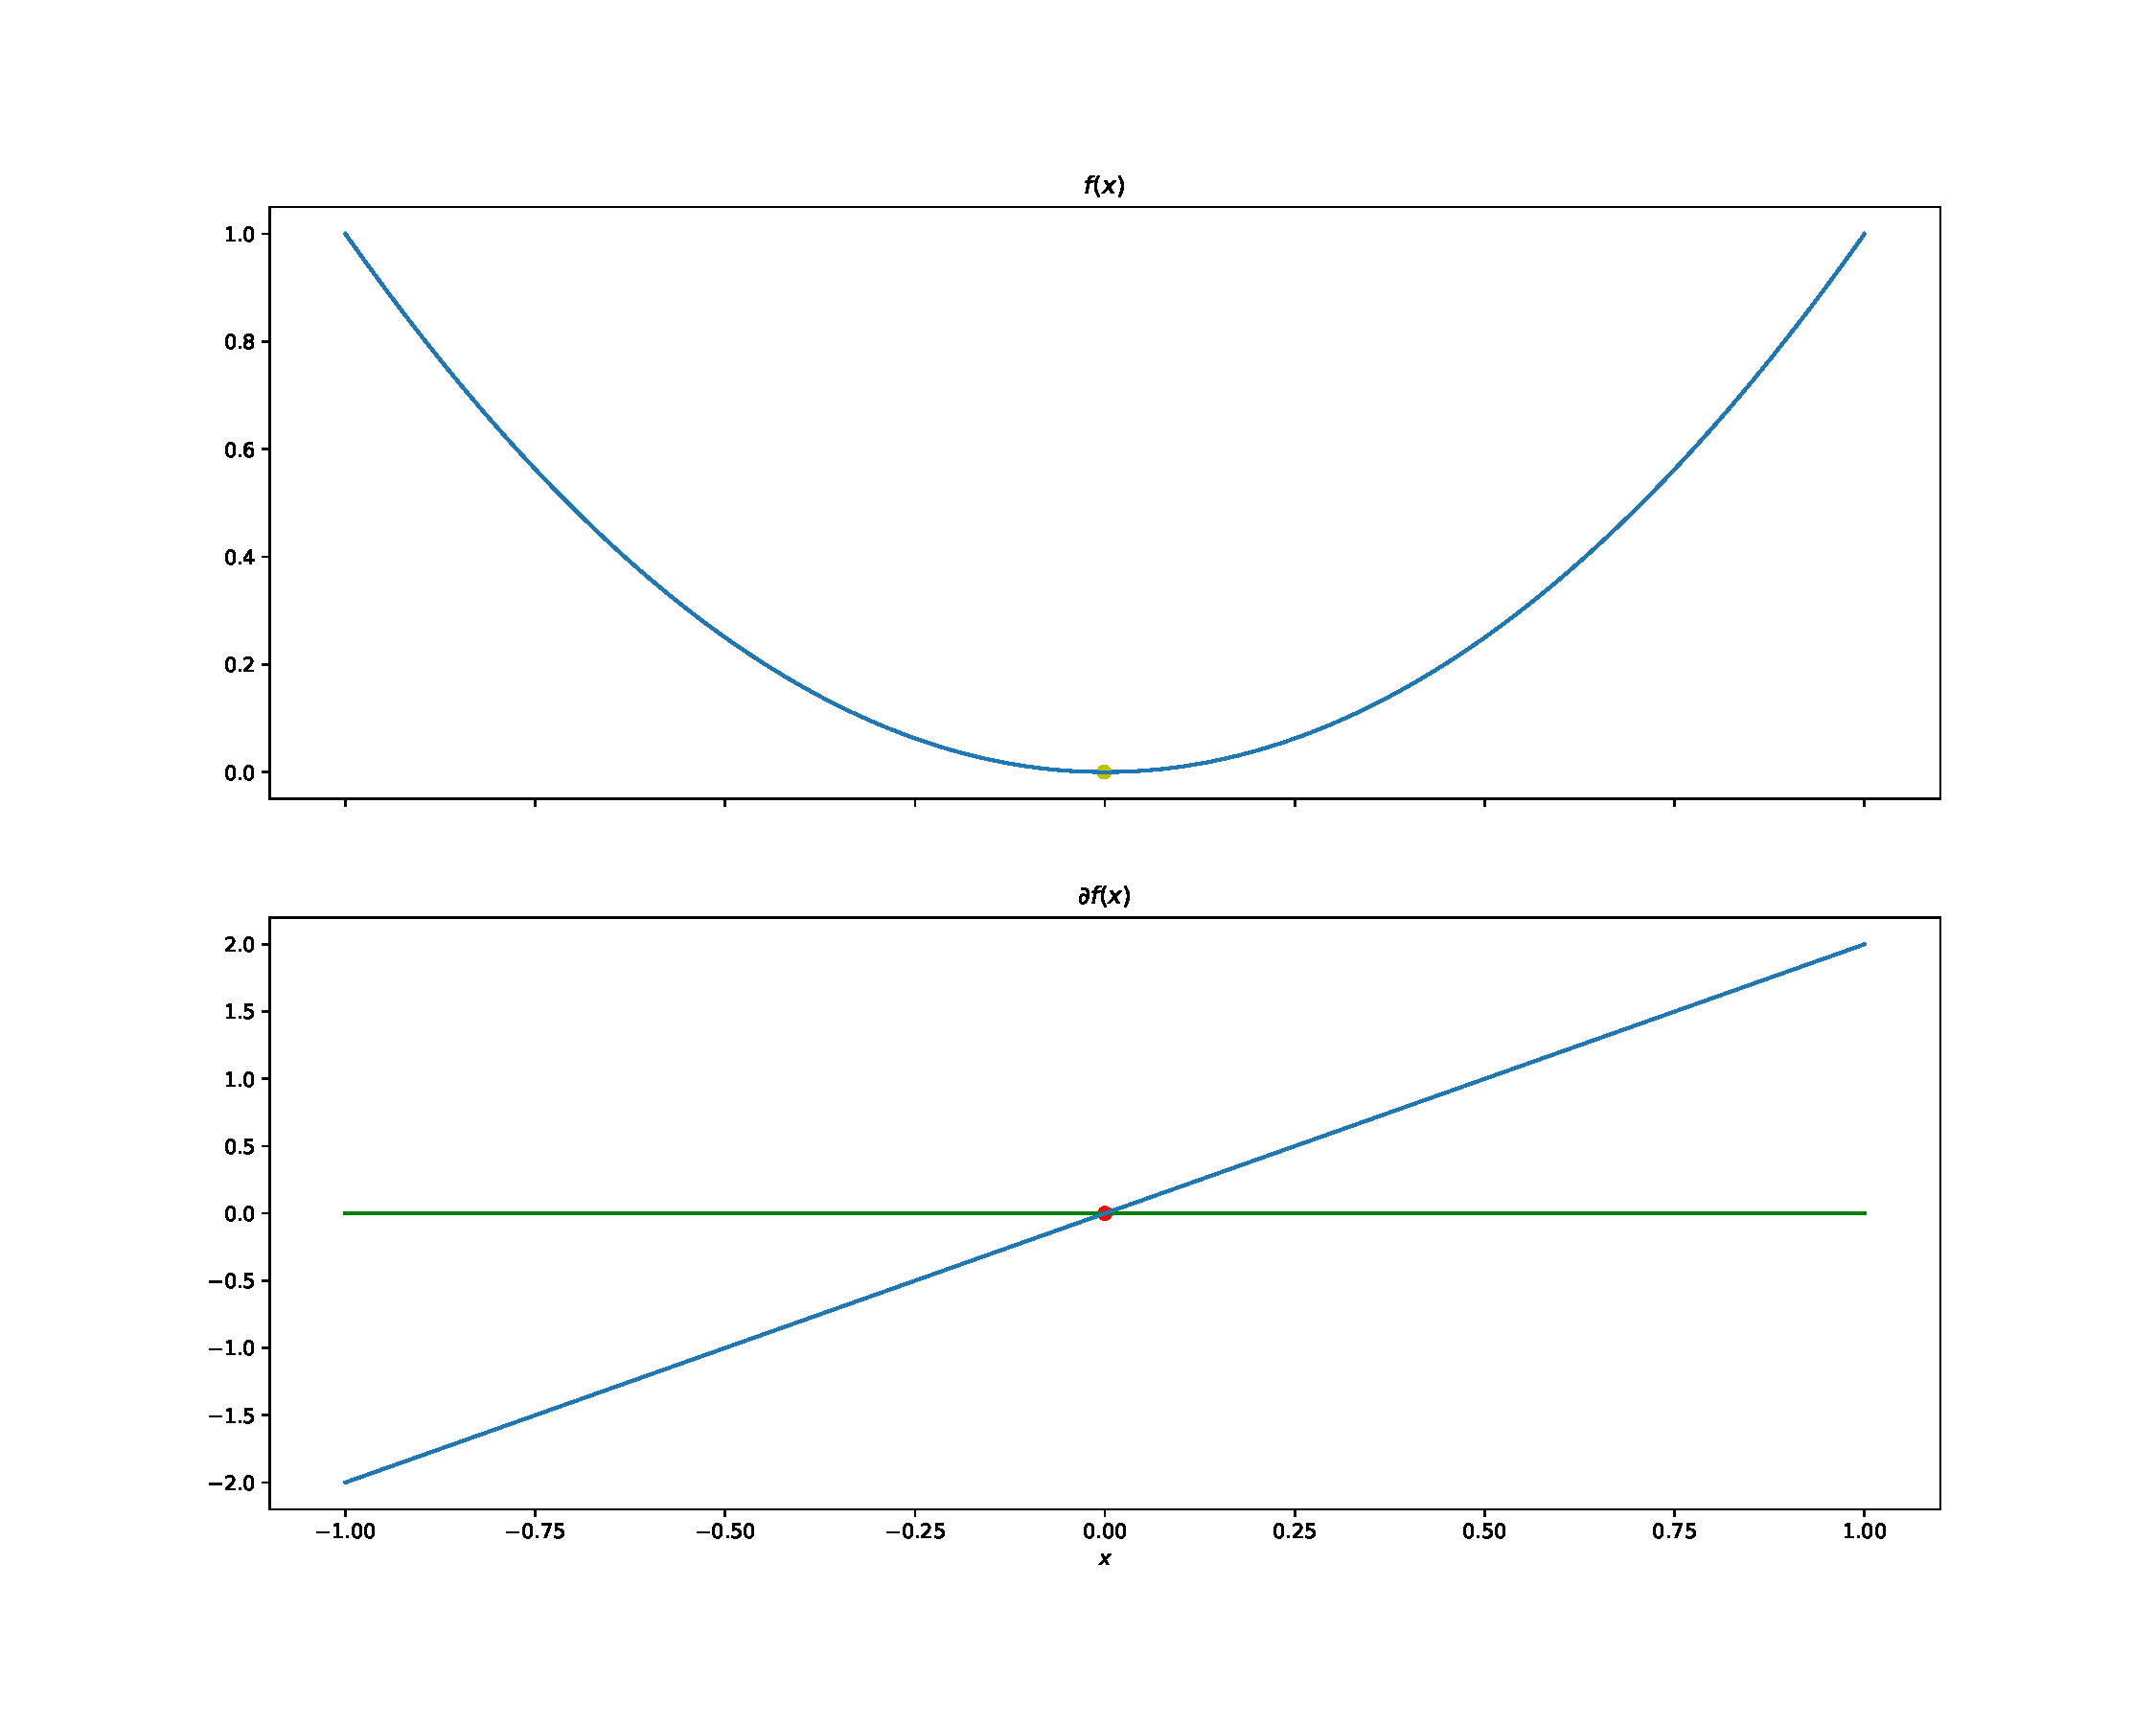
\includegraphics[width=\textwidth]{Chapter4/NeuroCom2021/ejemplo1_mse.pdf}
    \caption{Squared value function (top) and its corresponding subgradient (bottom). The green line represents the $0$ constant function. The yellow dot indicates the point minimizing the function.}
    \label{fig:sq_loss}
\end{figure}
This is the simplest case, since the squared function,
$f(x) = x^2 ,$
is differentiable, and its derivative is 
$\nabla f(x) = 2x$; both are shown in Figure~\ref{fig:sq_loss}.
Using the formulation of~\eqref{eq:subproblem_lambda}, the training error corresponding to the squared loss is
\begin{equation}
    \label{eq:opt_sq}
    \argmin_{\lambda \in [0, 1]} \mathcal{J}(\lambda) = \sum_{i=1}^{\npertask} \left({\lambda c_i + d_i}\right)^2 .
\end{equation}
In this case, $\mathcal{J}(\lambda)$ is a differentiable function, and its derivative is 
\begin{equation}
    \nonumber
    \mathcal{J}'(\lambda) = \sum_{i=1}^\npertask 2 c_i (\lambda c_i + d_i) .
\end{equation}
Solving $\mathcal{J}'(\lambda)= 0$ results in
%
\begin{equation*}
\lambda' =  -\frac{\sum_{i=1}^{\npertask} d_i c_i }{\sum_{i=1}^{\npertask} (c_i)^2 } ,
\end{equation*}
and the optimum is hence $\lambda^* = \max(0, \min(1, \lambda'))$.
\begin{figure}[t!]
    \centering
    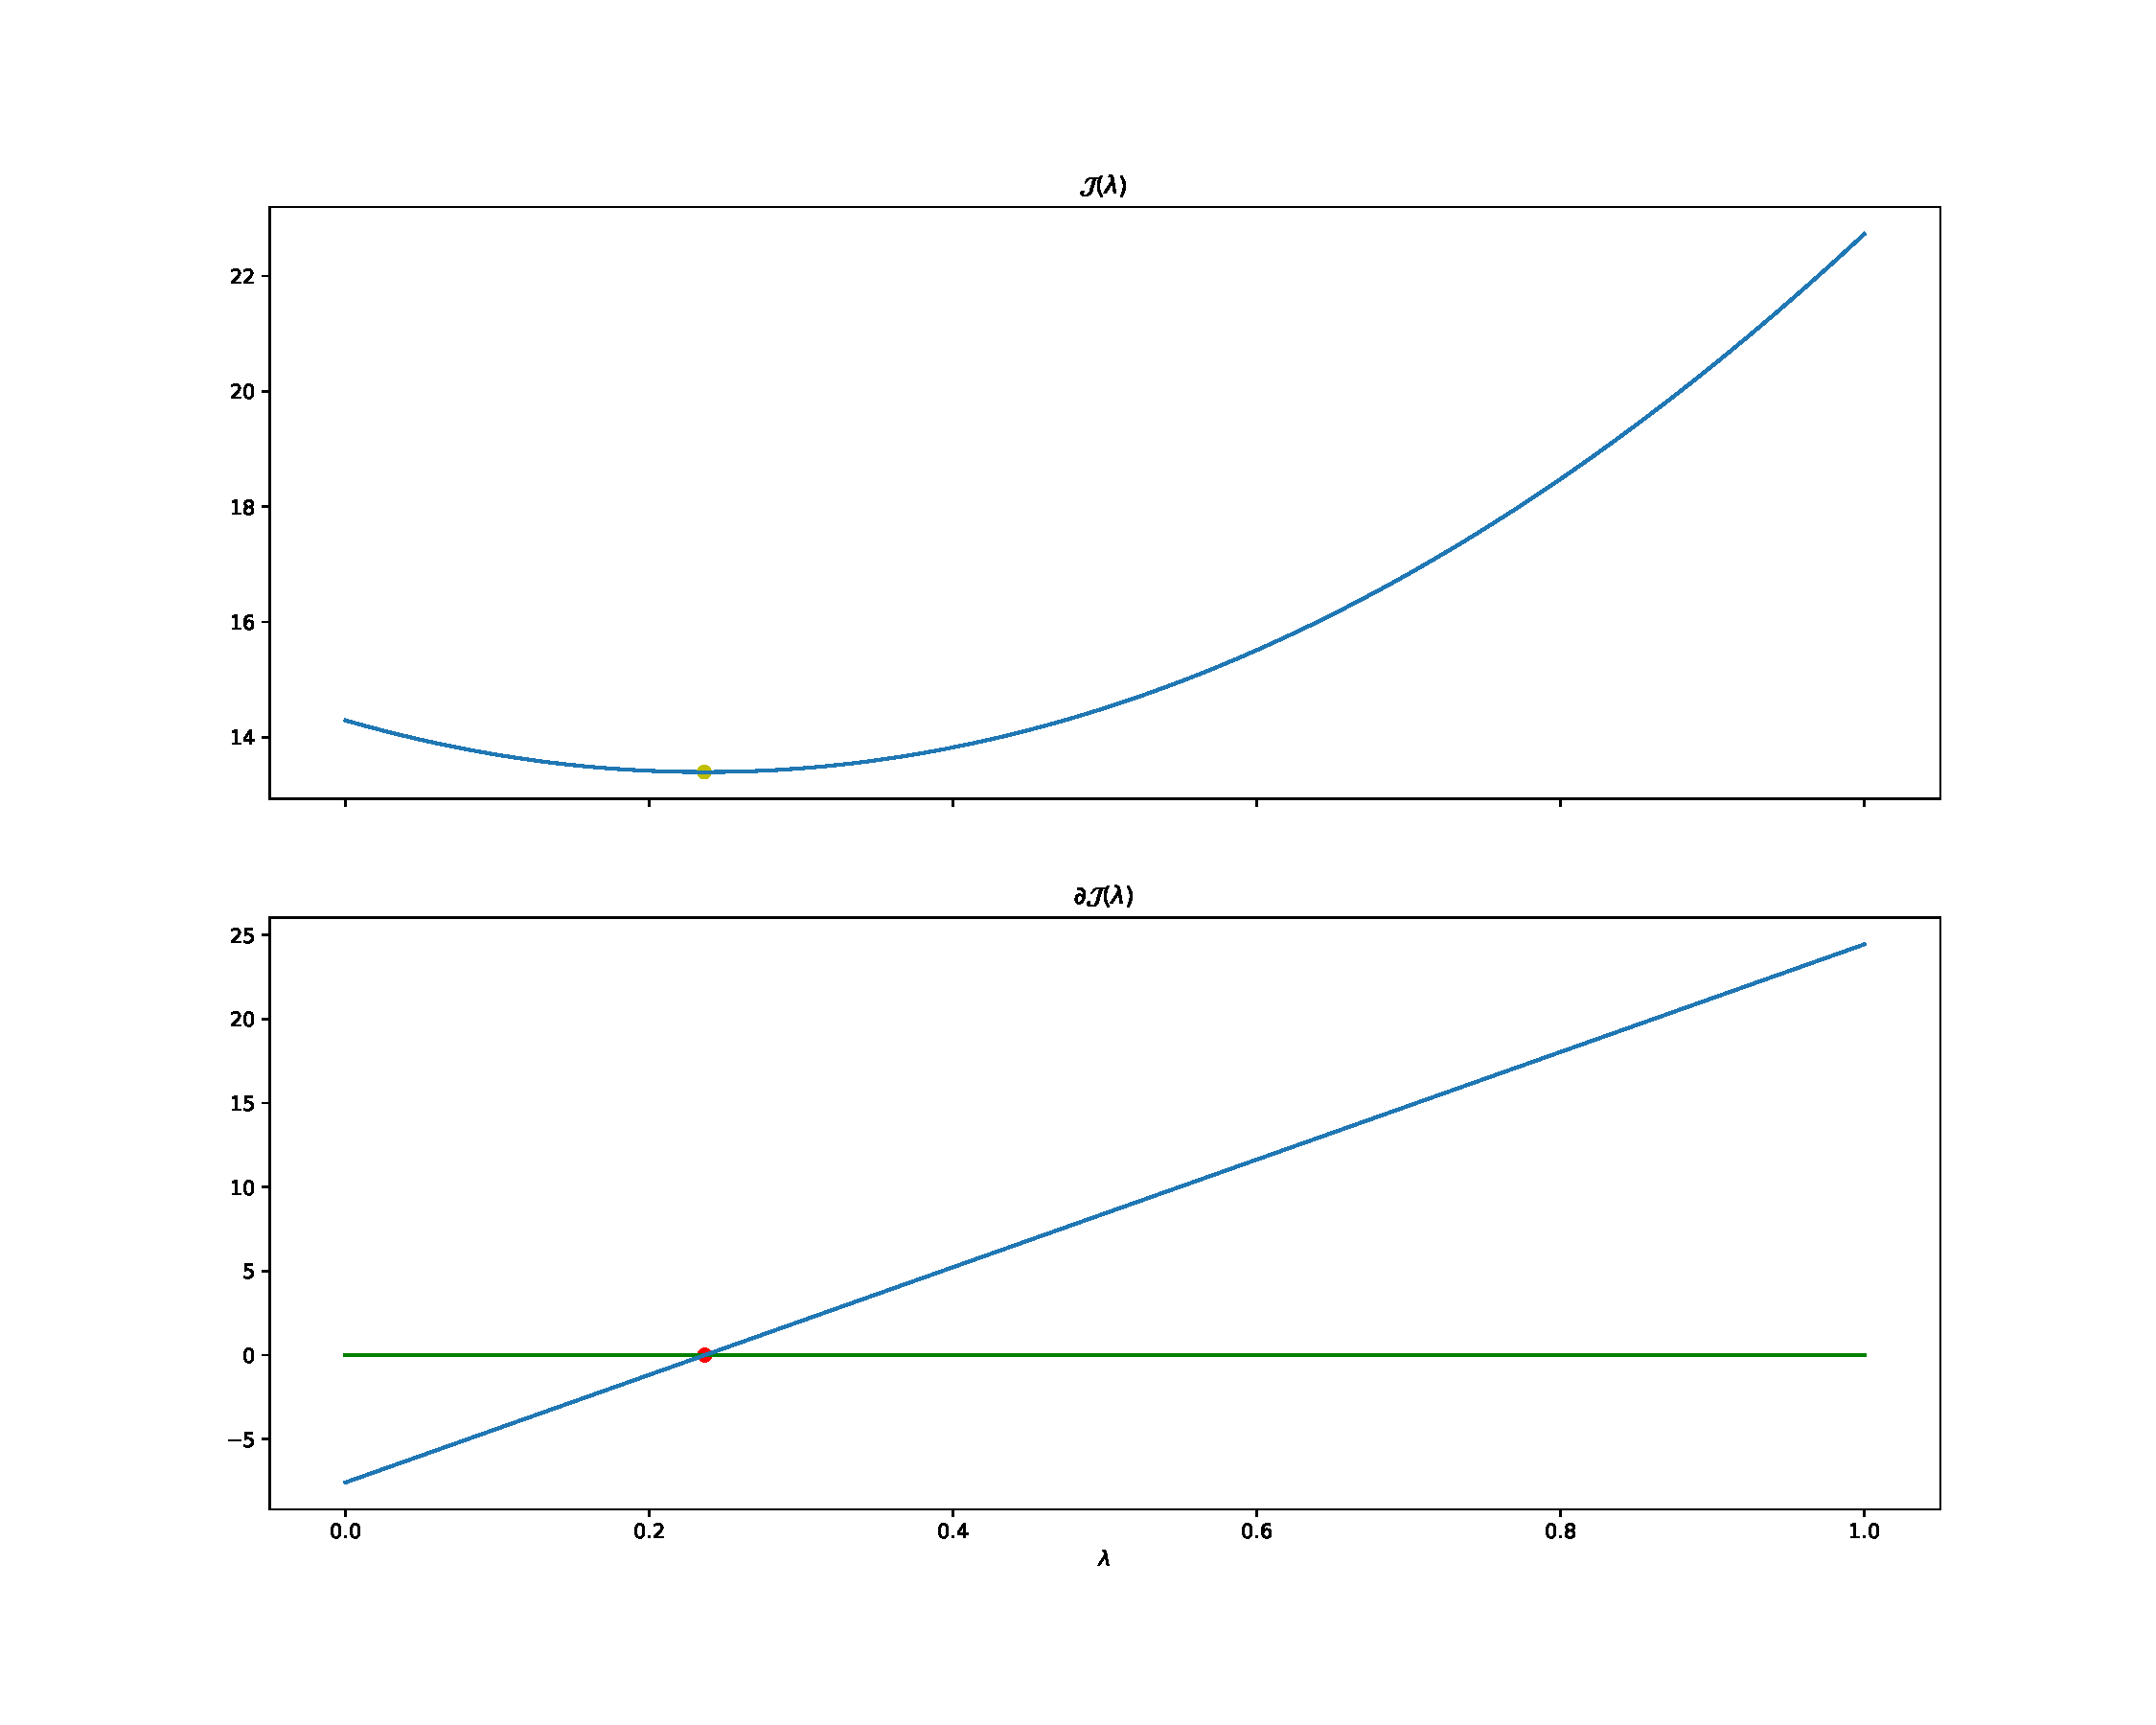
\includegraphics[width=\textwidth]{Chapter4/NeuroCom2021/ejemplo2_mse.pdf}
    \caption{Error using the squared loss function (top) and its corresponding subgradient (bottom). The green line represents the $0$ constant function. The yellow dot is the point minimizing the error, and whose corresponding subgradient contains the value $0$.}
    \label{fig:sq_error}
\end{figure}

In Figure~\ref{fig:sq_error} the error function using $10$ random pairs $(c_i, d_i)$ and its corresponding differential is shown.

\subsection{Absolute Loss}
\begin{figure}[t!]
    \centering
    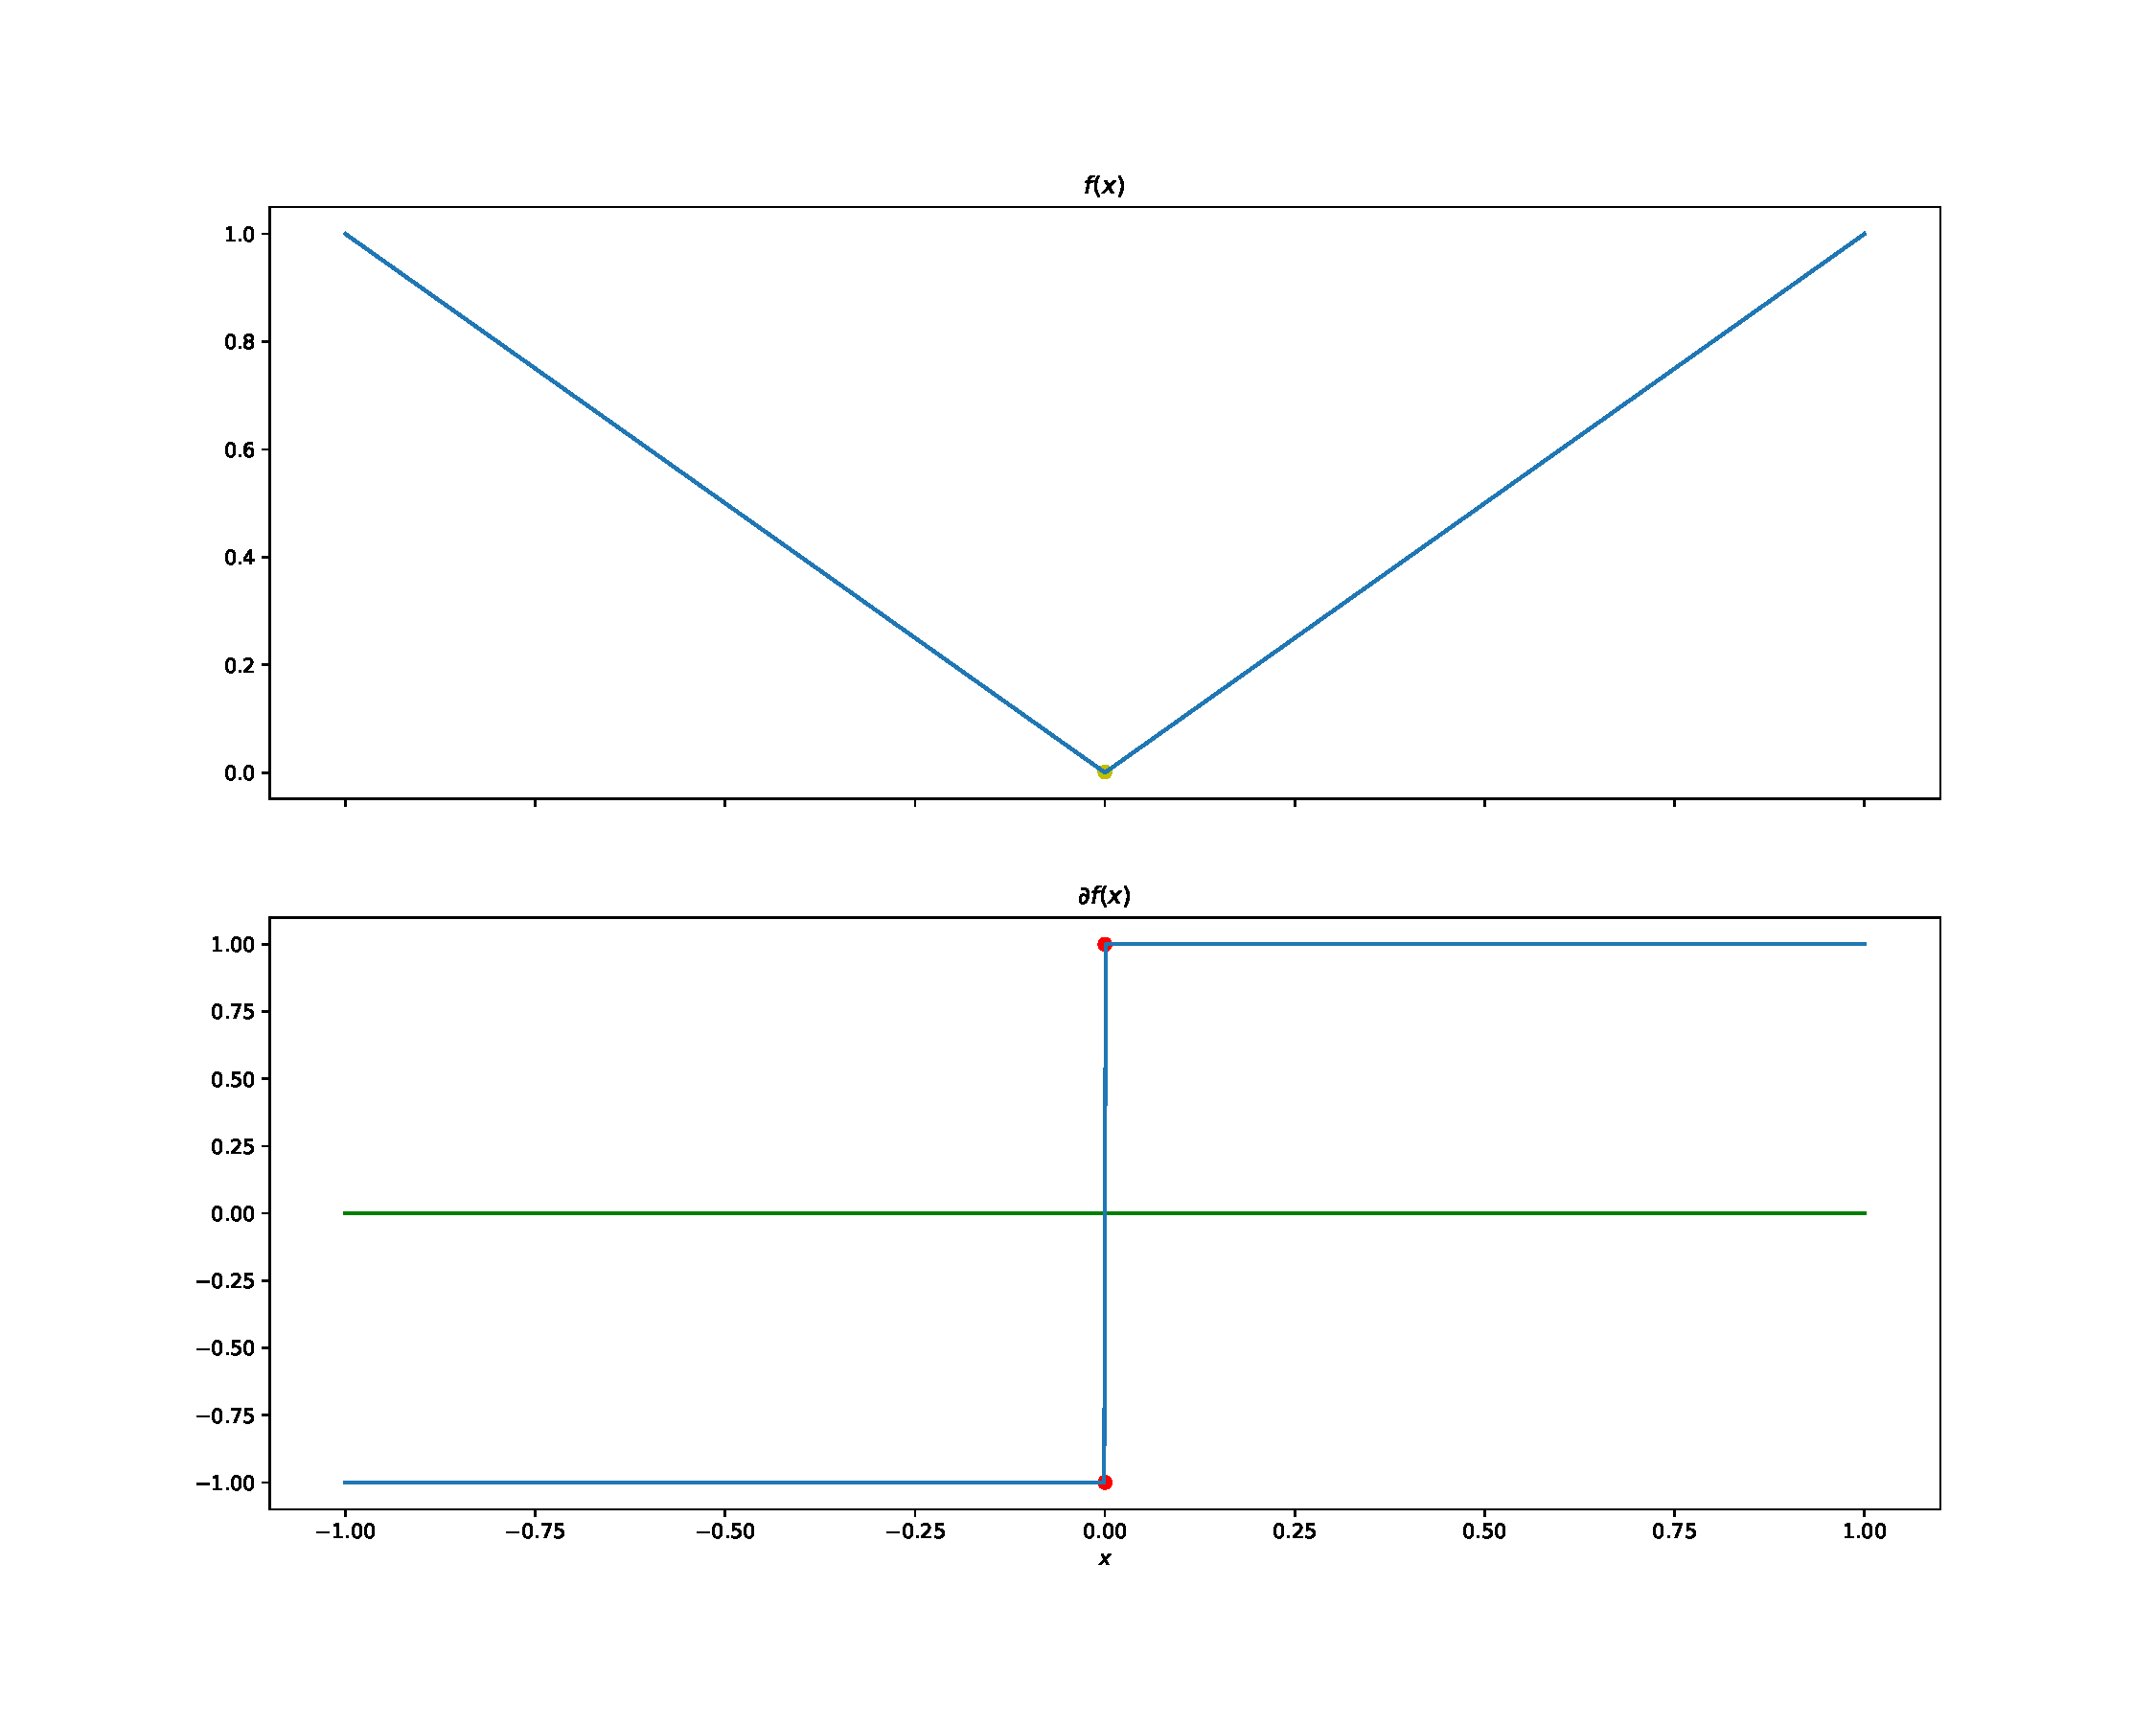
\includegraphics[width=\textwidth]{Chapter4/NeuroCom2021/ejemplo1_mae.pdf}
    \caption{Absolute value function (top) and its corresponding subgradient (bottom). The green line represents the $0$ constant function. The yellow dot indicates the point minimizing the function.}
    \label{fig:abs_loss}
\end{figure}
The absolute function 
\begin{equation}
    \nonumber
    f(x) = 
    \begin{cases}
    -x ,& x \leq 0, \\
    x ,& x > 0    
    \end{cases}
\end{equation}
is not differentiable at $0$, but the subgradient can be expressed at any point as
\begin{equation}
    \nonumber
    f(x) = 
    \begin{cases}
    -1 ,& x < 0, \\
    [-1, 1] ,& x = 0 , \\
    1 ,& x > 0 ,
    \end{cases}
\end{equation}
which is illustrated in Figure~\ref{fig:abs_loss}.
Using the formulation of~\eqref{eq:subproblem_lambda}, the training error corresponding to the absolute value loss is
\begin{equation}
    \label{eq:opt_abs}
    \argmin_{\lambda \in [0, 1]} \mathcal{J}(\lambda) = \sum_{i=1}^{\npertask} \abs{\lambda c_i + d_i}.
\end{equation}
Observe that in each term of the sum the subdifferential is 
\begin{equation}
    \label{eq:subdiff_abs}
    \begin{aligned}
        \partial \abs{\lambda c_i + d_i} = 
    \begin{cases}
        -\abs{c_i} ,& \lambda c_i + d_i  < 0, \\
        [-\abs{c_i}, \abs{c_i}] ,& \lambda c_i + d_i  = 0, \\
        \abs{c_i} ,& \lambda c_i + d_i  > 0 .\\
    \end{cases}
    \end{aligned}
\end{equation}
The elbows are obtained using the values $\frac{-d_i}{c_i}$, that can be clipped and sorted to get ${\lambda}_{(1)} < \ldots < {\lambda}_{(m)}$.
In~\citet[Proposition 2]{RuizAD21} we present the following result to get the optimal $\lambda^*$.
\begin{prop}[Optimal $\lambda^*$ with absolute value loss]\label{prop:abs_neurocom2020}
    In problem~\eqref{eq:opt_abs} $\lambda^*=0$ is optimal \emph{iff}
    \begin{equation}\nonumber
        - \sum_{i: \; 0 > \lambda_{(i)}} \abs{c_{(i)}} + \sum_{i: \; 0 < \lambda_{(i)}} \abs{c_{(i)}} \leq 0.
        \end{equation}
    If this condition does not hold, $\lambda^* \in (0,1)$ is optimal \emph{iff} $\lambda^*$ is a feasible elbow, that is, $0 < \lambda^* = \lambda_{(k)} < 1$ for some $k=1, \dotsc, \npertask$, and
    \begin{equation}\label{sol_abs_e}
    - \sum_{i:\; \lambda_{(k)} > \lambda_{(i)}} \abs{c_{(i)}} + \sum_{i:\; \lambda_{(k)} < \lambda_{(i)}} \abs{c_{(i)}} \in \left[ -  \abs{c_{(k)}},  \abs{c_{(k)}}  \right] .
    \end{equation}
    If none of the previous conditions hold, then $\lambda^*=1$ is optimal.
\end{prop}
\begin{proof}
    Observe in~\eqref{eq:subdiff_abs} that, for each term $\partial \abs{\lambda c_i + d_i}$, the change occurs at the elbow $\lambda_{i} = - d_ i / c_i$. We can consider two cases:
    \begin{itemize}
        \item $0 > c_i$, then
        \begin{equation}
            \nonumber
            \begin{aligned}
                \partial \abs{\lambda c_i + d_i} = 
            \begin{cases}
                -{c_i} ,& \lambda > \lambda_i, \\
                [-\abs{c_i}, \abs{c_i}] ,& \lambda = \lambda_i, \\
                {c_i} ,& \lambda < \lambda_i .\\
            \end{cases}
            \end{aligned}
        \end{equation}
        \item $0 < c_i$, then
        \begin{equation}
            \nonumber
            \begin{aligned}
                \partial \abs{\lambda c_i + d_i} = 
            \begin{cases}
                -{c_i} ,& \lambda < \lambda_i, \\
                [-\abs{c_i}, \abs{c_i}] ,& \lambda = \lambda_i, \\
                {c_i} ,& \lambda > \lambda_i .\\
            \end{cases}
            \end{aligned}
        \end{equation}
    \end{itemize}
    Consider the sorted elbow values $\lambda_{(1)}, \ldots, \lambda_{(m)}$.
    Recall that, since all functions share the same domain, the gradient of the sum is the gradient sum of the gradients, then, for $\lambda \neq \lambda_{(i)}$ for all $i=1,\ldots,\npertask$,
    \begin{equation}\nonumber
        \begin{aligned}
            \partial \mathcal{J}(\lambda) &=  \sum_{\substack{i:\; 0 > c_{(i)},\\ \;\; \lambda < \lambda_{(i)}}} {c_{(i)}} - \sum_{\substack{i:\; 0 > c_{(i)},\\ \;\; \lambda > \lambda_{(i)}}} {c_{(i)}}  - \sum_{\substack{i:\; 0 < c_{(i)},\\ \;\; \lambda < \lambda_{(i)}}} {c_{(i)}} + \sum_{\substack{i:\; 0 < c_{(i)},\\ \;\; \lambda > \lambda_{(i)}}} {c_{(i)}}   \\
            &= - \sum_{i: \; \lambda < \lambda_{(i)}} \sign(c_{(i)}) {c_{(i)}} + \sum_{i: \; \lambda > \lambda_{(i)}} \sign(c_{(i)}) {c_{(i)}} \\
            &= - \sum_{i: \; \lambda < \lambda_{(i)}} \abs{c_{(i)}} + \sum_{i: \; \lambda > \lambda_{(i)}} \abs{c_{(i)}} .
        \end{aligned}        
    \end{equation}
    We can highlight two factors here: the value of $\partial \mathcal{J}(\lambda)$ is constant between elbows, and $\partial \mathcal{J}(\lambda)$ is a non-decreasing function.
    Then, when $\lambda = \lambda_{(k)}$ for some $k=1, \ldots, \npertask$, we have that
    \begin{equation}
        \nonumber
        \partial \mathcal{J}(\lambda_{(k)}) = \left[ s_{(k)} - \abs{c_{(k)}}, s_{(k)} + \abs{c_{(k)}}   \right] ,
    \end{equation}
    where $s_{(k)} = - \sum_{i: \; \lambda_{(k)} < \lambda_{(i)}} c_{(i)} + \sum_{i: \; \lambda_{(k)} > \lambda_{(i)}} c_{(i)}.$
    Moreover, in $(\lambda_{(k-1)}, \lambda_{(k+1)})$, the value of the subdifferential is
    \begin{equation}
        \nonumber
        \partial \mathcal{J}(\lambda) = \begin{cases}
            s_{(k)} - \abs{c_{(k)}},& \lambda < \lambda_{(k)}\\
            \left[ s_{(k)} - \abs{c_{(k)}}, s_{(k)} + \abs{c_{(k)}}   \right],& \lambda = \lambda_{(k)} \\
            s_{(k)} + \abs{c_{(k)}},& \lambda > \lambda_{(k)}
        \end{cases} .
    \end{equation}
    That is, $\partial \mathcal{J}(\lambda)$ is continuous, non-decreasing, and the values of the subdifferential between elbows are contained in the elbows subdifferential, thus, it is sufficient to look for the optimal value at the elbows.
    Then, using the Fermat rule, we want to find $\lambda^*$ such that $\partial \mathcal{J}(\lambda^*) = 0$. We have three possible scenarios:
    \begin{itemize}
        \item $\partial \mathcal{J}(0) \geq 0.$ 
        \\Since $\partial \mathcal{J}(\lambda)$ is non-decreasing, the optimal value in $[0, 1]$ is $\lambda^* = 0$.
        \item $0 \in \left[ s_{(k)} - \abs{c_{(k)}}, s_{(k)} + \abs{c_{(k)}}   \right] = \partial \mathcal{J}(\lambda_{(k)}), \; 0 < \lambda_{(k)} < 1$ for some $k=1, \ldots, \npertask$. 
        \\Then, the optimal value is $\lambda^*=\lambda_{(k)}$.
        \item $\partial \mathcal{J}(1) \leq 0$. 
        \\None of the previous conditions hold, and since $\partial \mathcal{J}(\lambda)$ is non-decreasing, the optimal value in $[0, 1]$ is $\lambda^* = 1$.
    \end{itemize}
\end{proof}
\begin{figure}[t!]
    \centering
    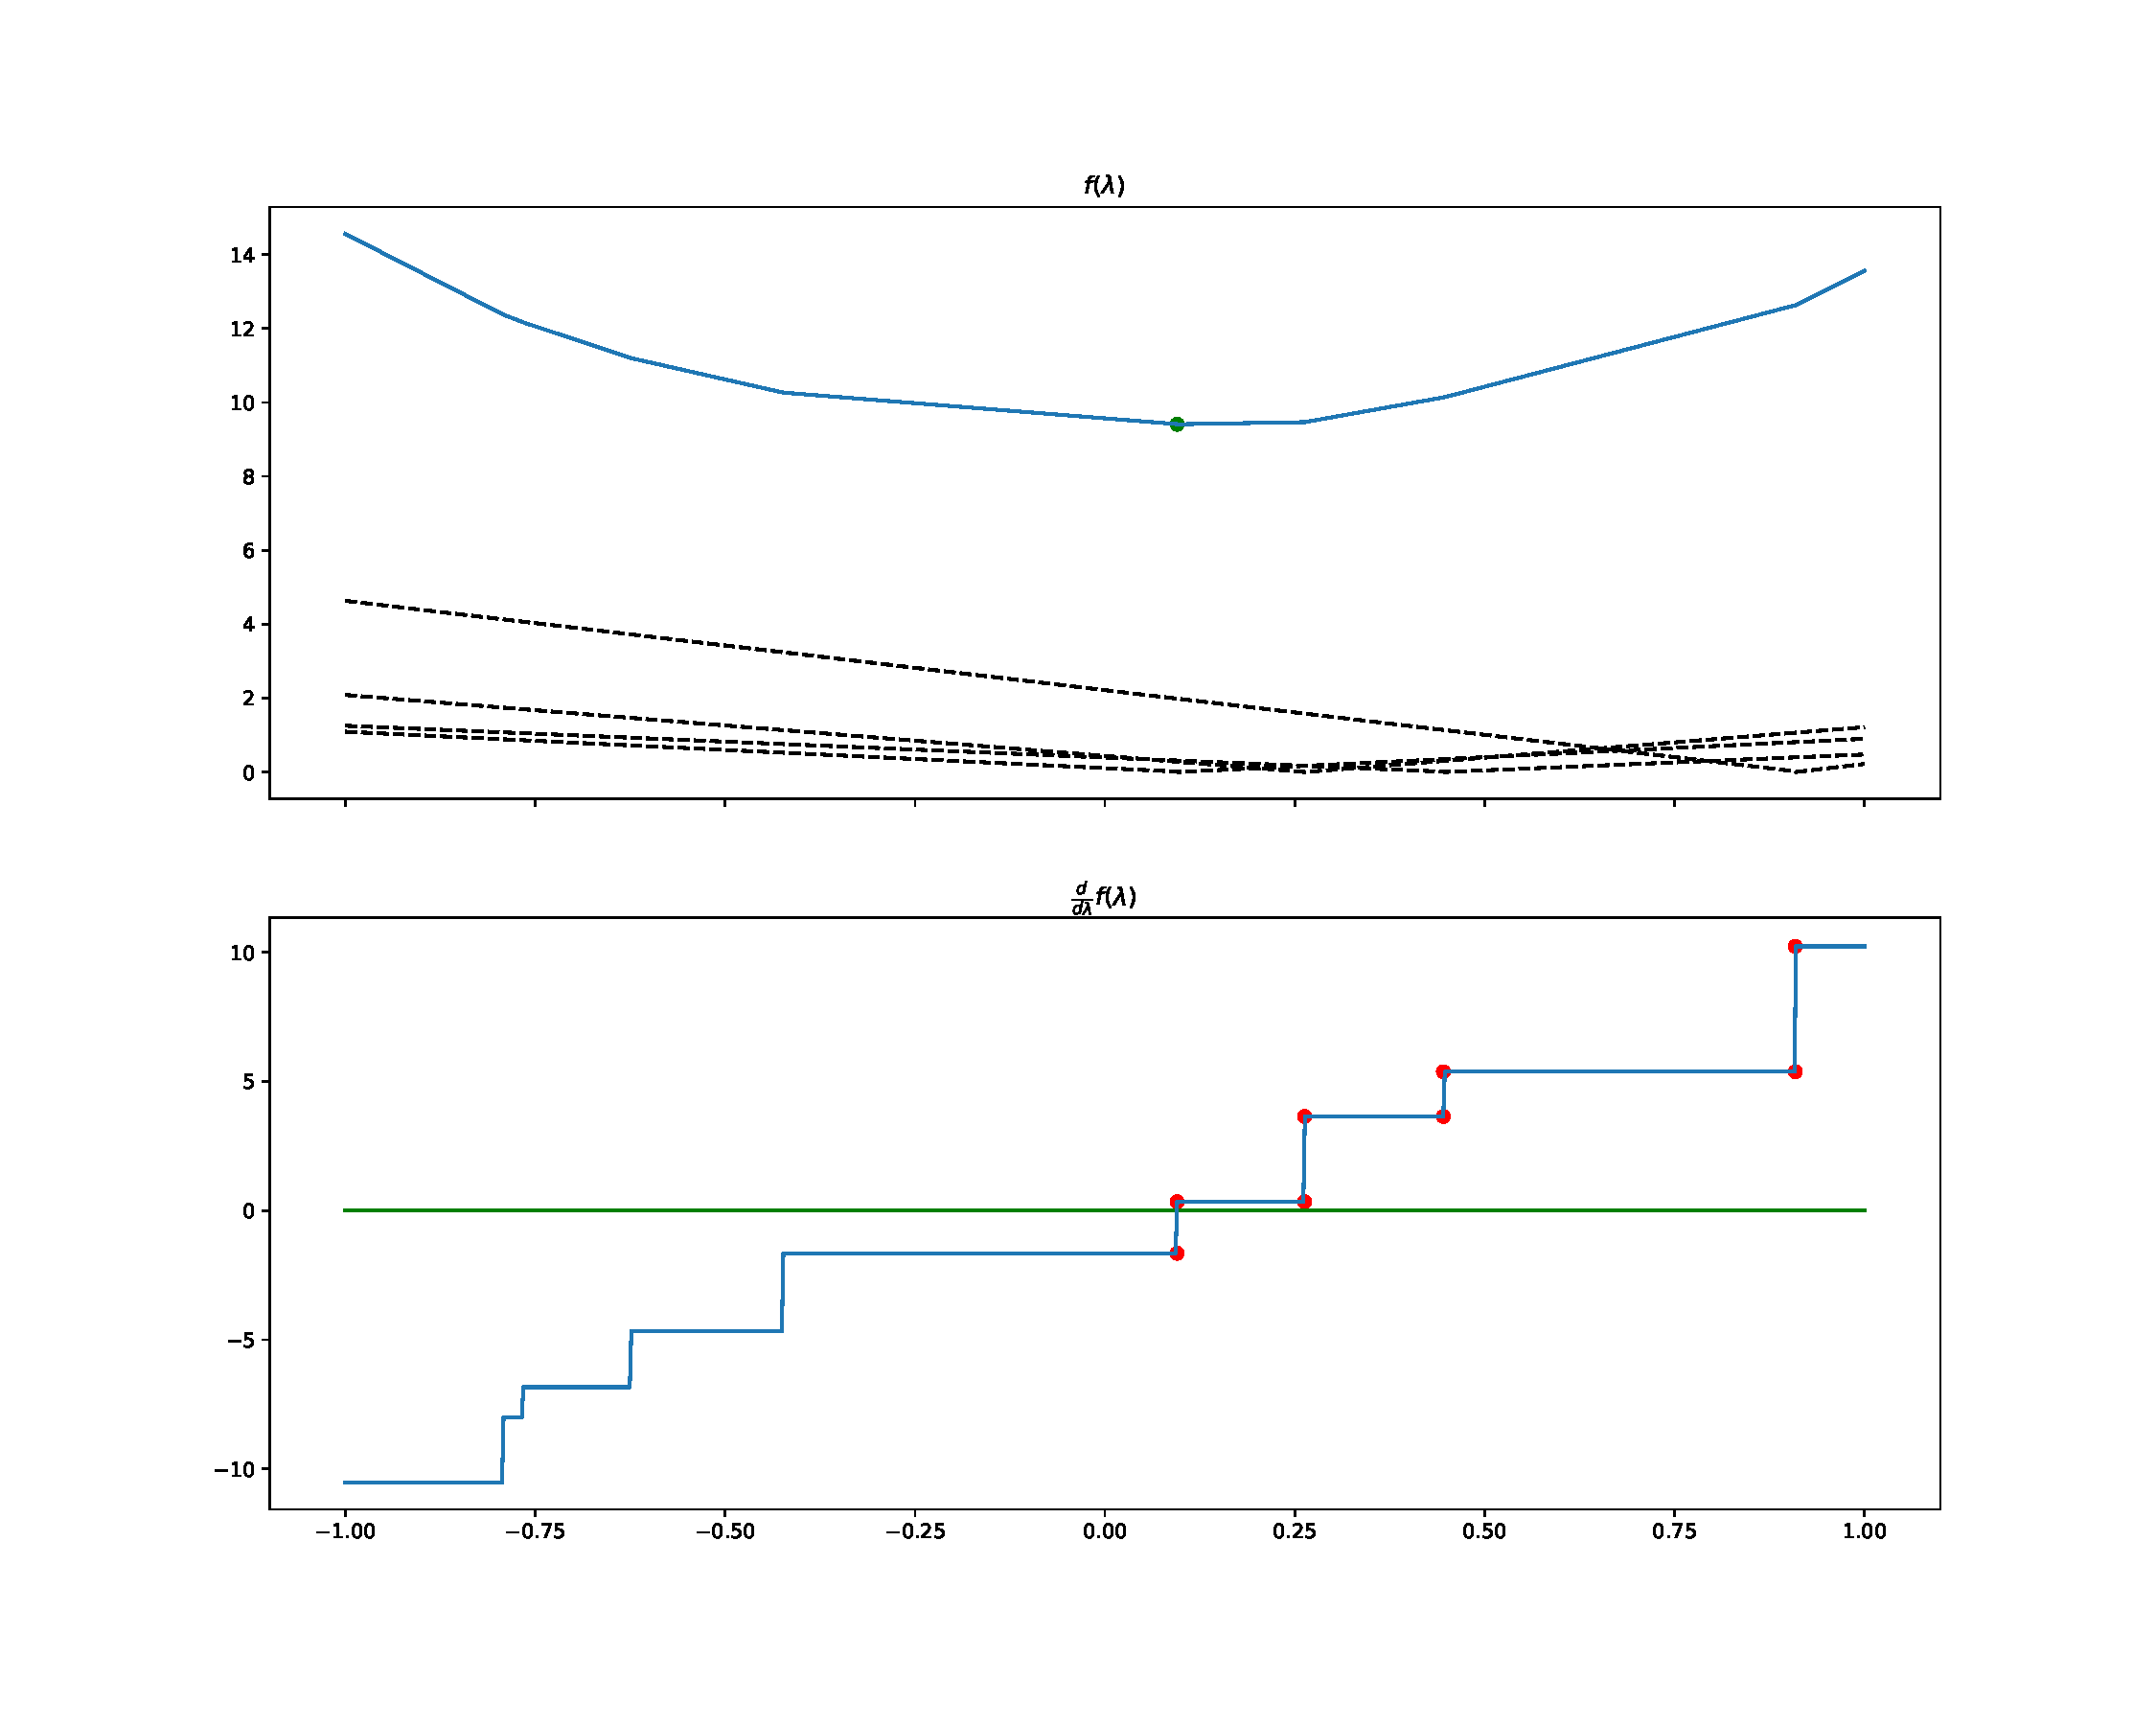
\includegraphics[width=\textwidth]{Chapter4/NeuroCom2021/ejemplo2_mae.pdf}
    \caption{Error using the absolute loss function (top) and its corresponding subgradient (bottom). The green line represents the $0$ constant function. Red dots mark the extremes of the subdifferential intervals of non-differentiable points. The yellow dot is the point minimizing the error, and whose corresponding subgradient contains the value $0$.}
    \label{fig:abs_error}
\end{figure}
The meaning of this proposition is depicted in Figure~\ref{fig:abs_error}, where the error and its corresponding subgradient is computed for $10$ random pairs $(c_i, d_i)$. It can be seen that the subdifferential is constant between elbows, and takes a step at the elbows. Then, the parameter $\lambda^*$ is optimal when $0 \in \partial J(\lambda^*)$.

Observe that, once the elbows are sorted, the cost of computing the optimal value $\lambda^*$ is linear, since we just have to compute the quantities $s_{(k)}$ for $k=1, \ldots, \npertask$, and $s_{(k+1)} = s_{(k)} + 2 \abs{c_{(k)}}$  for each $k$. At each step, we check the optimality condition $0 \in [s_{(k)} - \abs{c_{(k)}}, s_{(k)} + \abs{c_{(k)}}]$.
Thus, the bottleneck of the procedure is sorting the elbows, which supposes an average cost of $O(\npertask \log(\npertask))$.


\subsection{Hinge Loss}
The positive part function 
\begin{equation}
    \nonumber
    f(x) = 
    \begin{cases}
    0 ,& x \leq 0, \\
    x ,& x > 0    
    \end{cases}
\end{equation}
is not differentiable at $0$, but, again, the subgradient can be expressed at any point as
\begin{equation}
    \nonumber
    f(x) = 
    \begin{cases}
    0 ,& x < 0, \\
    [0, 1] ,& x = 0 , \\
    1 ,& x > 0 ,
    \end{cases}
\end{equation}
which is illustrated in Figure~\ref{fig:hinge_loss}.
\begin{figure}[t!]
    \centering
    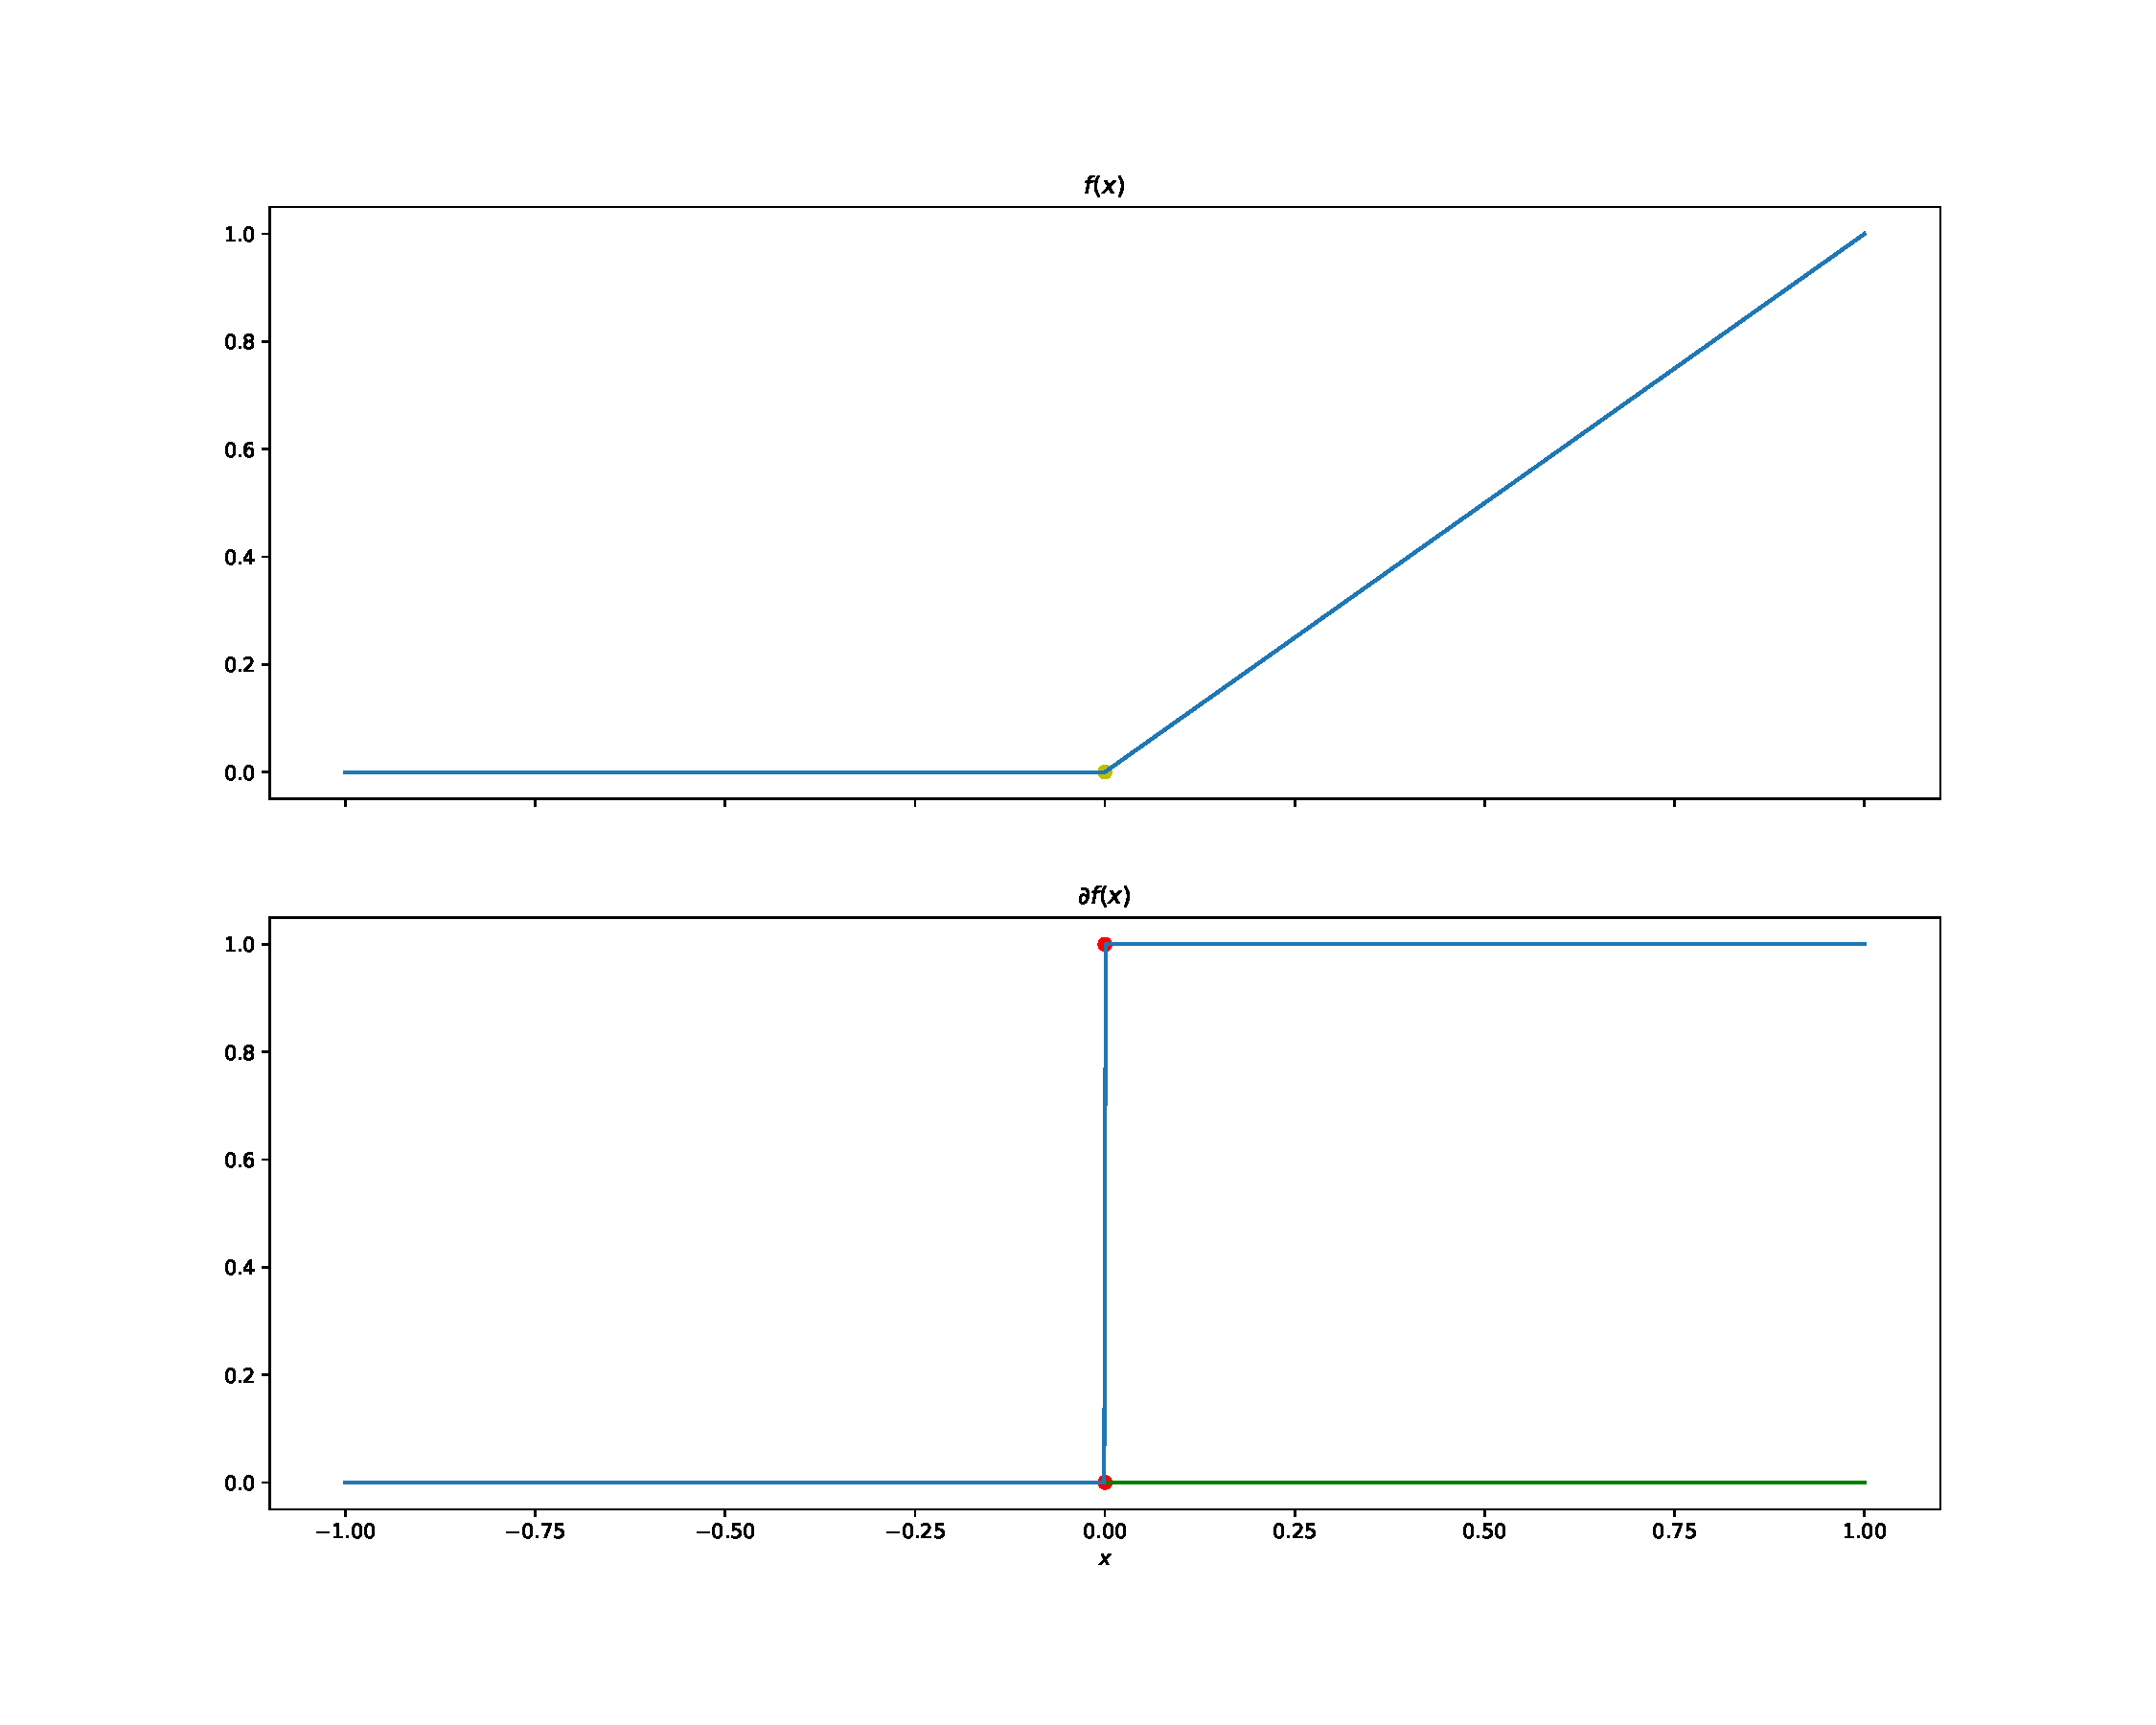
\includegraphics[width=\textwidth]{Chapter4/NeuroCom2021/ejemplo1_hinge.pdf}
    \caption{Positive part function (top) and its corresponding subgradient (bottom). The green line represents the $0$ constant function. The yellow dot indicates the point minimizing the function.}
    \label{fig:hinge_loss}
\end{figure}
Using the formulation of~\eqref{eq:subproblem_lambda}, the training error corresponding to the hinge loss is
\begin{equation}
    \label{eq:opt_hinge_l1}
    \argmin_{\lambda \in [0, 1]} \mathcal{J}(\lambda) = \sum_{i=1}^{\npertask} \pospart{\lambda c_i + d_i}.
\end{equation}
Observe that in each term of the sum the subdifferential is 
\begin{equation}
    \label{eq:subdiff_hinge_l1}
    \begin{aligned}
        \partial \left[\lambda c_i + d_i \right]_+ = 
    \begin{cases}
        0 ,& \lambda c_i + d_i  < 0, \\
        [\min(0, c_i), \max(0, c_i)] ,& \lambda c_i + d_i  = 0, \\
        c_i ,& \lambda c_i + d_i  > 0. \\
    \end{cases}
    \end{aligned}
\end{equation}
That is, the elbows are related to the values $\frac{-d_i}{c_i}$, that can be clipped and sorted to obtain the elbows ${\lambda}_{(1)} < \ldots < {\lambda}_{(m)}$.
In~\citet[Proposition 2]{RuizAD21} we present the following result to get the optimal $\lambda^*$.
\begin{prop}[Optimal $\lambda^*$ with hinge loss]\label{prop:hinge_neurocom2020}
    In~\eqref{eq:opt_hinge_l1}, $\lambda^*=0$ is optimal iff
    \begin{equation}\label{eq:sol_hinge_0}
        -\sum_{i:\; 0 > \lambda_{(i)}} \mymax{0, c_{(i)}} - \sum_{0 < \lambda_{(i)}} \mymin{0, c_{(i)}} \leq 0 .
        \end{equation}
        If this condition does not hold, a value $\lambda^* \in (0, 1)$ is optimal for problem~\eqref{eq:opt_hinge_l1} \emph{iff} $\lambda^*$ is a feasible elbow, that is, $0 < \lambda^* = \lambda_{(k)} < 1$ for some $k=1, \dotsc, \npertask$, and
    \begin{equation}\label{eq:sol_hinge}
        -\sum_{i:\; \lambda_{(k)} > \lambda_{(i)}} \mymax{0, c_{(i)}} - \sum_{i:\; \lambda_{(k)} <\lambda_{(i)}} \mymin{0, c_{(i)}} \in \left[\mymin{0, c_{(k)}}, \mymax{0, c_{(k)}} \right] .
    \end{equation}
    If none of the previous conditions hold, then $\lambda^*=1$ is optimal.
\end{prop}
\begin{proof}
    Observe in~\eqref{eq:subdiff_hinge_l1} that, for each term $\partial \abs{\lambda c_i + d_i}$, the change occurs at the elbow $\lambda_{i} = - d_ i / c_i$. We can consider two cases:
    \begin{itemize}
        \item $0 > c_i$, then
        \begin{equation}
            \nonumber
            \begin{aligned}
                \partial \pospart{\lambda c_i + d_i} = 
            \begin{cases}
                0 ,& \lambda > \lambda_i, \\
                [\min(0, c_i), \max(0, c_i)] ,& \lambda = \lambda_i, \\
                {c_i} ,& \lambda < \lambda_i .\\
            \end{cases}
            \end{aligned}
        \end{equation}
        \item $0 < c_i$, then
        \begin{equation}
            \nonumber
            \begin{aligned}
                \partial \pospart{\lambda c_i + d_i} = 
            \begin{cases}
                0 ,& \lambda < \lambda_i, \\
                [\min(0, c_i), \max(0, c_i)] ,& \lambda = \lambda_i, \\
                {c_i} ,& \lambda > \lambda_i .\\
            \end{cases}
            \end{aligned}
        \end{equation}
    \end{itemize}
    Consider the sorted elbow values $\lambda_{(1)}, \ldots, \lambda_{(m)}$.
    Recall that, since all functions share the same domain, the gradient of the sum is the gradient sum of the gradients, then, for $\lambda \neq \lambda_{(i)}$ for all $i=1,\ldots,\npertask$,
    \begin{equation}\nonumber
        \begin{aligned}
            \partial \mathcal{J}(\lambda) &=  \sum_{\substack{i:\; 0 > c_{(i)},\\ \;\; \lambda < \lambda_{(i)}}} {c_{(i)}} + \sum_{\substack{i:\; 0 < c_{(i)},\\ \;\; \lambda > \lambda_{(i)}}} {c_{(i)}}  = \sum_{i: \; \lambda < \lambda_{(i)}} \mymin{0, c_{(i)}} + \sum_{i: \; \lambda > \lambda_{(i)}} \mymax{0, c_{(i)}}
        \end{aligned}        
    \end{equation}
    We can highlight two factors here: the value of $\partial \mathcal{J}(\lambda)$ is constant between elbows, and $\partial \mathcal{J}(\lambda)$ is a non-decreasing function.
    Then, when $\lambda = \lambda_{(k)}$ for some $k=1, \ldots, \npertask$, we have that
    \begin{equation}
        \nonumber
        \partial \mathcal{J}(\lambda_{(k)}) = \left[ s_{(k)} + \mymin{0, c_{(k)}}, s_{(k)} + \mymax{0, c_{(k)}}  \right] ,
    \end{equation}
    where $s_{(k)} = \sum_{i: \; \lambda_{(k)} < \lambda_{(i)}} \mymin{0, c_{(i)}} + \sum_{i: \; \lambda_{(k)} > \lambda_{(i)}} \mymax{0, c_{(i)}}.$
    Moreover, in $(\lambda_{(k-1)}, \lambda_{(k+1)})$, the value of the subdifferential is
    \begin{equation}
        \nonumber
        \partial \mathcal{J}(\lambda) = \begin{cases}
            s_{(k)} + \mymin{0, c_{(k)}},& \lambda < \lambda_{(k)}\\
            \left[ s_{(k)} + \mymin{0, c_{(k)}}, s_{(k)} + \mymax{0, c_{(k)}}   \right],& \lambda = \lambda_{(k)} \\
            s_{(k)} + \mymax{0, c_{(k)}},& \lambda > \lambda_{(k)}
        \end{cases} .
    \end{equation}
    That is, $\partial \mathcal{J}(\lambda)$ is continuous, non-decreasing, and the values between elbows are contained in the elbows subdifferential, thus, it is sufficient to look for the optimal value at the elbows.
    Then, using the Fermat rule, we want to find $\lambda^*$ such that $\partial \mathcal{J}(\lambda^*) = 0$. We have three possible scenarios:
    \begin{itemize}
        \item $\partial \mathcal{J}(0) \geq 0.$ 
        \\Since $\partial \mathcal{J}(\lambda)$ is non-decreasing, the optimal value in $[0, 1]$ is $\lambda^* = 0$.
        \item $0 \in \left[ s_{(k)} + \mymin{0, c_{(k)}}, s_{(k)} + \mymax{0, c_{(k)}}   \right] = \partial \mathcal{J}(\lambda_{(k)}), \; 0 < \lambda_{(k)} < 1$ for some $k=1, \ldots, \npertask$. 
        \\Then, the optimal value is $\lambda^*=\lambda_{(k)}$.
        \item $\partial \mathcal{J}(1) \leq 0$. 
        \\None of the previous conditions hold, and since $\partial \mathcal{J}(\lambda)$ is non-decreasing, the optimal value in $[0, 1]$ is $\lambda^* = 1$.
    \end{itemize}
\end{proof}
\begin{figure}[t!]
    \centering
    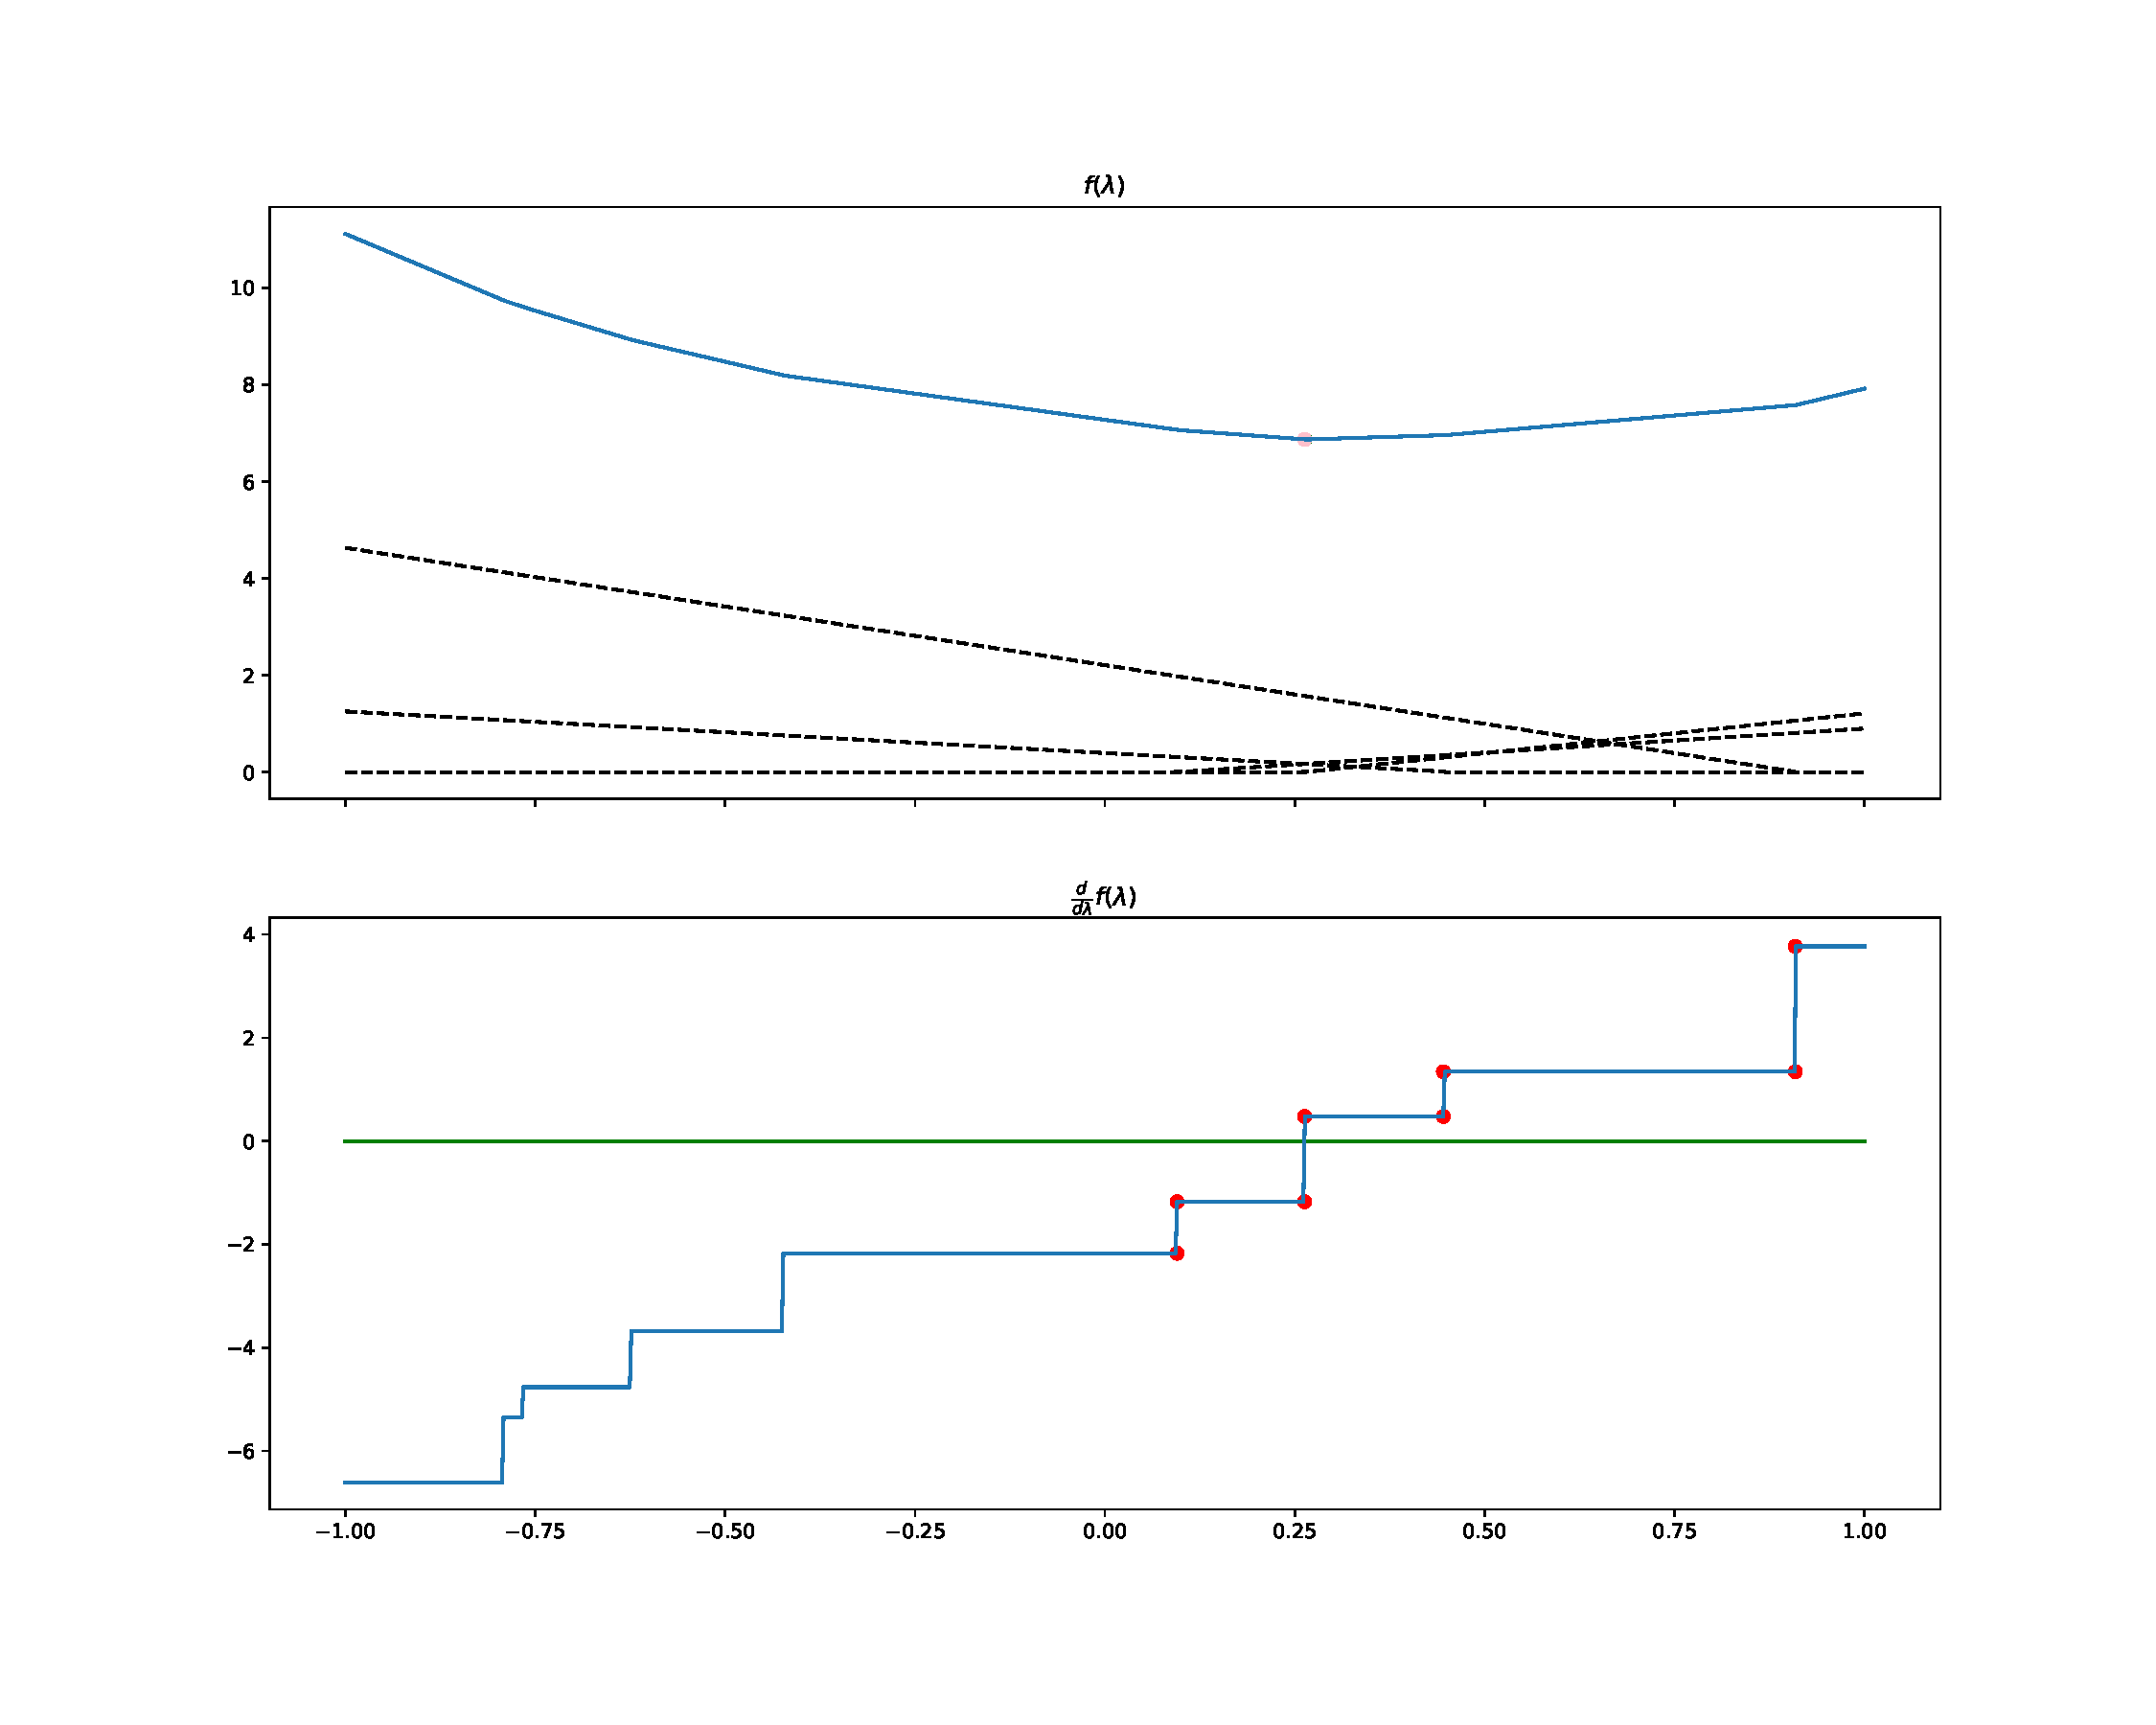
\includegraphics[width=\textwidth]{Chapter4/NeuroCom2021/ejemplo2_hinge.pdf}
    \caption{Error using the hinge loss function (top) and its corresponding subgradient (bottom). The green line represents the $0$ constant function. Red dots mark the extremes of the subdifferential intervals of non-differentiable points. The yellow dot is the point minimizing the error, and whose corresponding subgradient contains the value $0$.}
    \label{fig:hinge_error}
\end{figure}

Again, the results of the proposition are illustrated in Figure~\ref{fig:hinge_error}, where $10$ pairs $(c_i, d_i)$ are randomly sampled, and the corresponding error function $\mathcal{J}(\lambda)$ and its subgradient are shown. Here, similarly to the absolute loss case, the subgradient is constant between elbows, and at each elbow $\lambda_{(k)}$ the subgradient is an interval.

As with the absolute loss, once the elbows are sorted, the cost of computing the optimal value $\lambda^*$ is linear, since we just have to compute the quantities $s_{(k)}$ for $k=1, \ldots, \npertask$, and now $s_{(k+1)} = s_{(k)} + \abs{c_{(k)}}$  for each $k$. At each step, we check the optimality condition $0 \in [s_{(k)} - \mymin{0, c_{(k)}}, s_{(k)} + \mymax{0, c_{(k)}}]$.
As before, the largest cost of the procedure is sorting the elbows, and it has an average cost of $O(\npertask \log(\npertask))$.

\subsection{Squared Hinge Loss}
The squared positive part function is
\begin{equation}
    \nonumber
    f(x) = 
    \begin{cases}
    0 ,& x \leq 0, \\
    x^2 ,& x > 0    .
    \end{cases}
\end{equation}
and its gradient can be expressed at any point as
\begin{equation}
    \nonumber
    f(x) = 
    \begin{cases}
    0 ,& x \leq 0, \\
    2x ,& x > 0 .
    \end{cases}
\end{equation}
which is illustrated in Figure~\ref{fig:hinge_loss}.
Although the gradient can be defined at any point, the definition by parts makes it difficult to get the optimal value $\lambda^*$ that minimizes the corresponding training error.
\begin{figure}[t!]
    \centering
    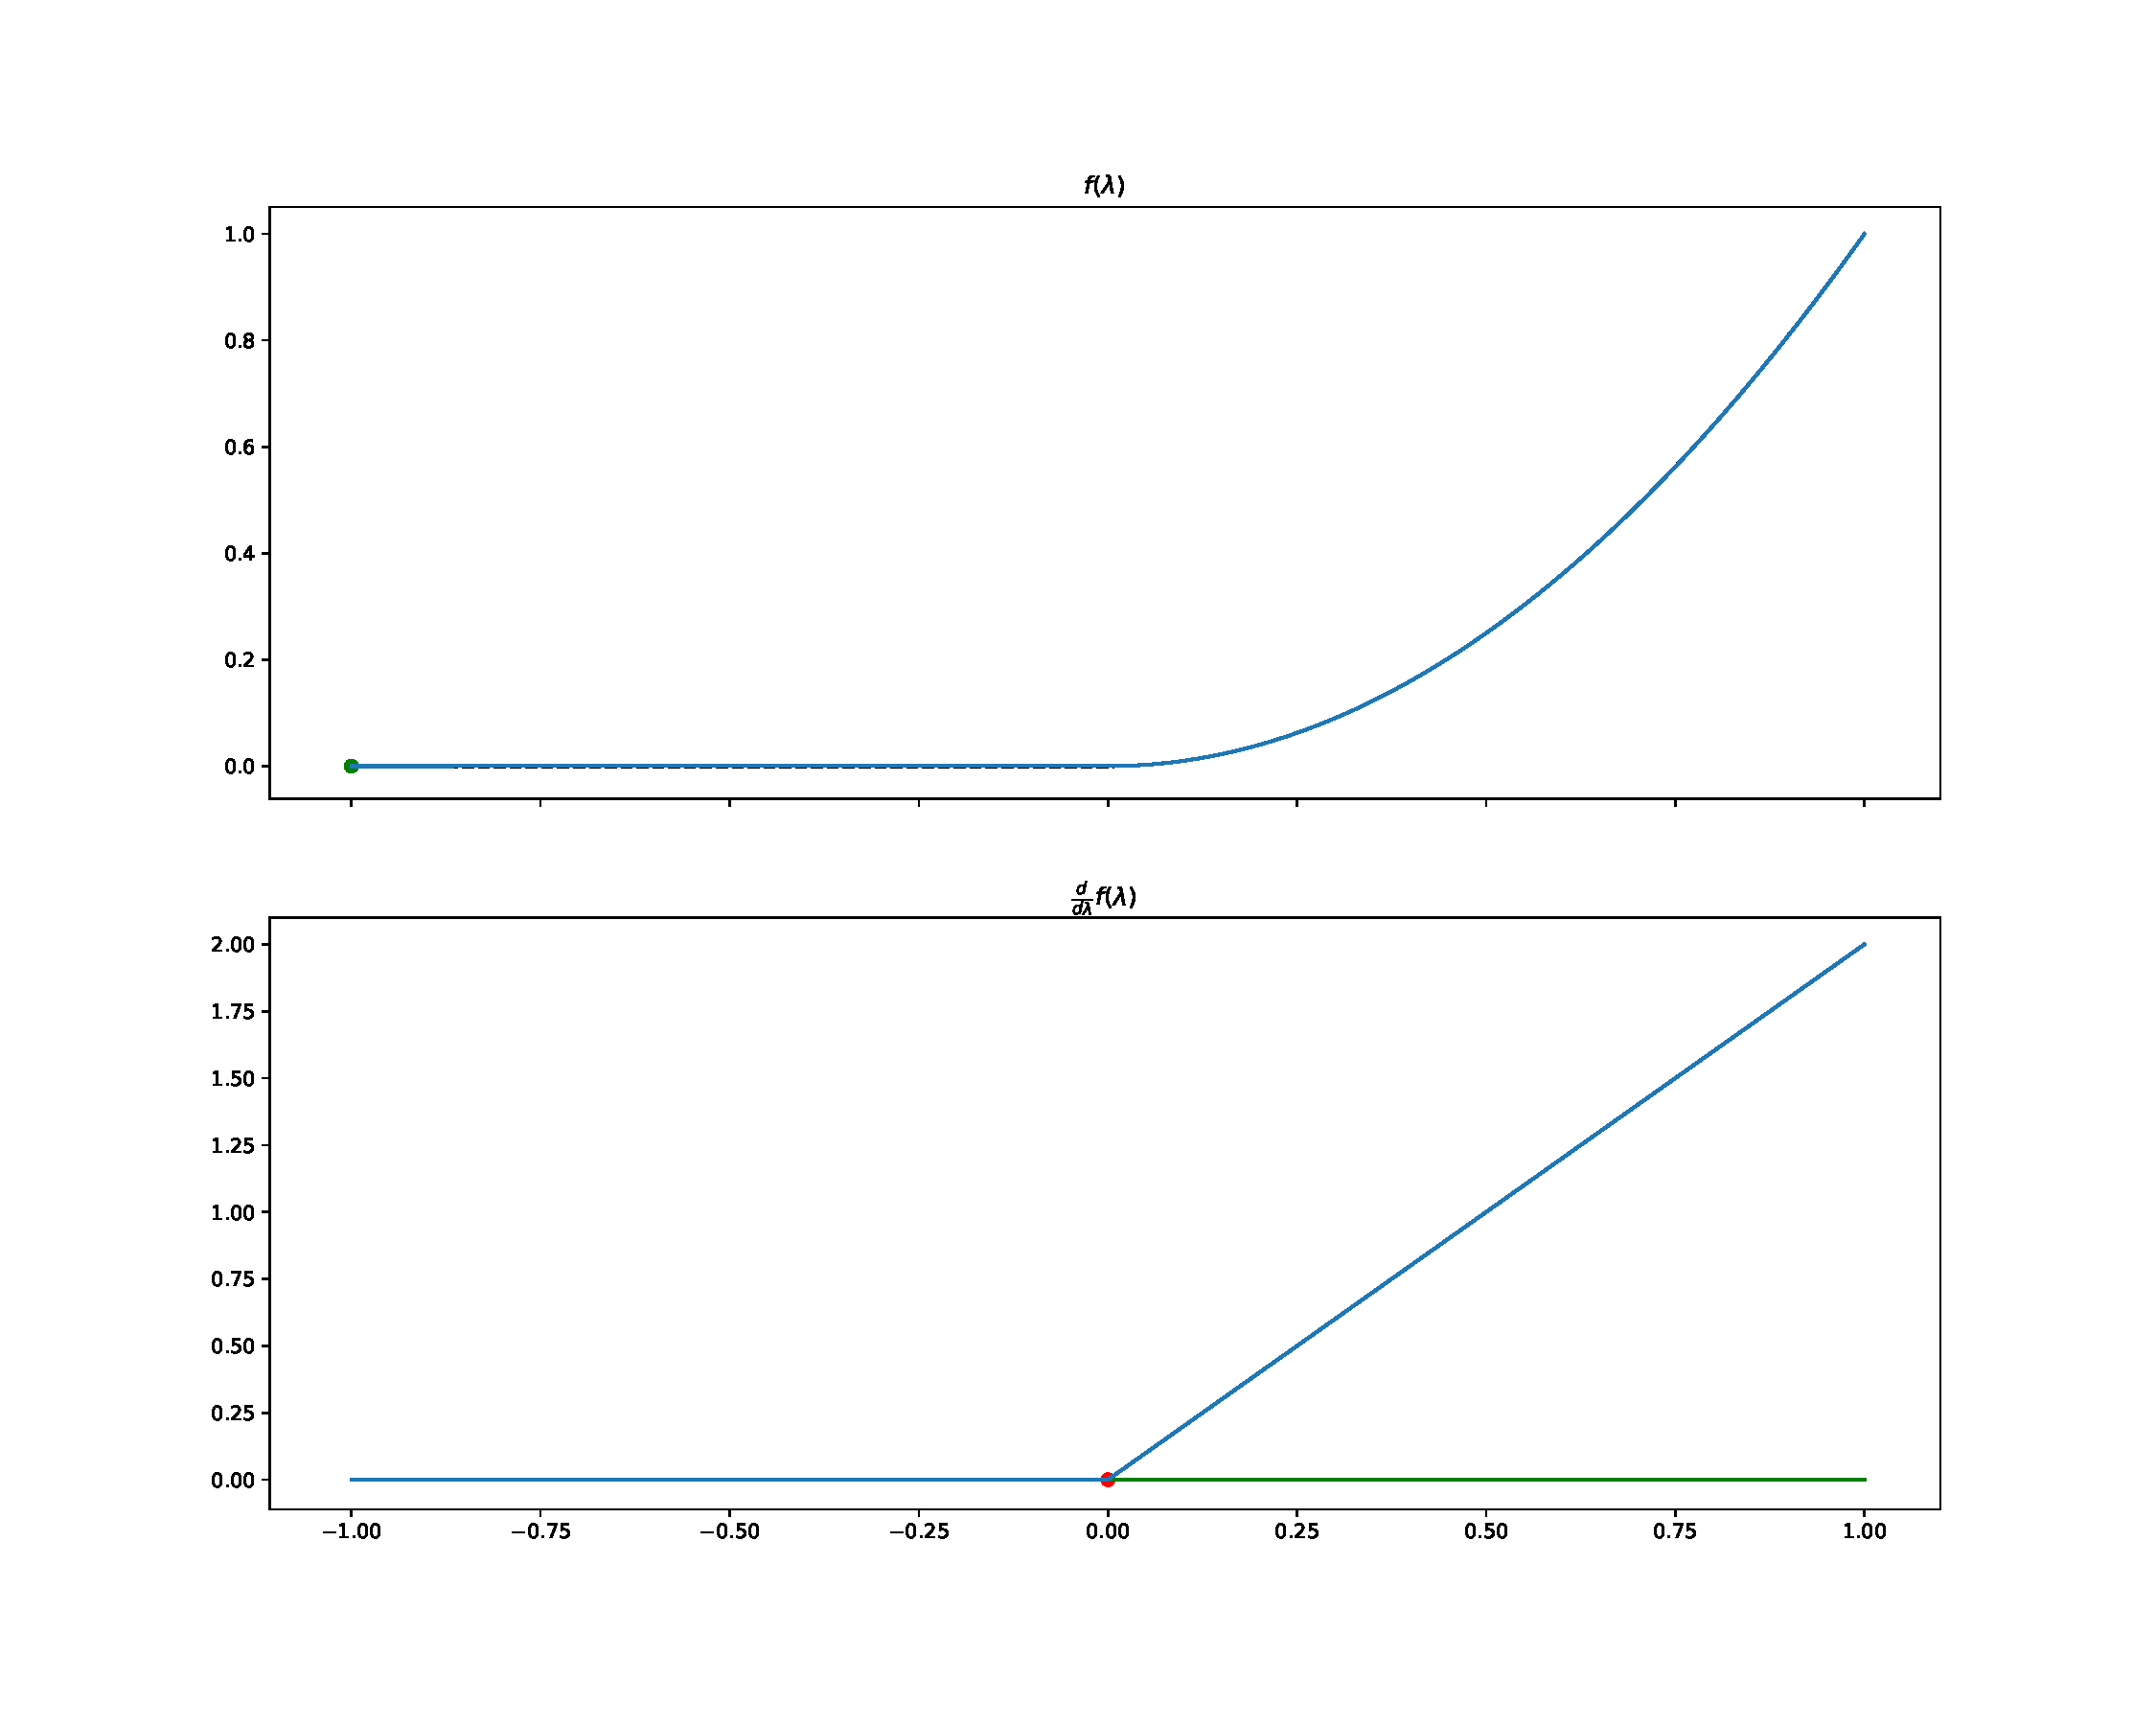
\includegraphics[width=\textwidth]{Chapter4/NeuroCom2021/ejemplo1_sqhinge.pdf}
    \caption{Positive part function (top) and its corresponding subgradient (bottom). The green line represents the $0$ constant function. The yellow dot indicates one point minimizing the function.}
    \label{fig:sqhinge_loss}
\end{figure}
Using the formulation of~\eqref{eq:subproblem_lambda}, the training error corresponding to the hinge loss is
\begin{equation}
    \label{eq:opt_hinge_l2}
    \argmin_{\lambda \in [0, 1]} \mathcal{J}(\lambda) = \sum_{i=1}^{\npertask} \pospart{\lambda c_i + d_i}^2.
\end{equation}
In each term of the sum the subdifferential is 
\begin{equation}
    \label{eq:subdiff_hinge_l2}
    \begin{aligned}
        \partial \left[\lambda c_i + d_i \right]_+^2 = 
    \begin{cases}
        0 &, \lambda c_i + d_i  \leq 0 \\
        2 c_i (\lambda c_i + d_i) &, \lambda c_i + d_i  > 0 \\
    \end{cases} \; .
    \end{aligned}
\end{equation}
The elbows are again related to the values $\frac{-d_i}{c_i}$, that can be sorted to obtain the elbows ${\lambda}_{(1)} < \ldots < {\lambda}_{(m)}$.
In~\citet[Proposition 2]{RuizAD21} we give the following result to get the optimal $\lambda^*$ when using the squared hinge loss.
\begin{prop}[Optimal $\lambda^*$ with squared hinge loss]\label{prop:sqhinge_neurocom2020}
    In~\eqref{eq:opt_hinge_l2},
    $\lambda^*=0$ is optimal iff 
    \begin{equation}\nonumber
        -\sum_{\substack{i:\; 0 > c_{(i)},\\ \;\; 0 < \lambda_{(i)}}} {2 c_i d_i} - \sum_{\substack{i:\; 0 < c_{(i)},\\ \;\; 0 > \lambda_{(i)}}} {2 c_i d_i}  \leq 0
       \end{equation}
    If this condition does not hold, 
    consider the extended sorted list of elbows $\lambda_{(1)}, \ldots, \lambda_{(\npertask)}$, then we define $\widehat{\lambda}_k$ for $k=1, \ldots,  \npertask-1$ as %
\begin{equation}\label{eq:sol_hinge_2}
    \widehat{\lambda}_{(k)} = - \frac{\sum_{i:\; \lambda_{(k+1)} \geq \lambda_{(i)}} \mymax{0, c_{(i)}} d_{(i)} + \sum_{i:\; \lambda_{(k)} \leq \lambda_{(i)}} \mymin{0, c_{(i)}} d_{(i)}}{\sum_{i:\; \lambda_{(k+1)} \geq \lambda_{(i)}} \mymax{0, c_{(i)}}^2 + \sum_{i:\; \lambda_{(k)} \leq \lambda_{(i)}} \mymin{0, c_{(i)}}^2} .
\end{equation}
%
If $\lambda_{(k)} \leq \widehat{\lambda}_k \leq  \lambda_{(k+1)}$ and $0 \leq \widehat{\lambda}_{(k)} \leq 1$ for some $k=1, \ldots, \npertask$, then $\lambda^* = \widehat{\lambda}_k$ is optimal.
Finally, if none of the previous conditions holds, \eqref{eq:opt_hinge_l2} has a minimum at $\lambda^* = 1$.
\end{prop}
\begin{proof}
    Observe in~\eqref{eq:subdiff_hinge_l2} that, for each term $\partial \abs{\lambda c_i + d_i}$, the change occurs at the elbow $\lambda_{i} = - d_ i / c_i$. We can consider two cases:
    \begin{itemize}
        \item $0 > c_i$, then
        \begin{equation}
            \nonumber
            \begin{aligned}
                \partial \pospart{\lambda c_i + d_i}^2 = 
                \begin{cases}
                    0 &, \lambda \geq \lambda_i \\
                    2 c_i (\lambda c_i + d_i) &, \lambda < \lambda_i \\
                \end{cases}
            \end{aligned}
        \end{equation}
        \item $0 < c_i$, then
        \begin{equation}
            \nonumber
            \begin{aligned}
                \partial \pospart{\lambda c_i + d_i}^2 = 
                \begin{cases}
                    0 &, \lambda \leq \lambda_i \\
                    2 c_i (\lambda c_i + d_i) &, \lambda > \lambda_i \\
                \end{cases}
            \end{aligned}
        \end{equation}
    \end{itemize}
    Consider the sorted elbow values $\lambda_{(1)}, \ldots, \lambda_{(m)}$.
    Recall that, since all functions share the same domain, the gradient of the sum is the gradient sum of the gradients, then, for all $\lambda \in \reals$,
    \begin{equation}\nonumber
        \begin{aligned}
            \partial \mathcal{J}(\lambda) &=  \sum_{\substack{i:\; 0 > c_{(i)},\\ \;\; \lambda < \lambda_{(i)}}} {2 c_i (\lambda c_i + d_i)} + \sum_{\substack{i:\; 0 < c_{(i)},\\ \;\; \lambda > \lambda_{(i)}}} {2 c_i (\lambda c_i + d_i)}  .
        \end{aligned}        
    \end{equation}
    Observe that in both terms of the sum, $(\lambda c_i + d_i) > 0$, so the first term is negative and the second one positive; then, $\partial \mathcal{J}(\lambda)$ is a non-decreasing function.
    Also, we can check that $\partial \mathcal{J}(\lambda)$ is continuous. It is trivially continuous between elbows, and, at any elbow $\lambda_{(k)}$, 
    $$
    \partial \mathcal{J}(\lambda_{(k)}) =  \sum_{\substack{i:\; 0 > c_{(i)},\\ \;\; \lambda_{(k)} < \lambda_{(i)}}} {2 c_i (\lambda_{(k)} c_i + d_i)} + \sum_{\substack{i:\; 0 < c_{(i)},\\ \;\; \lambda_{(k)} > \lambda_{(i)}}} {2 c_i (\lambda_{(k)} c_i + d_i)}  ,
    $$
    and also, the left limit is 
    \begin{align*}
        \lim_{\lambda \to \lambda_{(k)}^{-}} \partial \mathcal{J}(\lambda_{(k)}) &= 
        2c_{(k)} (\lambda c_{(k)} + d_{(k)})  + 
        \sum_{\substack{i:\; 0 > c_{(i)},\\ \;\; \lambda_{(k)} < \lambda_{(i)}}} {2 c_i (\lambda c_i + d_i)} + \sum_{\substack{i:\; 0 < c_{(i)} ,\\ \;\; \lambda_{(k)} > \lambda_{(i)}}} {2 c_i (\lambda c_i + d_i)},
    \end{align*}
    and the first term goes to zero, so the limit is $\partial \mathcal{J}(\lambda_{(k)})$. Analogously, we can find that the right limit is also $\partial \mathcal{J}(\lambda_{(k)})$.    
    That is, $\partial \mathcal{J}(\lambda)$ is piece-wise defined, but it is continuous and non-decreasing; thus, using the Fermat rule, we want to find $\lambda^*$ such that $\partial \mathcal{J}(\lambda^*) = 0$. We have three possible scenarios:
    \begin{itemize}
        \item $\partial \mathcal{J}(0) \geq 0.$ 
        \\Since $\partial \mathcal{J}(\lambda)$ is non-decreasing, the optimal value in $[0, 1]$ is $\lambda^* = 0$.
        \item $0 = \partial \mathcal{J}(\lambda), \; 0 < \lambda < 1$. 
        \\ Between each pair of elbows $(\lambda_{(k)}, \lambda_{(k+1)})$, for $k=1,  \dots, \npertask-1$, 
        \begin{equation}\nonumber
            \begin{aligned}
                \partial \mathcal{J}(\lambda) &=  \sum_{\substack{i:\; 0 > c_{(i)},\\ \;\; \lambda_{(k)} \leq \lambda_{(i)}}} {2 c_i (\lambda c_i + d_i)} + \sum_{\substack{i:\; 0 < c_{(i)},\\ \;\; \lambda_{(k+1)} \geq \lambda_{(i)}}} {2 c_i (\lambda c_i + d_i)}  ;
            \end{aligned}        
        \end{equation}
        then, $\partial \mathcal{J}(\lambda) = 0$ has the solution
        \begin{equation}
            \nonumber
            \widehat{\lambda}_{(k)} = - \frac{\sum_{i:\; \lambda_{(k+1)} \geq \lambda_{(i)}} \mymax{0, c_{(i)}} d_{(i)} + \sum_{i:\; \lambda_{(k)} \leq \lambda_{(i)}} \mymin{0, c_{(i)}} d_{(i)}}{\sum_{i:\; \lambda_{(k+1)} \geq \lambda_{(i)}} \mymax{0, c_{(i)}}^2 + \sum_{i:\; \lambda_{(k)} \leq \lambda_{(i)}} \mymin{0, c_{(i)}}^2} .
        \end{equation}
        If $\lambda_{(k)} \leq \widehat{\lambda}_{(k)} \leq \lambda_{(k+1)}$ and $0 \leq \widehat{\lambda}_{(k)} \leq 1$, the optimal value is $\lambda^* = \widehat{\lambda}_{(k)}$.
        \item $\partial \mathcal{J}(1) \leq 0$. 
        \\None of the previous conditions hold, and since $\partial \mathcal{J}(\lambda)$ is non-decreasing, the optimal value in $[0, 1]$ is $\lambda^* = 1$.
    \end{itemize}
\end{proof}


\begin{figure}[t!]
    \centering
    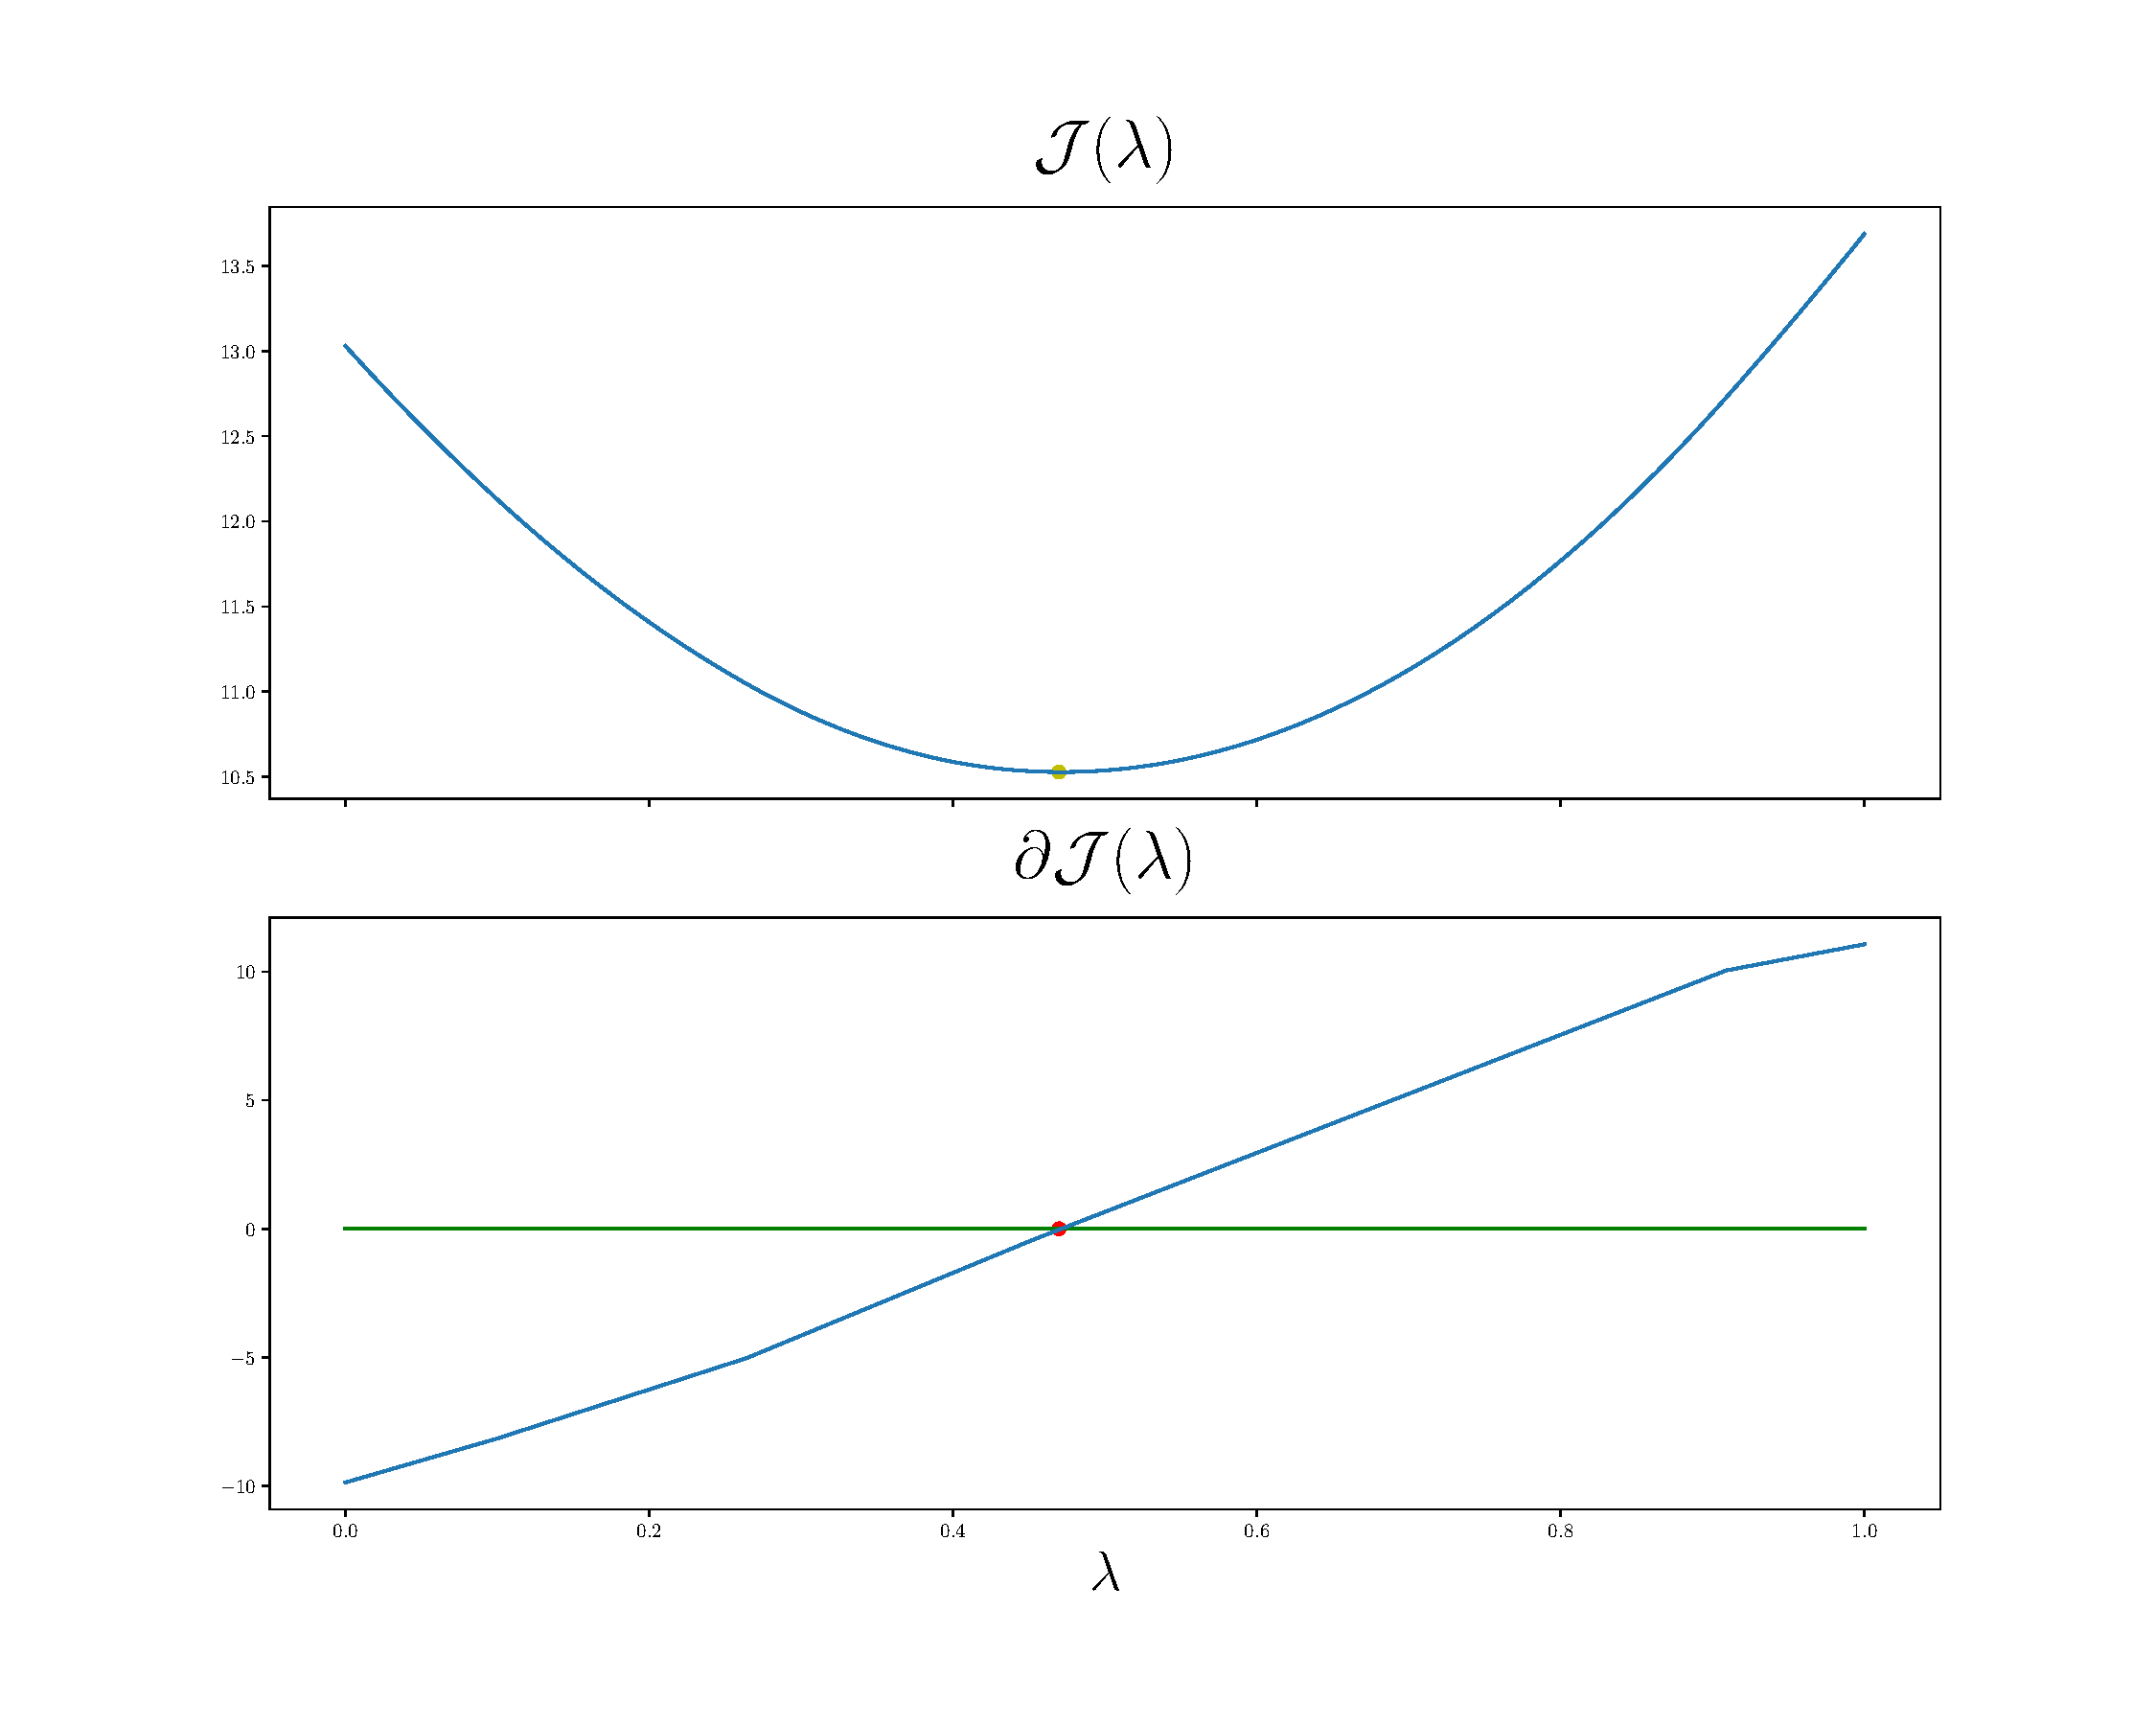
\includegraphics[width=\textwidth]{Chapter4/NeuroCom2021/ejemplo2_sqhinge.pdf}
    \caption{Error using the squared hinge loss function (top) and its corresponding subgradient (bottom). The green line represents the $0$ constant function. The yellow dot is the point minimizing the error, whose corresponding derivative is $0$.}
    \label{fig:sqhinge_error}
\end{figure}

As with the other losses, the error function and respective gradient for $10$ random pairs $(c_i, d_i)$ are represented in Figure~\ref{fig:sqhinge_error}.
Now, the derivative is not constant between elbows, but a linear function, and we can observe that the derivative is continuous. 

As with the two previous losses, once the elbows are sorted, the numerator and denominator that appear in~\eqref{eq:sol_hinge_2} can be computed with a linear cost. For example, consider the sequence of numerators $N_{(k)} = \sum_{i:\; \lambda_{(k+1)} \geq \lambda_{(i)}} \mymax{0, c_{(i)}} d_{(i)} + \sum_{i:\; \lambda_{(k)} \leq \lambda_{(i)}} \mymin{0, c_{(i)}} d_{(i)}$; then, 
$$N_{(k+1)} = N_{(k)} - \mymax{0, c_{(k+1)}} d_{(k+1)} + \mymin{0, c_{(k+1)}} d_{(k+1)}.$$
Analogously, for the sequence of denominators $D_{(k)} = \sum_{i:\; \lambda_{(k+1)} \geq \lambda_{(i)}} \mymax{0, c_{(i)}} d_{(i)} + \sum_{i:\; \lambda_{(k)} \leq \lambda_{(i)}} \mymin{0, c_{(i)}} d_{(i)}$, we have that 
$$D_{(k+1)} = D_{(k)} - \mymax{0, c_{(k+1)}}^2 + \mymin{0, c_{(k+1)}}^2.$$
Then, at each step $k=1, \ldots, \npertask-1$ we compute $\widehat{\lambda}_{(k)}$ and check if $\lambda_{(k)} \leq \widehat{\lambda}_{(k)} \leq \lambda_{(k+1)}$ and $0 \leq \widehat{\lambda}_{(k)} \leq 1$.
Therefore, again we have that the largest cost is the one corresponding to sorting the elbows, which is in average $O(\npertask \log(\npertask))$.

%Between elbows $\lambda_{(k)}$ and $\lambda_{(k+1)}$ the derivative is
%$$ \lambda \left(\sum_{j:\; \lambda_{(j)} < \lambda_{(k)}} \max(0, c_{j})^2 + \sum_{j:\; \lambda_{(j)} > \lambda_{(k)}} \min(0, c_{j})^2 \right) + \sum_{j:\; \lambda_{j} < 0} \max(0, c_{j}) d_{j} + \sum_{j:\; \lambda_{j} > 0} \min(0, c_{j}) d_{j}, $$
%and it is $0$ for the value $\widehat{\lambda}_k$ shown in~\eqref{eq:opt_hinge_l2}; however, that value is optimal only if $\lambda_{(k)} \leq \widehat{\lambda}_k \leq  \lambda_{(k+1)}$.



\section{Conclusions}\label{sec-conclusions-3}

In this chapter, we have\dots
